\PassOptionsToPackage{unicode=true}{hyperref} % options for packages loaded elsewhere
\PassOptionsToPackage{hyphens}{url}
%
\documentclass[]{article}
\usepackage{lmodern}
\usepackage{amssymb,amsmath}
\usepackage{ifxetex,ifluatex}
\usepackage{fixltx2e} % provides \textsubscript
\ifnum 0\ifxetex 1\fi\ifluatex 1\fi=0 % if pdftex
  \usepackage[T1]{fontenc}
  \usepackage[utf8]{inputenc}
  \usepackage{textcomp} % provides euro and other symbols
\else % if luatex or xelatex
  \usepackage{unicode-math}
  \defaultfontfeatures{Ligatures=TeX,Scale=MatchLowercase}
\fi
% use upquote if available, for straight quotes in verbatim environments
\IfFileExists{upquote.sty}{\usepackage{upquote}}{}
% use microtype if available
\IfFileExists{microtype.sty}{%
\usepackage[]{microtype}
\UseMicrotypeSet[protrusion]{basicmath} % disable protrusion for tt fonts
}{}
\IfFileExists{parskip.sty}{%
\usepackage{parskip}
}{% else
\setlength{\parindent}{0pt}
\setlength{\parskip}{6pt plus 2pt minus 1pt}
}
\usepackage{hyperref}
\hypersetup{
            pdftitle={Appendix: SEPSIS Trial},
            pdfborder={0 0 0},
            breaklinks=true}
\urlstyle{same}  % don't use monospace font for urls
\usepackage[margin=1in]{geometry}
\usepackage{graphicx,grffile}
\makeatletter
\def\maxwidth{\ifdim\Gin@nat@width>\linewidth\linewidth\else\Gin@nat@width\fi}
\def\maxheight{\ifdim\Gin@nat@height>\textheight\textheight\else\Gin@nat@height\fi}
\makeatother
% Scale images if necessary, so that they will not overflow the page
% margins by default, and it is still possible to overwrite the defaults
% using explicit options in \includegraphics[width, height, ...]{}
\setkeys{Gin}{width=\maxwidth,height=\maxheight,keepaspectratio}
\setlength{\emergencystretch}{3em}  % prevent overfull lines
\providecommand{\tightlist}{%
  \setlength{\itemsep}{0pt}\setlength{\parskip}{0pt}}
\setcounter{secnumdepth}{0}
% Redefines (sub)paragraphs to behave more like sections
\ifx\paragraph\undefined\else
\let\oldparagraph\paragraph
\renewcommand{\paragraph}[1]{\oldparagraph{#1}\mbox{}}
\fi
\ifx\subparagraph\undefined\else
\let\oldsubparagraph\subparagraph
\renewcommand{\subparagraph}[1]{\oldsubparagraph{#1}\mbox{}}
\fi

% set default figure placement to htbp
\makeatletter
\def\fps@figure{htbp}
\makeatother

\renewcommand{\topfraction}{.85}
\renewcommand{\bottomfraction}{.7}
\renewcommand{\textfraction}{.15}
\renewcommand{\floatpagefraction}{.66}
\setcounter{topnumber}{3}
\setcounter{bottomnumber}{3}
\setcounter{totalnumber}{4}
\usepackage{caption}
\usepackage{float}
\usepackage{subcaption}
\floatplacement{figure}{H}

\title{Appendix: SEPSIS Trial}
\author{}
\date{\vspace{-2.5em}}

\begin{document}
\maketitle

2020-09-09

\hypertarget{stopping-with-moderately-permissive-outcome-p1}{%
\subsection{Stopping with moderately permissive outcome
(p1)}\label{stopping-with-moderately-permissive-outcome-p1}}

Both superiority and futility decisions were made with respect to the
moderately permissive outcome (p1). Unless stated otherwise, the
futility bound used was 0.4 and a probability threshold of 0.975 was
required to stop for futility.

\hypertarget{type-i-error-false-positive-risk}{%
\subparagraph{Type I error (false positive
risk)}\label{type-i-error-false-positive-risk}}

Figure 1 displays the overall type I error rate for the simulations
where early stopping is based on interim results from the moderately
permissive outcome. The type I error is under good control (i.e.,
\textless{}5\%) for outcomes s and p2 since repeated superiority testing
is only occurring for outcome p1. Specifically, the type I error for the
three superiority thresholds 0.95, 0.975, 0.99 for these outcomes are
approximately 5\%, 2.5\%, and \textless{}1\%. For outcome p1, the type I
error is approximately 15\%, 10\%, and 5\% for the three superiority
thresholds. As such, the 0.95 and 0.975 superiority thresholds do not
appear to retain adequate control of the type I error for p1.

\captionsetup[figure]{font=small,labelfont=small}

\begin{figure}
  \caption{Overall type I error rate based on moderately permissive (p1) outcome based stopping rules. Observed type one
  error rate for each outcome is presented by colored bars (see legend). Results by the three categories of control
  event rates are by rows. Results by the three superiority thresholds are presented by columns. Results by the futility
  thresholds are presented by the x-axis within each sub plot.}
  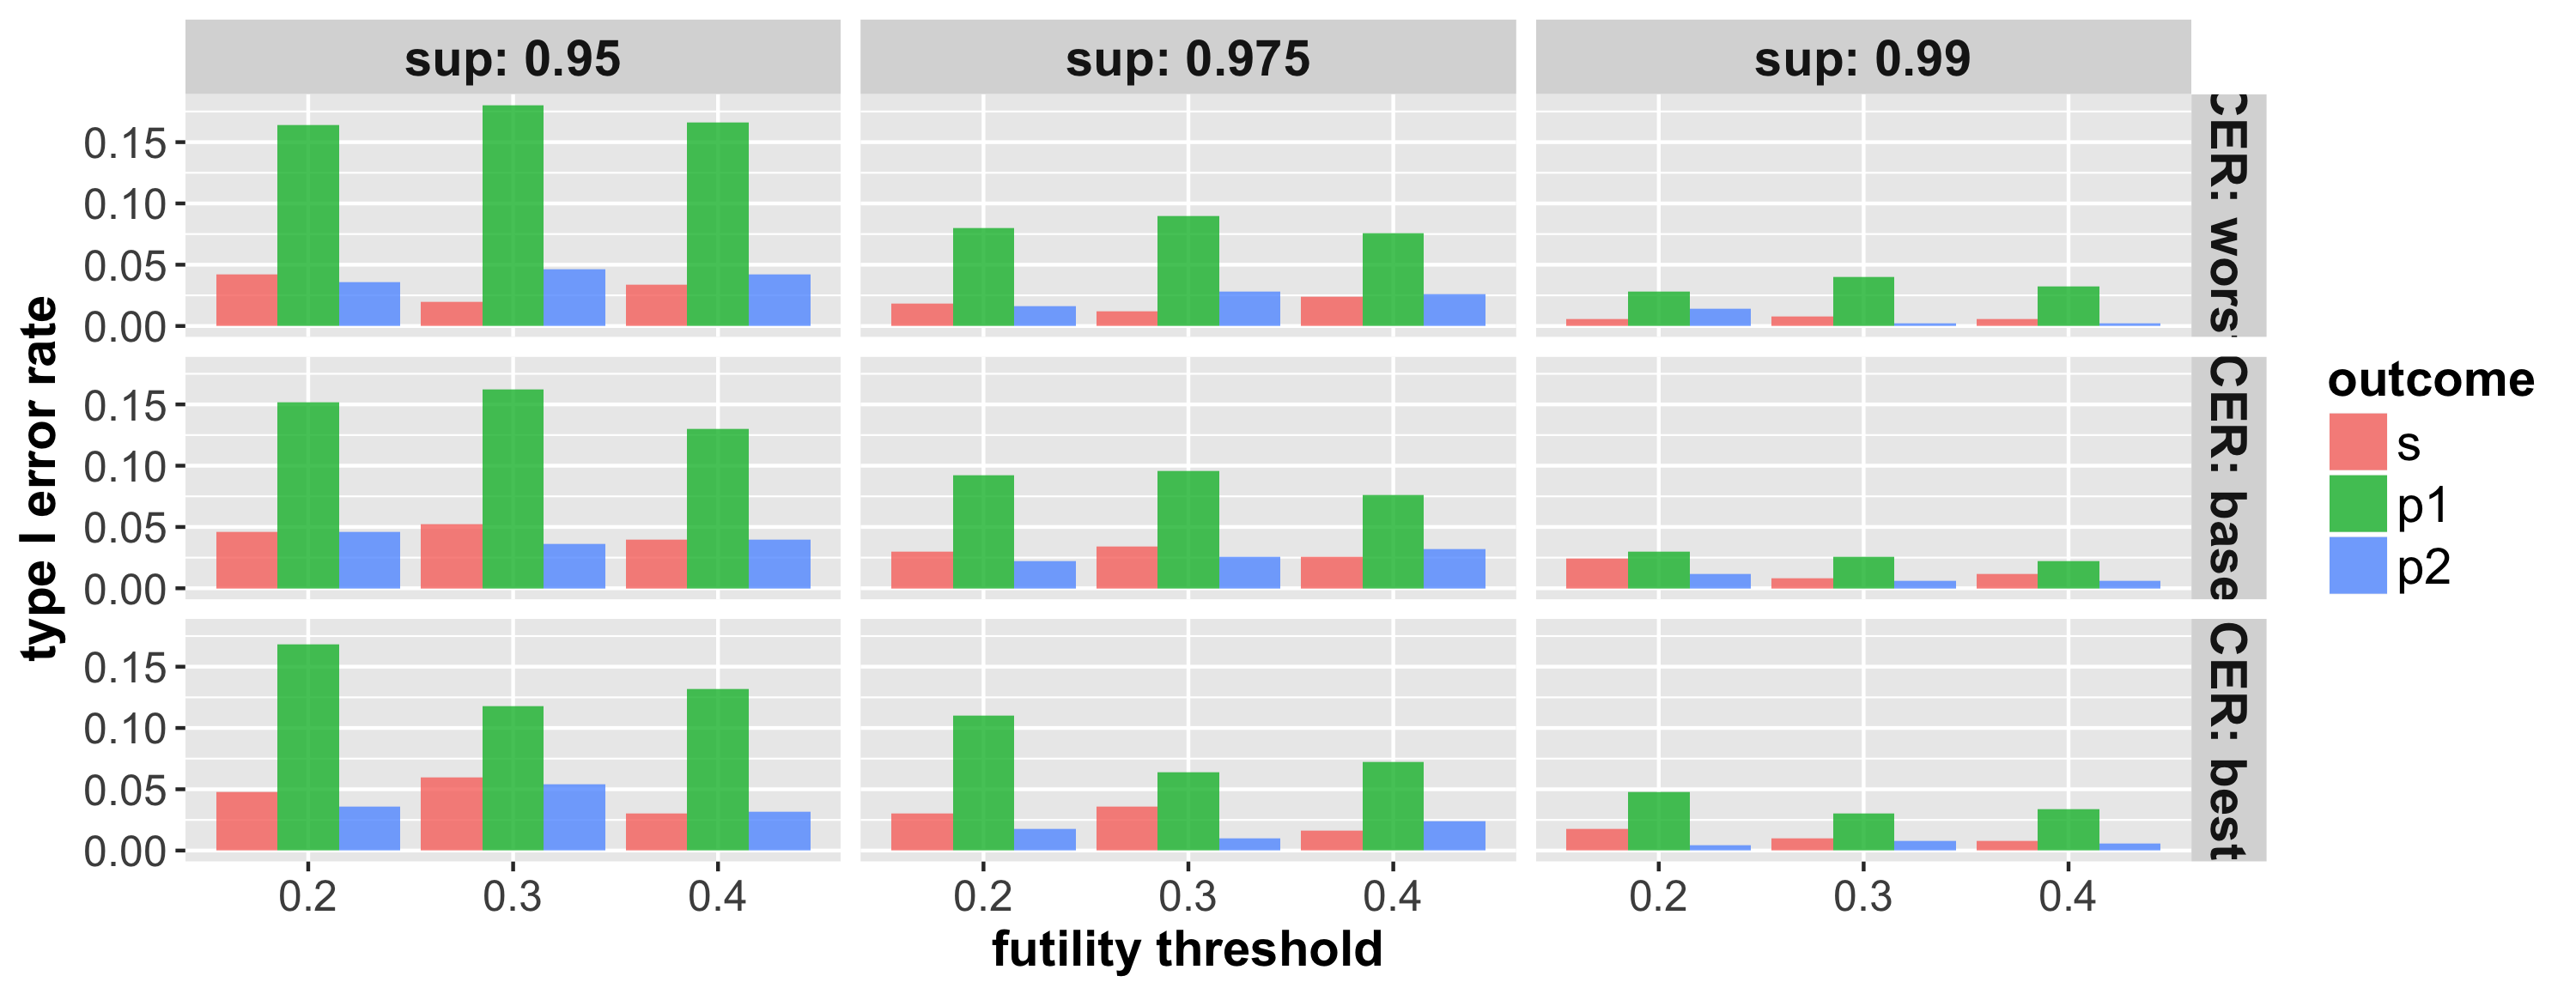
\includegraphics{../plots/stop_p1_new/alpha_sim_05_stopp1_new.png}
\end{figure}

\hypertarget{power}{%
\subparagraph{Power}\label{power}}

Figure 2 displays the power for each of the outcomes under each of the
simulated scenarios and employed stopping rules. Generally, the power to
detect an effect is high for outcome p2 in all scenarios, with only a
moderate reduction in power when the true RRR=20\%. The power to detect
an effect for outcome p1 is high in all scenarios where RRR=40\% or
60\%, but moderate to low when RRR=20\%. For RRR=20\%, the power to
detect p1 generally decreases as the superiority threshold increases and
the CER goes from best to worst. The power to detect an effect on
outcome s is low in all cases, but achieves its highest estimates when
RRR=60\% and CER best case scenario.

\begin{figure}
  \caption{Power under the three relative risk reductions (RRR - upper column label) for each of the outcomes (lower
  column labels). Power estimates by control event rates are presented by the rows. Power estimated for superiority
  thresholds are presented by the sub-plot x-axis. Power estimates by the futility thresholds are presented by the bar
  color (see legend).}
  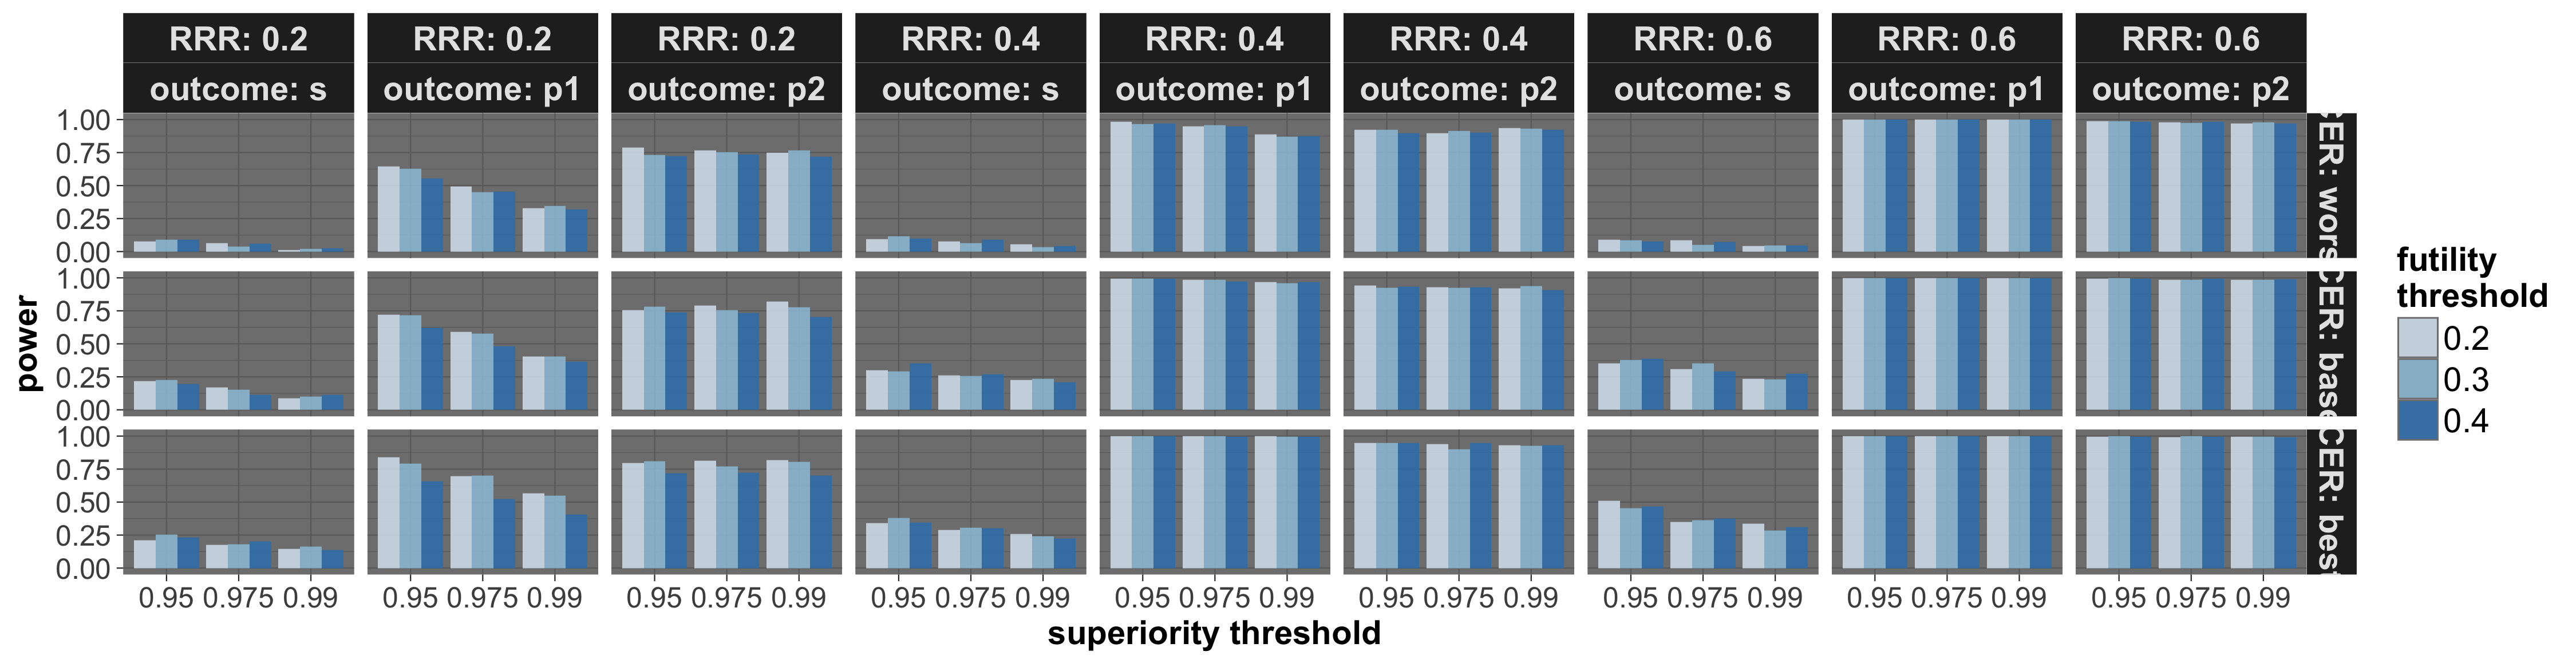
\includegraphics{../plots/stop_p1_new/power_all_sim_05_stopp1_new.png}
\end{figure}

Figure 3. Under the true RRR=40\% and 60\%, power for outcomes p1 and p2
is very high but decreases to roughly 50-75\% for the true RRR=20\%.
Power for outcome s is low for all scenarios, reaching roughly 25\% for
a true RRR=60\% and the best case CER.

\begin{figure}
  \caption{Power under the three relative risk reductions (RRR - upper column label) for each of the outcomes (lower
  column labels or legend). Observed power for each outcome is presented by colored bars. Power estimates by control
  event rates are presented by the rows and correspond to a futility bound of 0.4 and superiority threshold of 0.975.}
  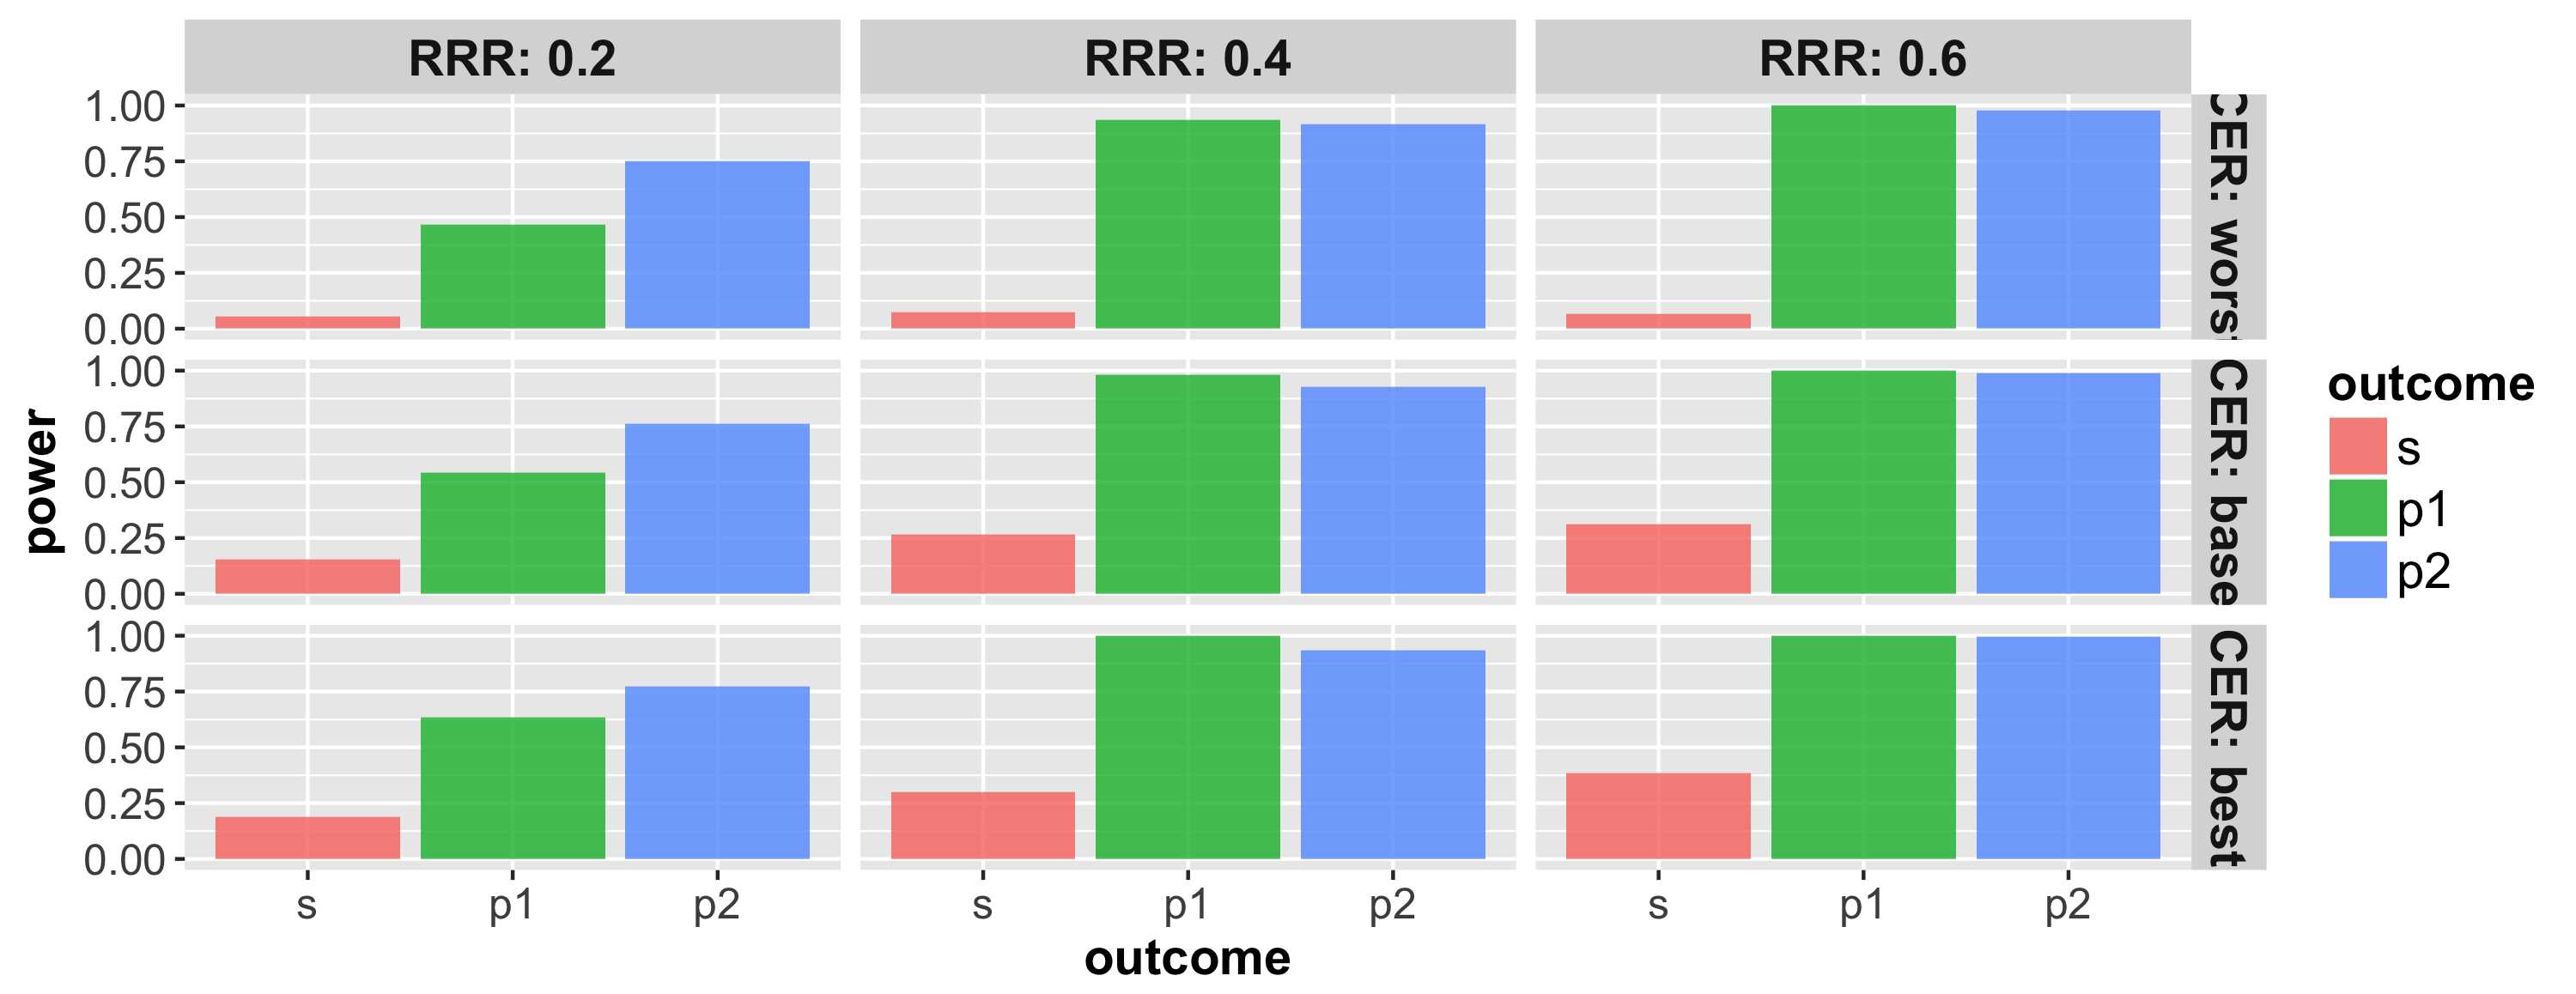
\includegraphics{../plots/stop_p1_new/power_sim_05_stopp1_new.png}
\end{figure}

\hypertarget{expected-sample-size}{%
\subparagraph{Expected Sample Size}\label{expected-sample-size}}

Figure 4 presents the expected (mean) sample size at trial termination.
For true RRR=0 and RRR=20\%, expected sample sizes were consistently
high, albeit with some notable reductions associated with use of a
RRR=40\% futility stopping threshold. For true of RRR=40\% and RRR=60\%,
expected sample sizes were lower and decreased as the CER improved
(worst to best). Within these RRR, greater superiority thresholds only
marginally increased expected sample size, but futility thresholds had
negligible effects within each superiority threshold.

\begin{figure}
  \caption{Expected sample size at trial termination. Results by control event scenarios are presented by rows. Results
  by relative risk reductions are presented by columns. Results by superiority thresholds are presented by the x-axis of
  the sub-plots, and results by futility thresholds are presented by the color of the bars (see legend).}
  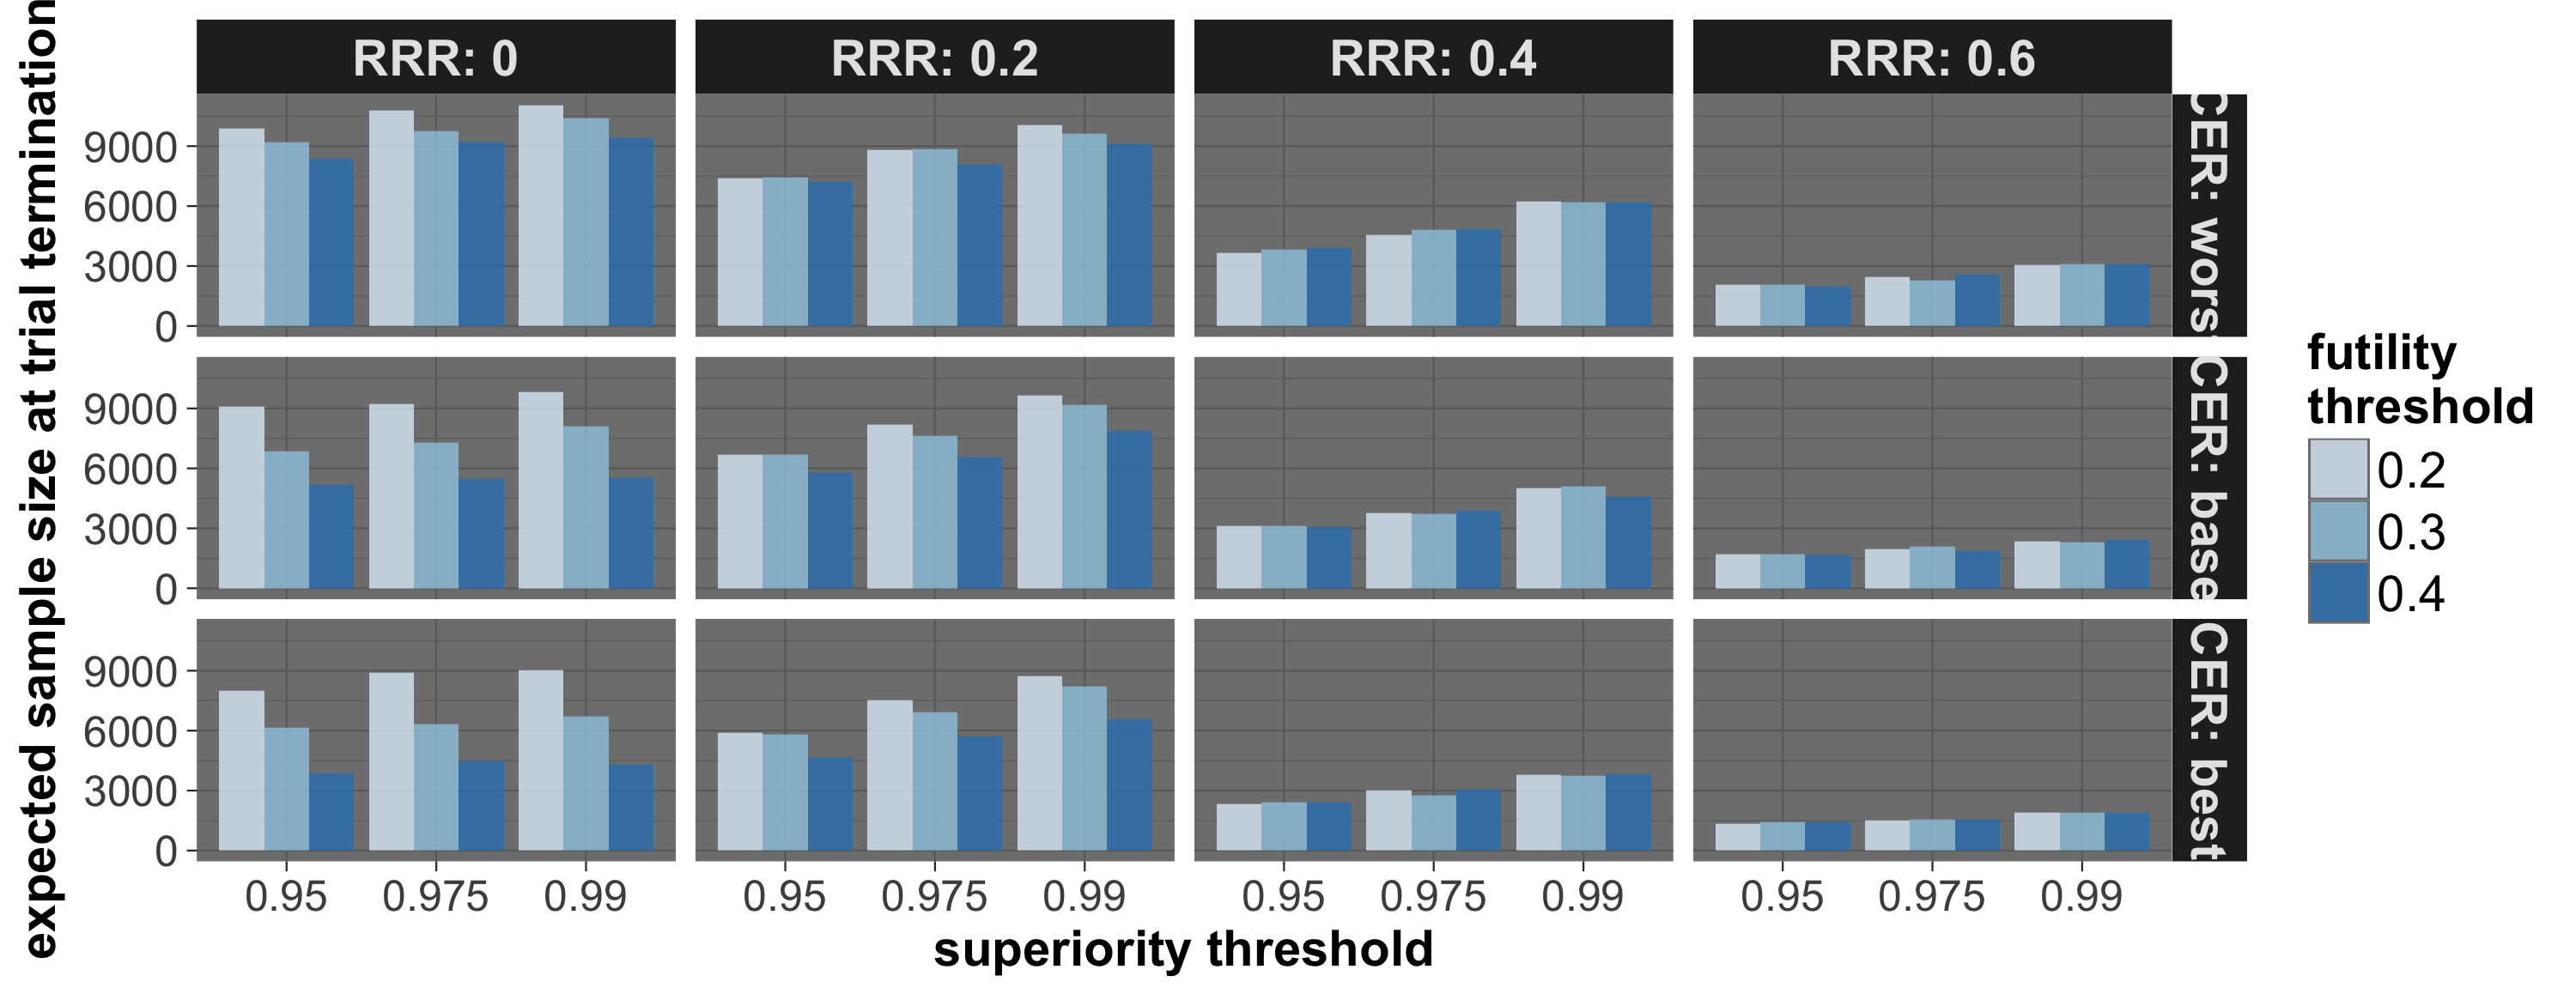
\includegraphics{../plots/stop_p1_new/Nt_sim_05_stopp1_new.png}
\end{figure}

\hypertarget{probability-of-reaching-maximum-sample-size}{%
\paragraph{Probability of Reaching Maximum Sample
Size}\label{probability-of-reaching-maximum-sample-size}}

Figure 5 shows the probability of reaching the maximum allowed sample
size of the trial. This probability was moderate to high for the true
RRR=0 and RRR=20\%, and generally decreased as the CER improved. For
RRR=40\% and RRR=60\%, this probability was negligible for all cases
except RRR=40\% and the worst case CER scenario, where it was roughly
10\% for the highest superiority threshold.

\begin{figure}
  \caption{Probability of reaching maximum sample size for the three control event rates (CER – rows), four relative
  risk reductions (RRR – columns), three superiority thresholds (x axis) and three futility thresholds (legend).}
  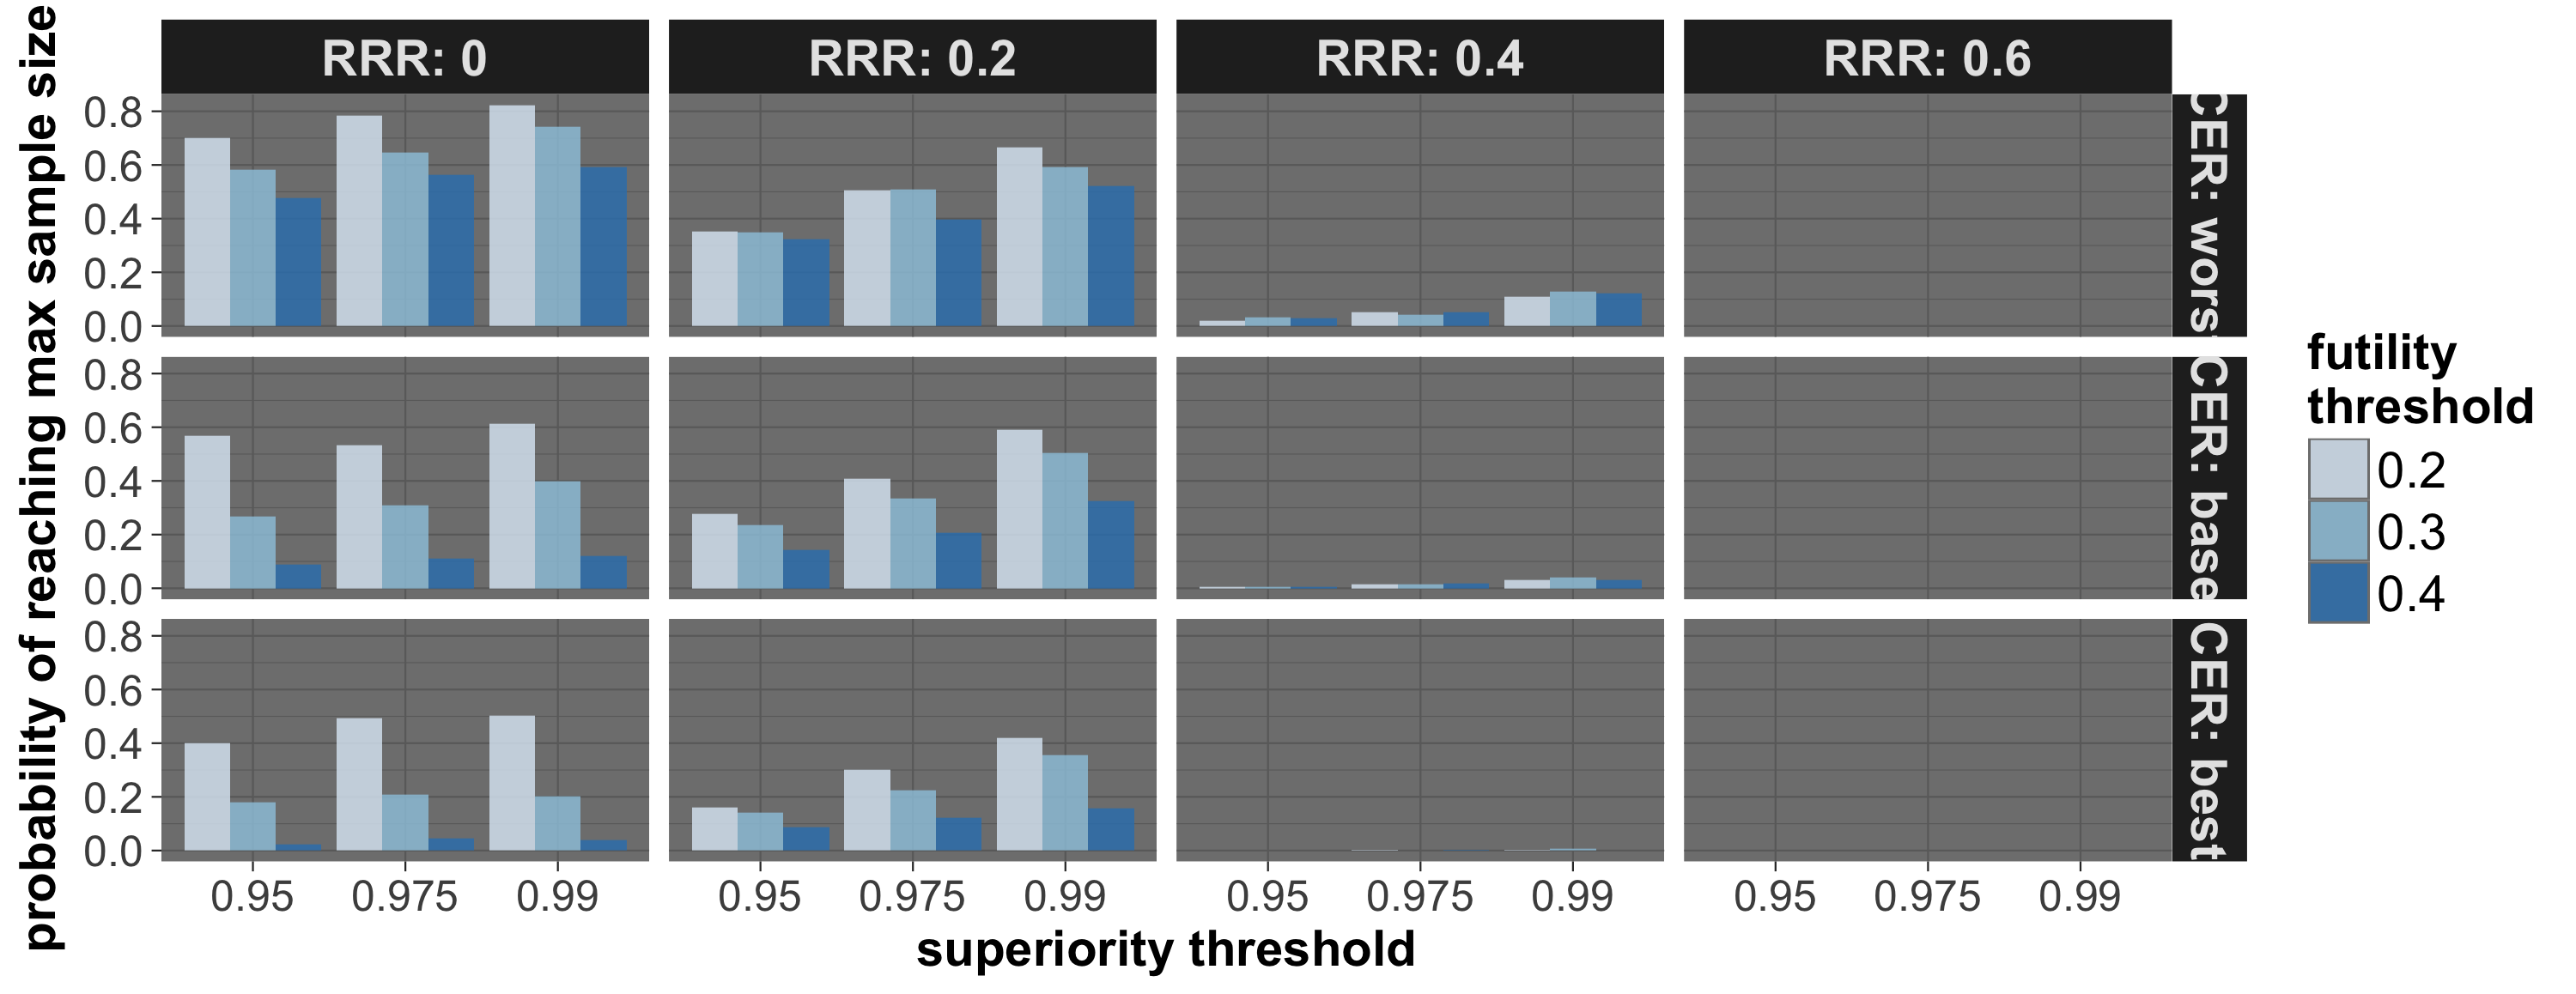
\includegraphics{../plots/stop_p1_new/reachmax_sim_05_stopp1_new.png}
\end{figure}

\hypertarget{probability-of-stopping-early}{%
\paragraph{Probability of Stopping
Early}\label{probability-of-stopping-early}}

The probability of stopping early was obtained overall, for superiority
and for futility. Figure 6 displays the overall probability of stopping
early, Figure 7(a) displays the probability of stopping early for
futility and figure 7(b) displays the probability of stopping early for
superiority. The overall probability of stopping early is strongly
positively correlated with the CER and RRR. When the simulated RRR=0\%
and 20\%, the overall probability of stopping early is also highly
correlated to the futility threshold.

\begin{figure}
  \caption{Probability of stopping early due to futility or superiority for the three control event rates (CER – rows),
  four relative risk reductions (RRR – columns), three superiority thresholds (x axis) and three futility thresholds
  (legend).}
  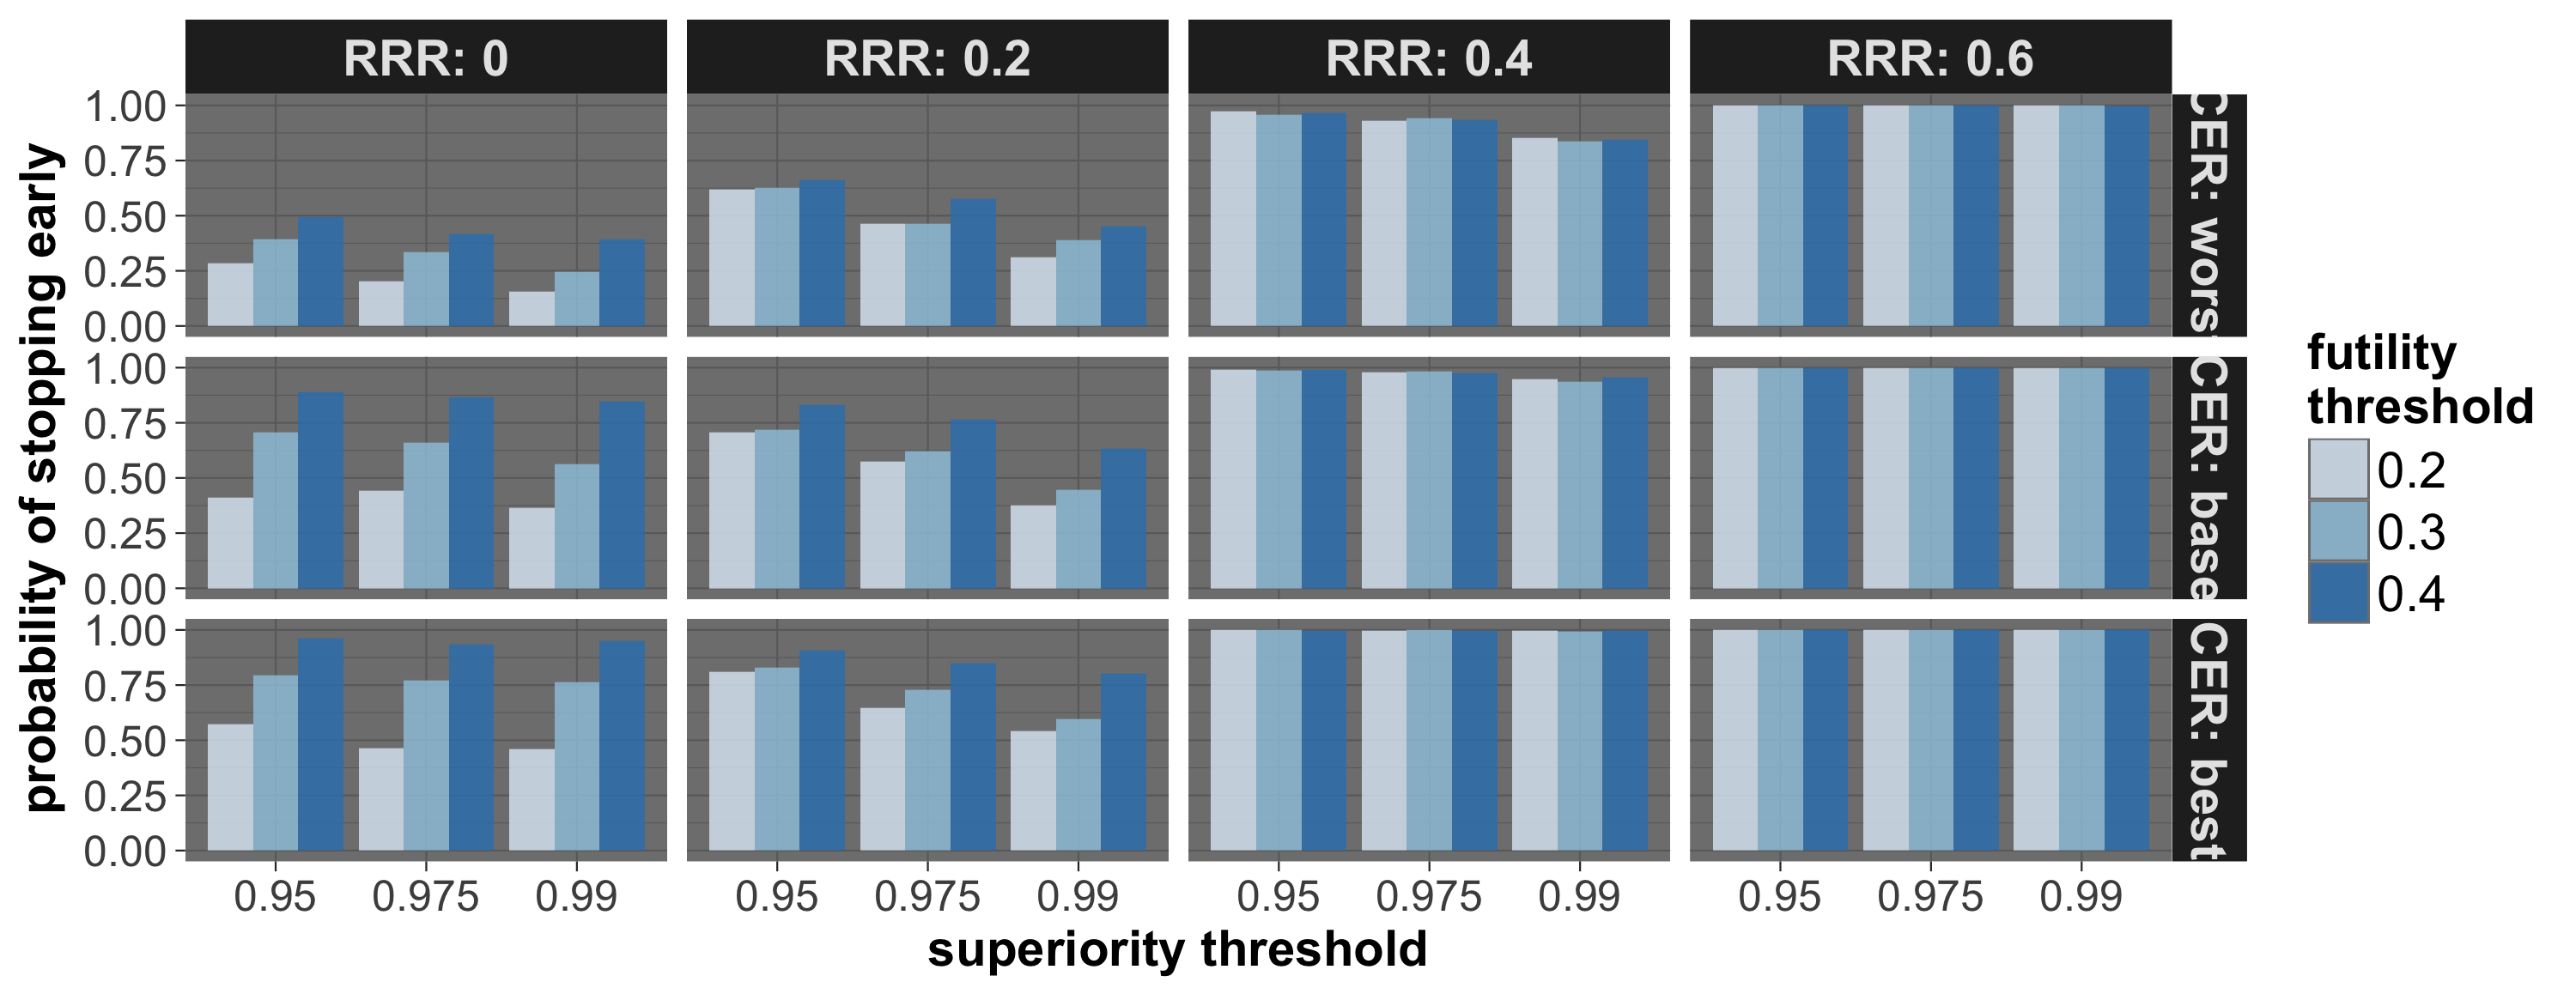
\includegraphics{../plots/stop_p1_new/early_sim_05_stopp1_new.png}
\end{figure}

The RRR=40\% futility threshold results in consistently greater than
80-90\% probability of stopping early for the base and best-case CER
scenarios when true RRR=0\% (similar trend observed for expected sample
size results Figure 3). Stopping early for futility when the simulated
RRR=0\% is likely with futility thresholds of 30\% and 40\%, but less so
with a futility threshold of 20\%. A futility threshold of 40\% also
results in a moderately low probability of stopping early where the true
RRR=20\%. The probability of stopping early for superiority is close to
100\% for all CERs when the true RRR=40\% or RRR=60\%, regardless of
futility threshold. For the true RRR=20\%, there is moderate probability
of stopping early which increases with improving CER and decreases with
higher futility thresholds. The lower probability of stopping for
superiority when the true RRR=0 explained by the high probability of
stopping for futility in this setting.

\begin{figure}
\centering
  \caption{Probability of stopping early due to futility, and stopping early due to superiority. Stopping probabilities
  are presented for the three control event rates (CER – rows), four relative risk reductions (RRR – columns), three
  superiority thresholds (x axis) and three futility thresholds (legend).}
  \label{fig:fig}
  \begin{subfigure}{0.8\textwidth}
    \centering
    \caption{}
    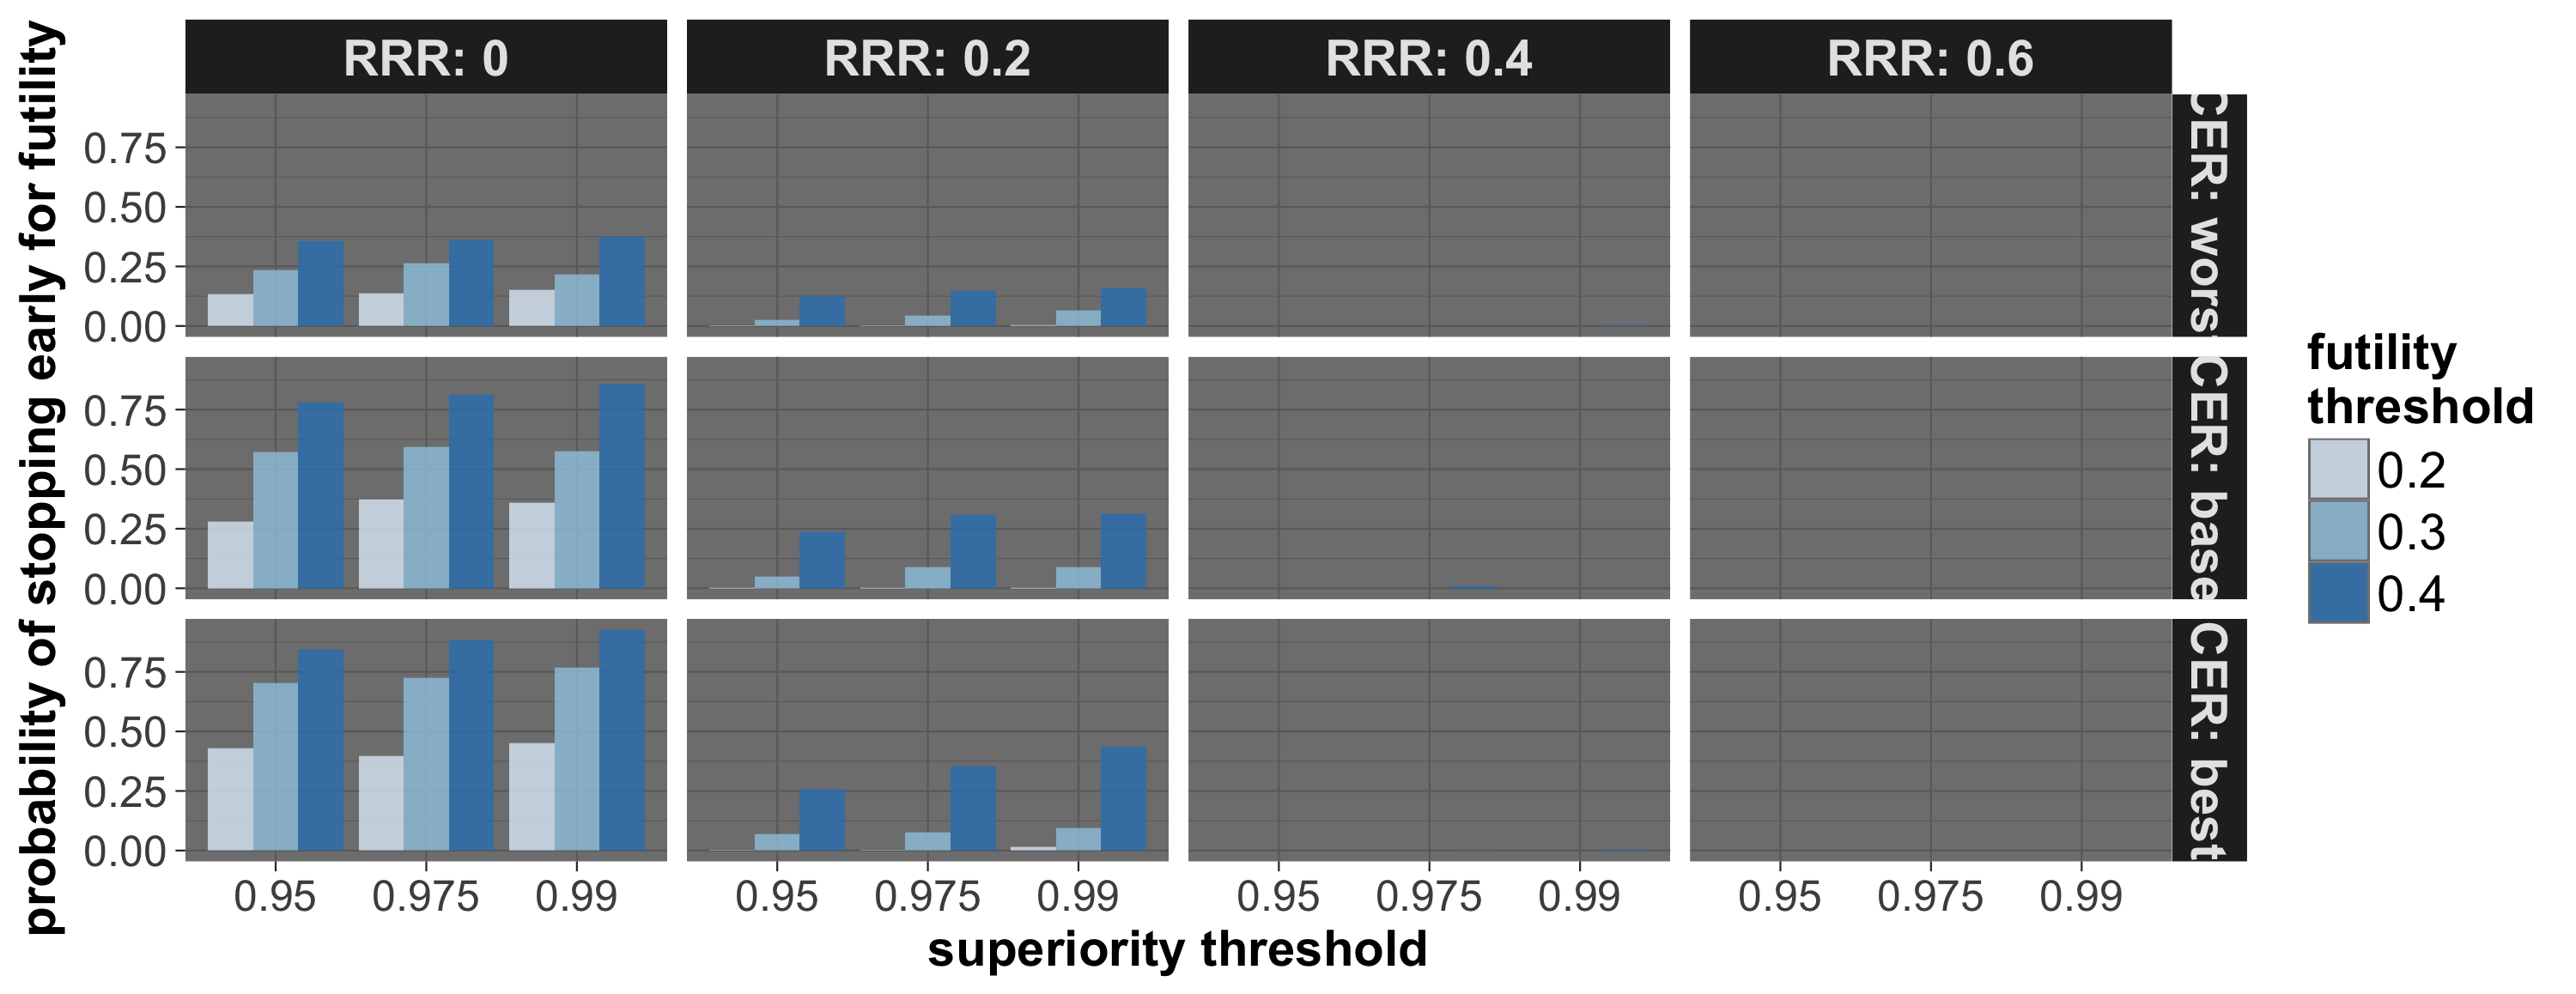
\includegraphics{../plots/stop_p1_new/early_fut_sim_05_stopp1_new.png}
  \end{subfigure}
  \begin{subfigure}{0.8\textwidth}
    \centering
    \caption{}
    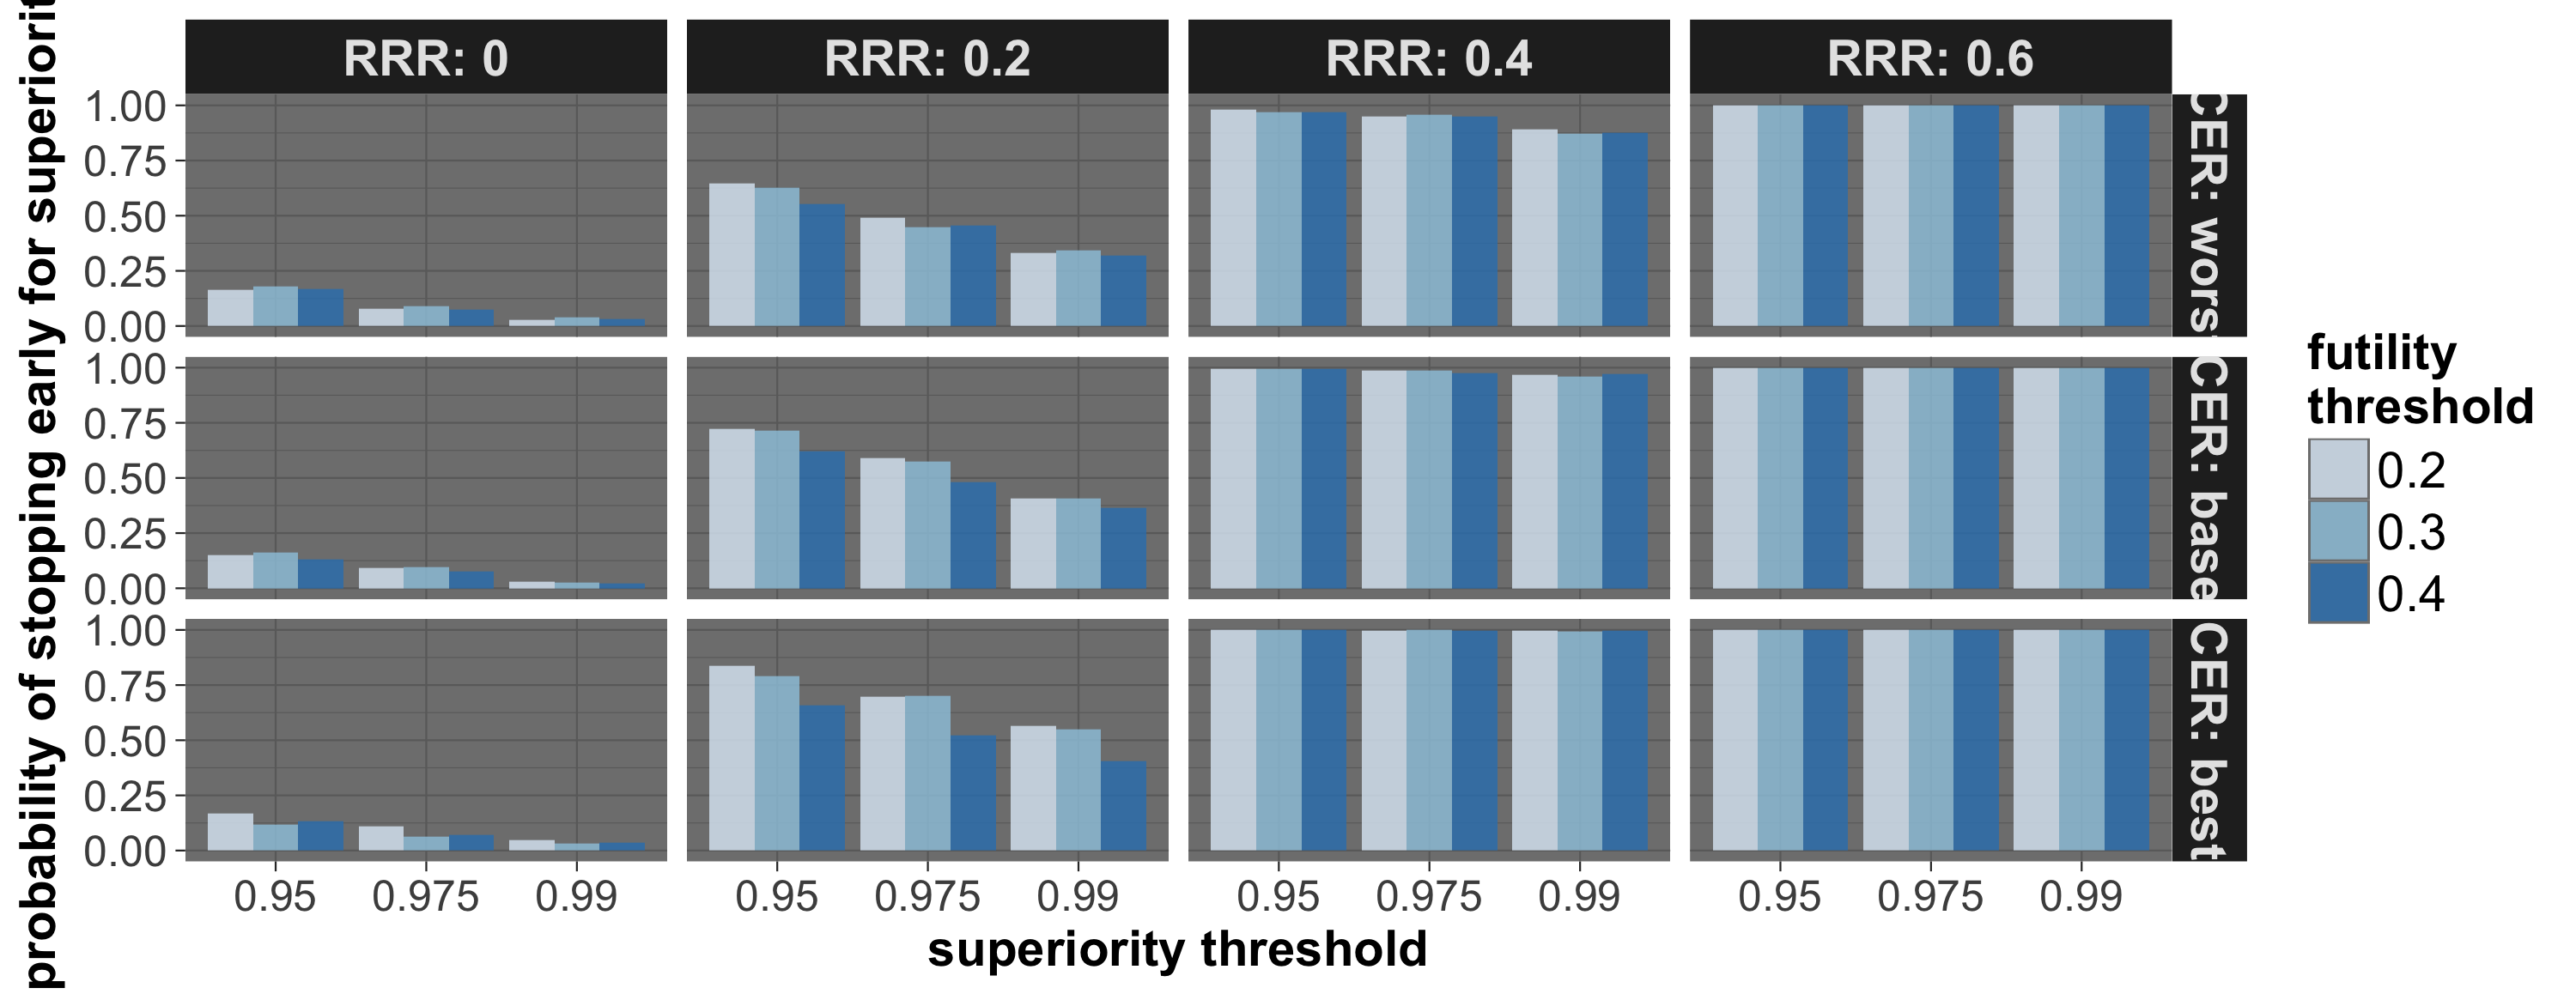
\includegraphics{../plots/stop_p1_new/early_sup_sim_05_stopp1_new.png}
  \end{subfigure}
\end{figure}

\hypertarget{p-values-at-trial-termination-when-a-true-effect-exists}{%
\paragraph{P-values at trial termination when a true effect
exists}\label{p-values-at-trial-termination-when-a-true-effect-exists}}

Figure 8 presents the categorical distribution of p-values
(\textless{}5\%, 5-10\%, or \textgreater{}10\%) upon trial termination
(stopping early or reaching max. allowed sample size). Figure 9(a) and
9(b) presents the divide of p-values when stopping for futility (a) and
superiority (b), respectively.

The overall probability of observing a p-value less than 5\% (i.e., a
conventionally statistically significant difference) is high or close to
100\% in scenarios when RRR=40\% or 60\% across all CER scenarios for
outcomes p1 and p2. Outcome s has a greater proportion of p-values being
\textgreater{}10\% in these scenarios. For the true RRR=20\%, p-values
less than 5\% are found in roughly 75\% of scenarios for p2, roughly
50\% for p1 and 5-25\% of s as the CER improves. A large proportion of
these scenarios found p-values \textgreater{}5\% for outcome s.

\begin{figure}
  \caption{Overall probability at trial termination that the p-value (from Fisher’s exact test) at termination of the
  trial is below 5\%, between 5\% and 10\% and greater than 10\%. The rows represent the three control even rate scenarios
  and the three columns present the three relative risk reduction scenarios.}
  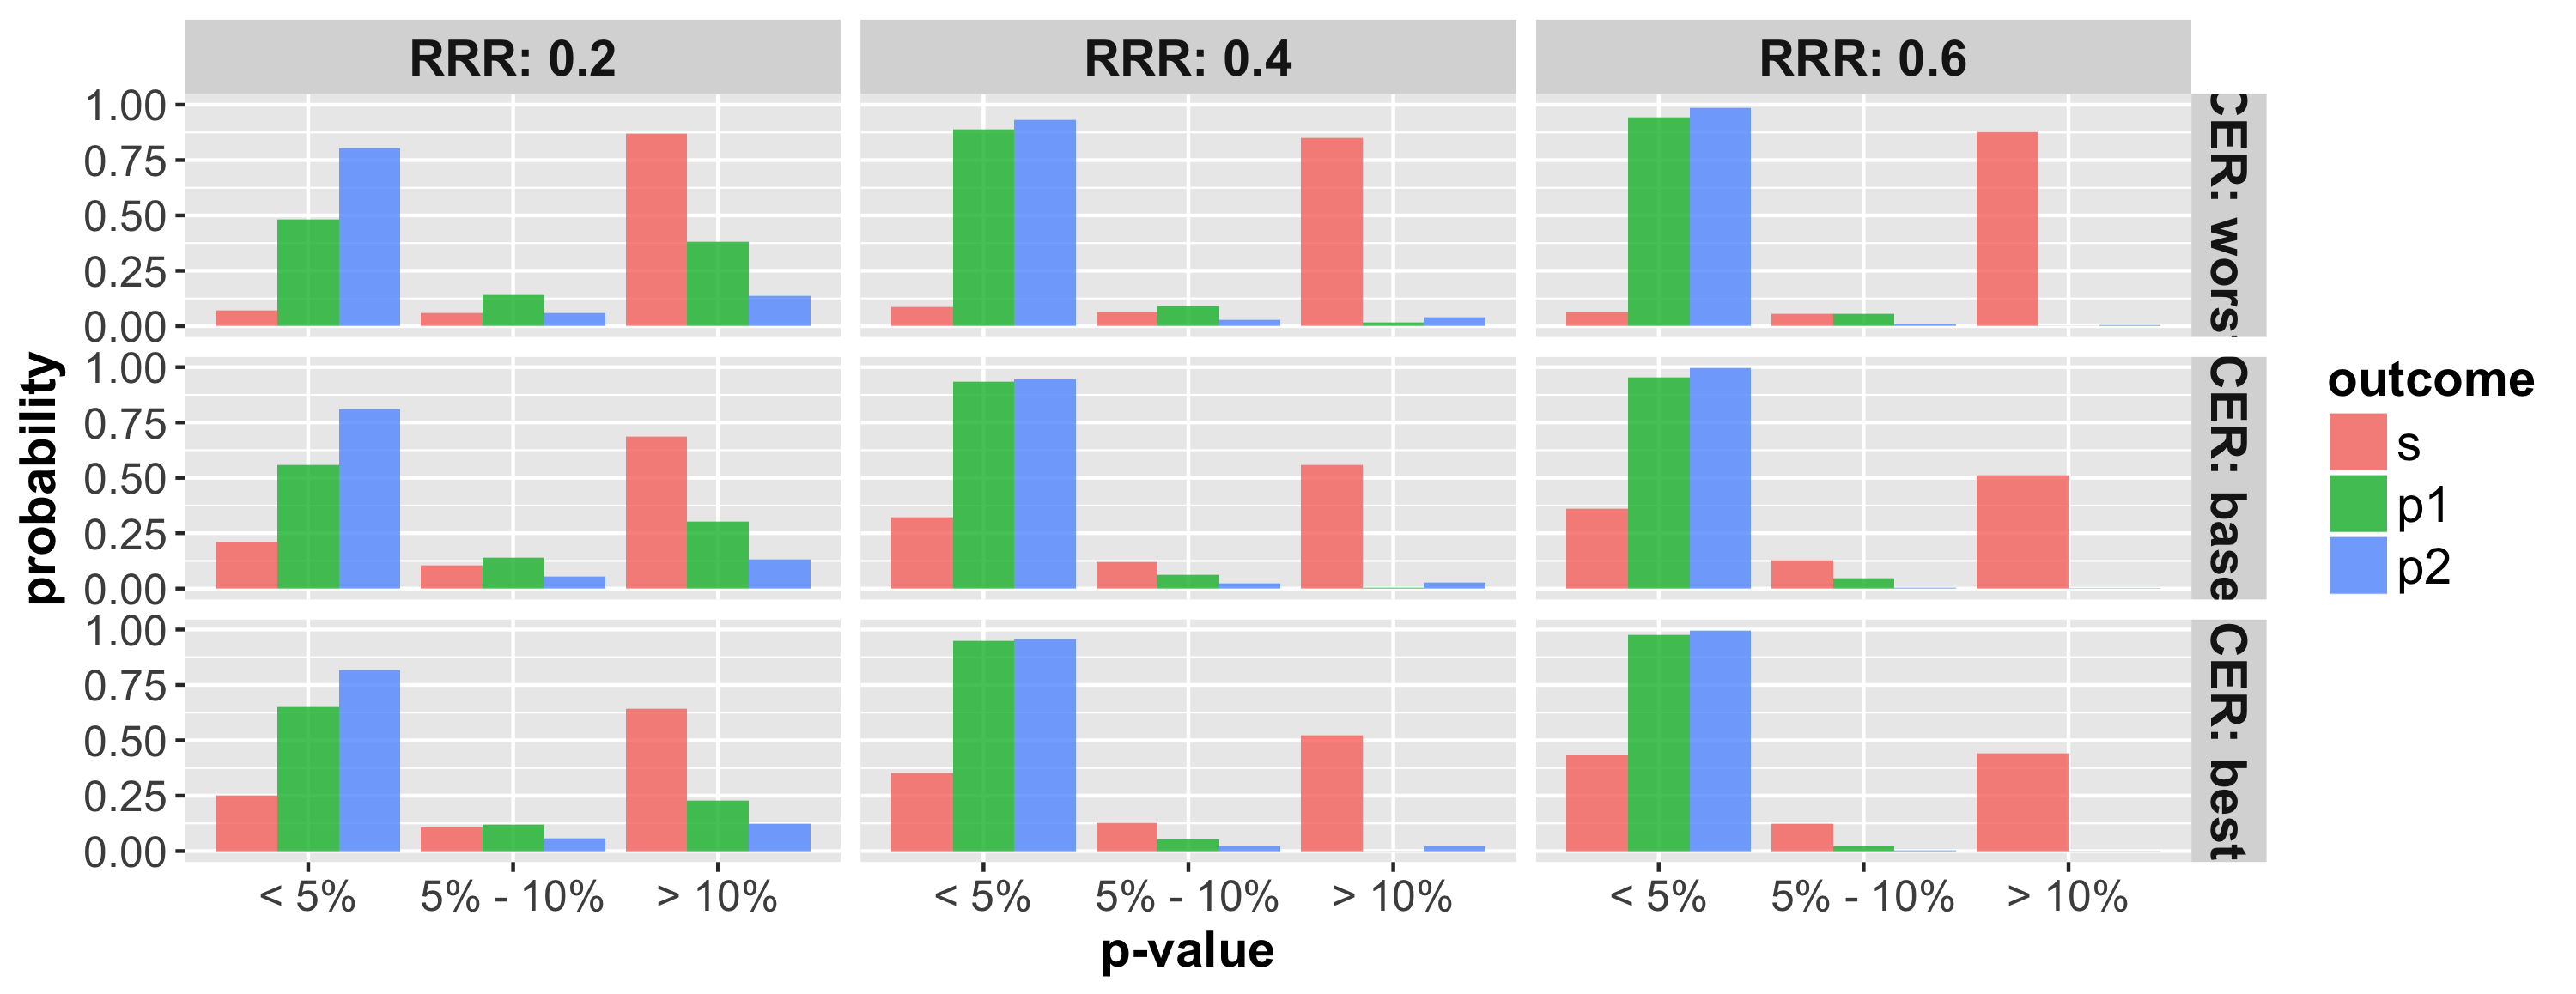
\includegraphics{../plots/stop_p1_new/pvalue_sim_05_stopp1_new.png}
\end{figure}

In the situations where the trial is stopped early for futility (shown
here for only true RRR=20\% and 40\%), the majority of p-values for
outcomes p2 are smaller than 5\%, but are greater than 10\% for outcomes
p1 and p2 when the true RRR=20\%. This and the small counts for RRR=40\%
can be explained by the low probability of stopping early for futility
under these scenarios (Figure 7(a)). When the trial is stopped for
superiority when the true RRR=40\% or 60\%, close to 100\% of all
p-values for outcomes p1 and p2 are smaller than 5\%. Under all RRR and
CER scenarios, the majority of p-values for outcomes s remain greater
than 10\%.

\begin{figure}
\centering
  \caption{Probability that the p-value (from Fisher’s exact test) at termination of the trial is below 5\%, between 5\%
  and 10\% and greater than 10\% for cases where trial was (a) stopped for futility; (b) stopped for superiority. The
  rows represent the three control even rate scenarios and the three columns present the three relative risk reduction
  scenarios. Note: the denominator in each figure is the number of simulations (not the number of trials stopped for
  futility (a) or superiority (b), and thus, the proportions do not add up to 100\% within one figure. Further, (a) and
  (b) do not include simulations where the trial went to the max. allowed sample size. The bars should be interpreted
  with respect to the relative proportion that fit in each category.}
  \begin{subfigure}{0.8\textwidth}
    \centering
    \caption{}
    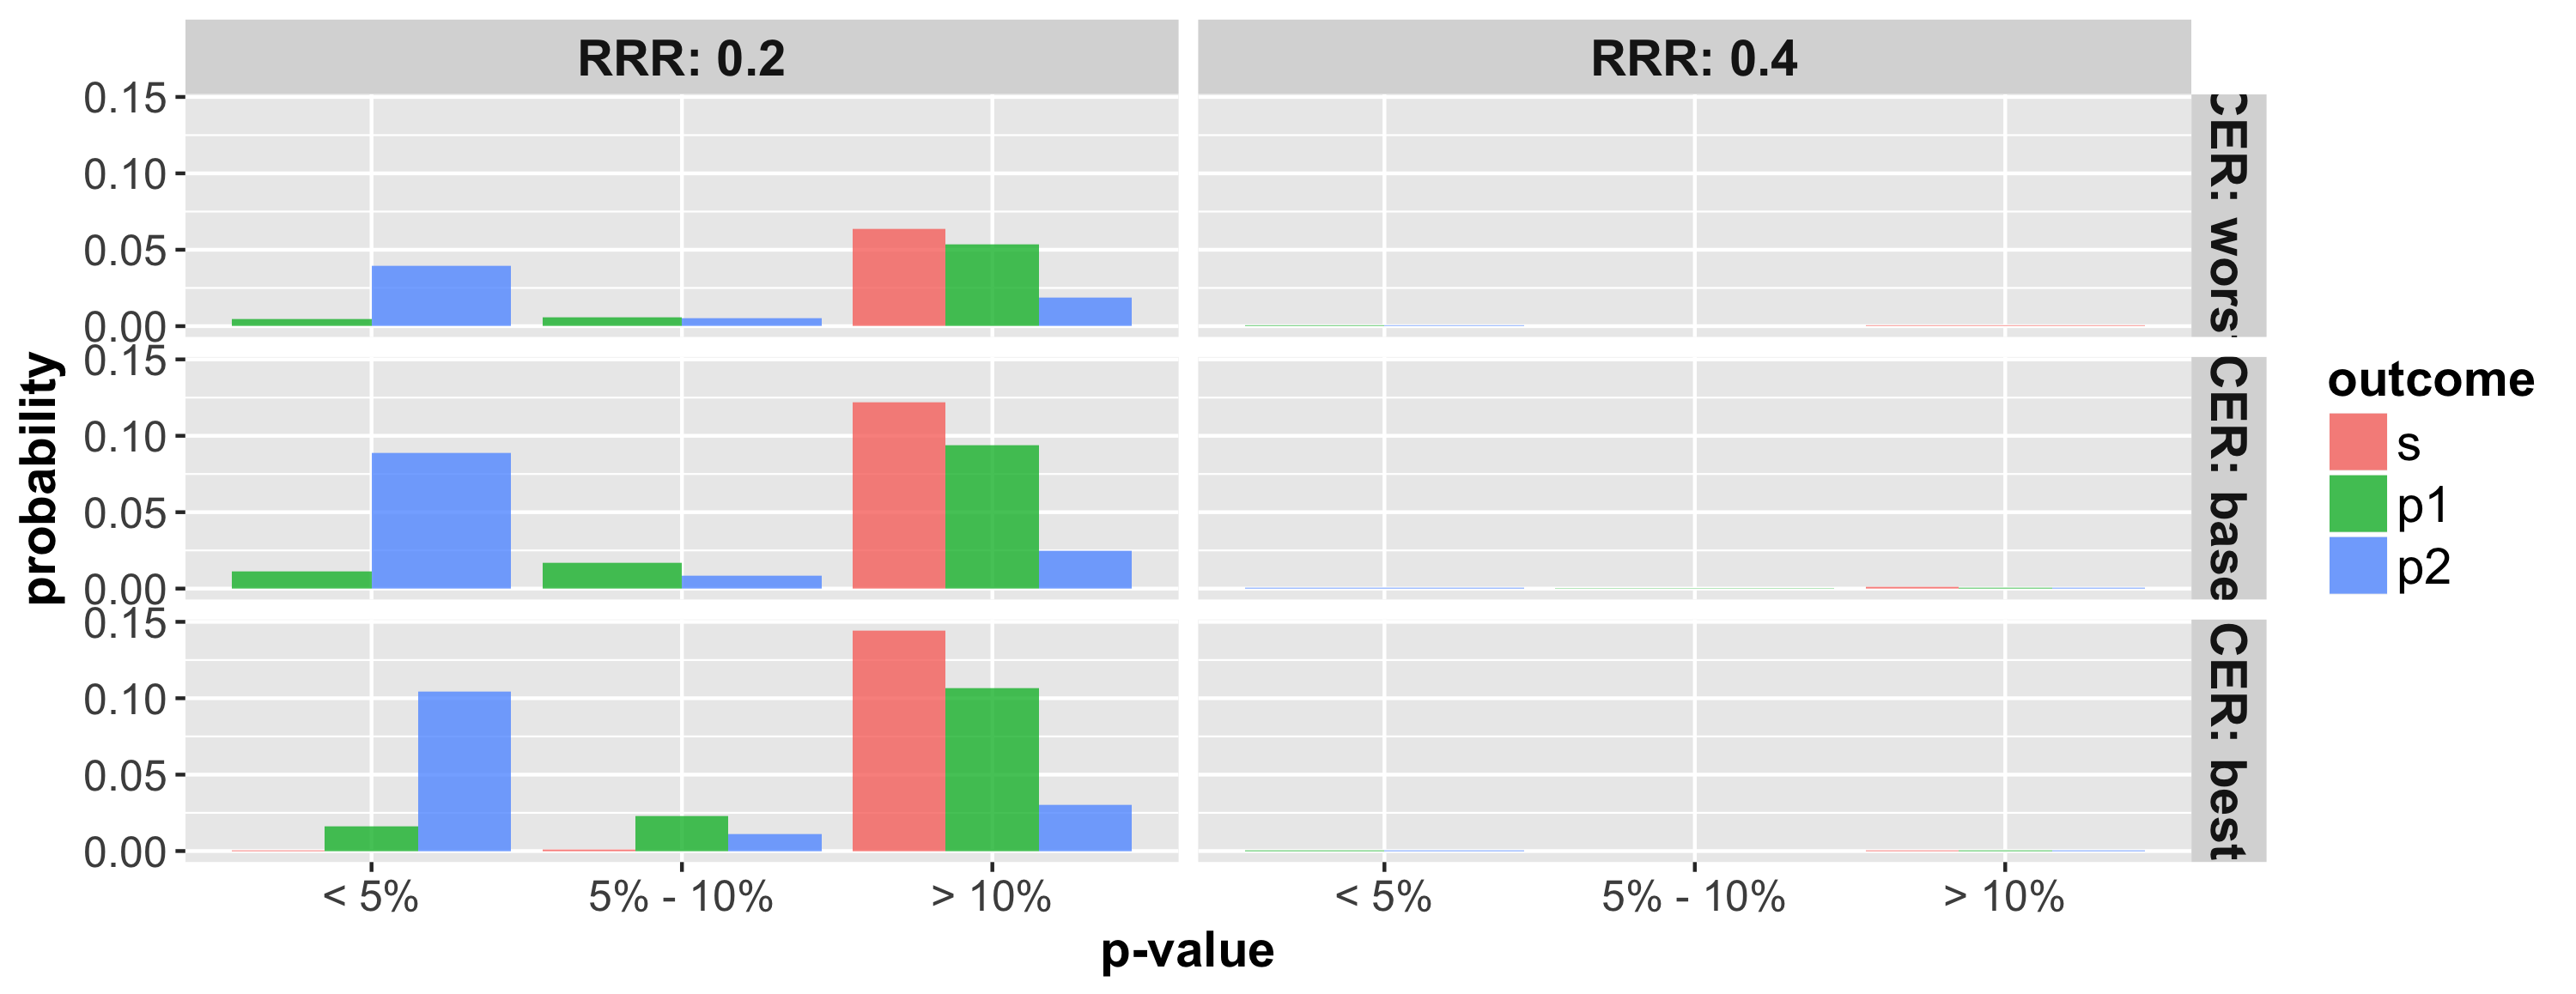
\includegraphics{../plots/stop_p1_new/pvalue_fut_sim_05_stopp1_new.png}
  \end{subfigure}
  \bigbreak
  \begin{subfigure}{0.8\textwidth}
    \centering
    \caption{}
    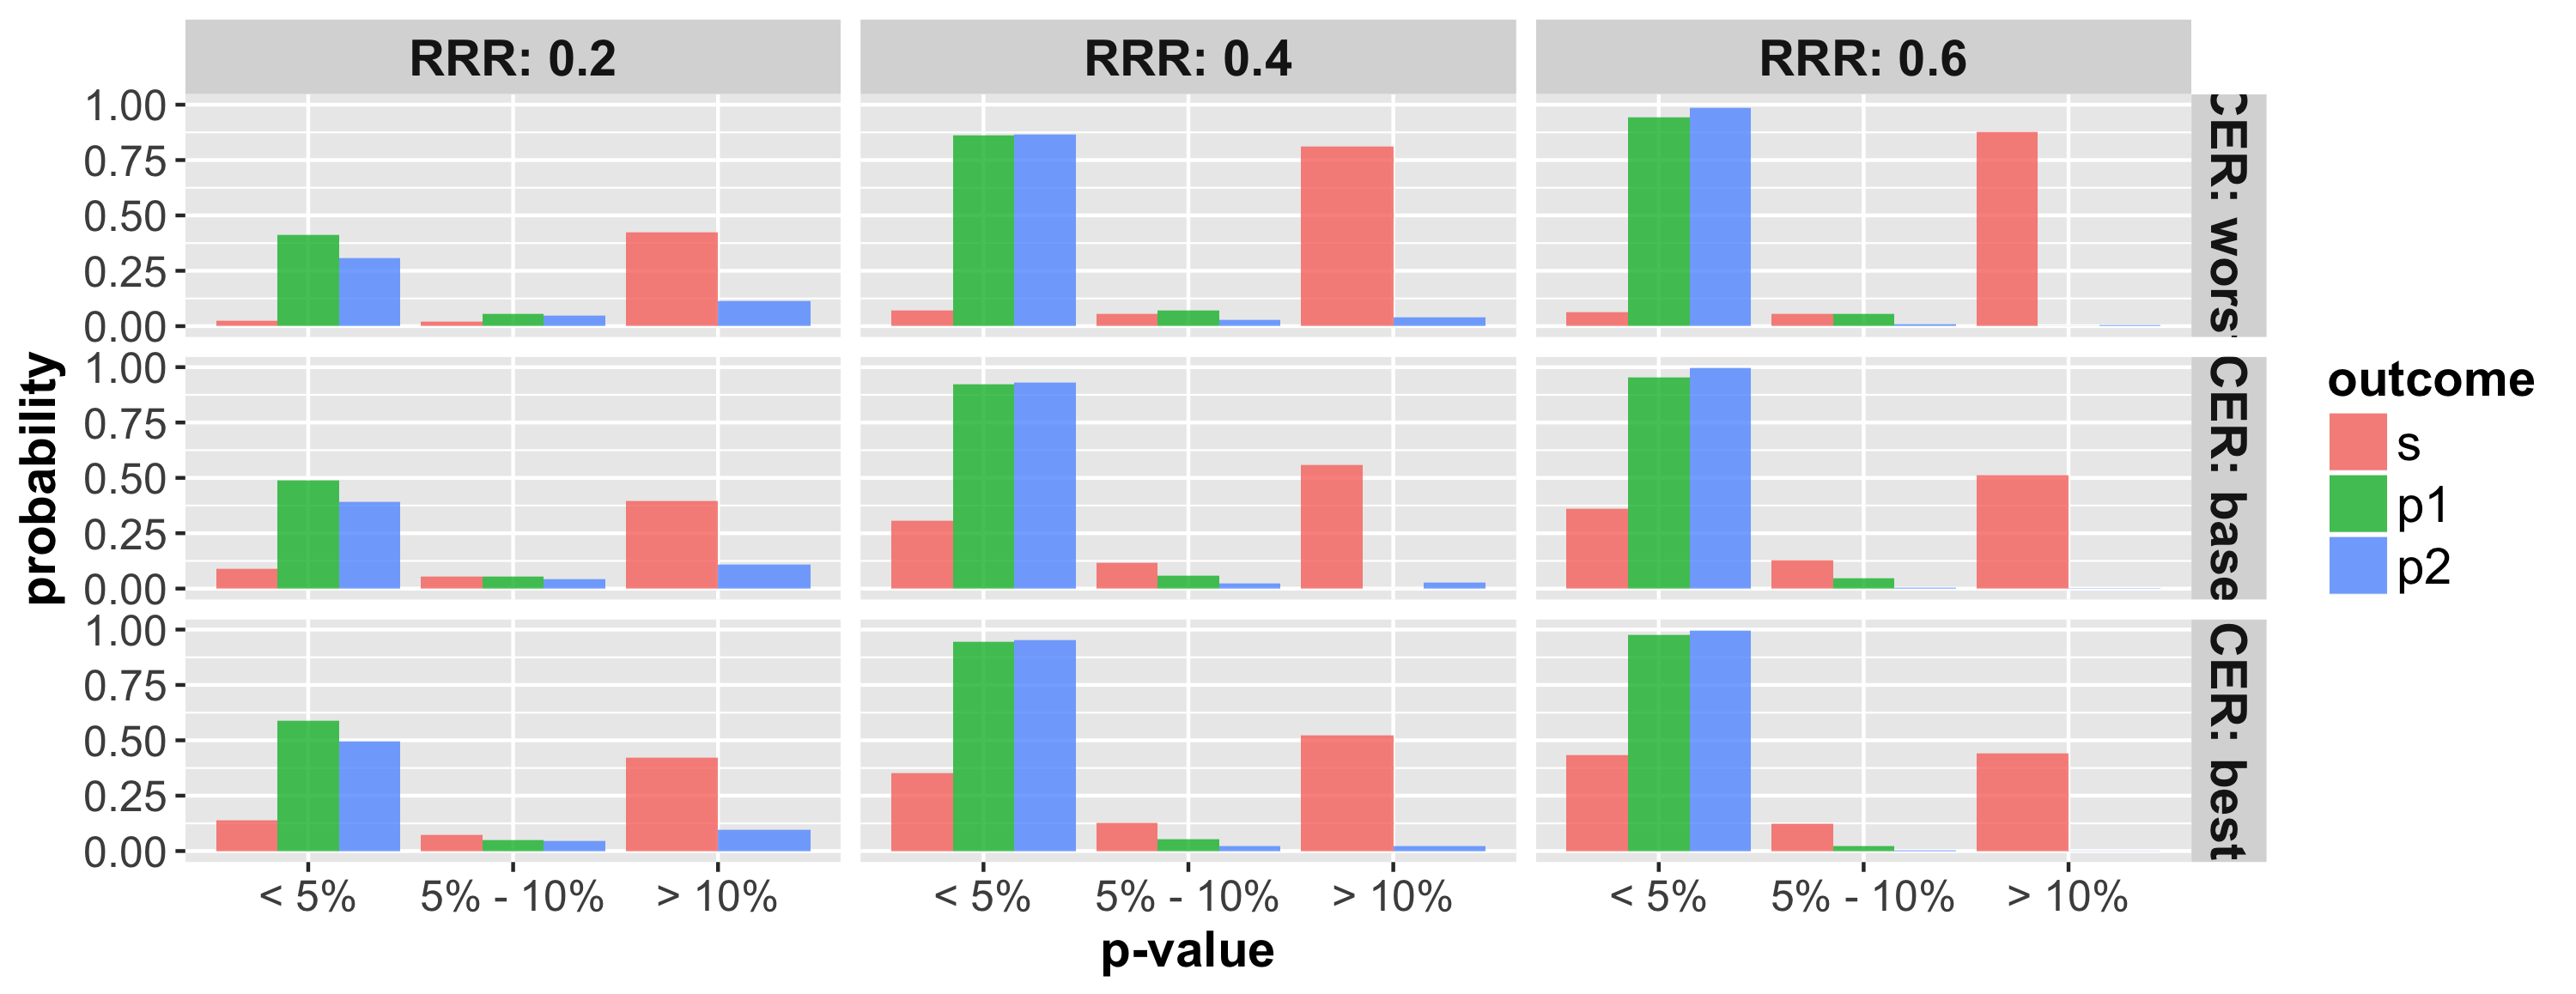
\includegraphics{../plots/stop_p1_new/pvalue_sup_sim_05_stopp1_new.png}
  \end{subfigure}
\end{figure}

\hypertarget{relative-risk-reduction-estimates-at-trial-termination}{%
\paragraph{Relative risk reduction estimates at trial
termination}\label{relative-risk-reduction-estimates-at-trial-termination}}

Figure 10 presents the distribution of relative risk reduction estimates
upon trial termination. Figure 11(a) and 11(b) present the distribution
of relative risk reduction estimates from trials stopped early for
futility and superiority, respectively. As expected, the estimates of p1
and p2 exhibit much larger precision.

\begin{figure}
  \caption{Distribution of relative risk reduction estimates (smoothed by a kernel density estimator) for the three
  control event rates (CER – rows), four relative risk reductions (RRR – columns) and the three outcomes (legend).}
  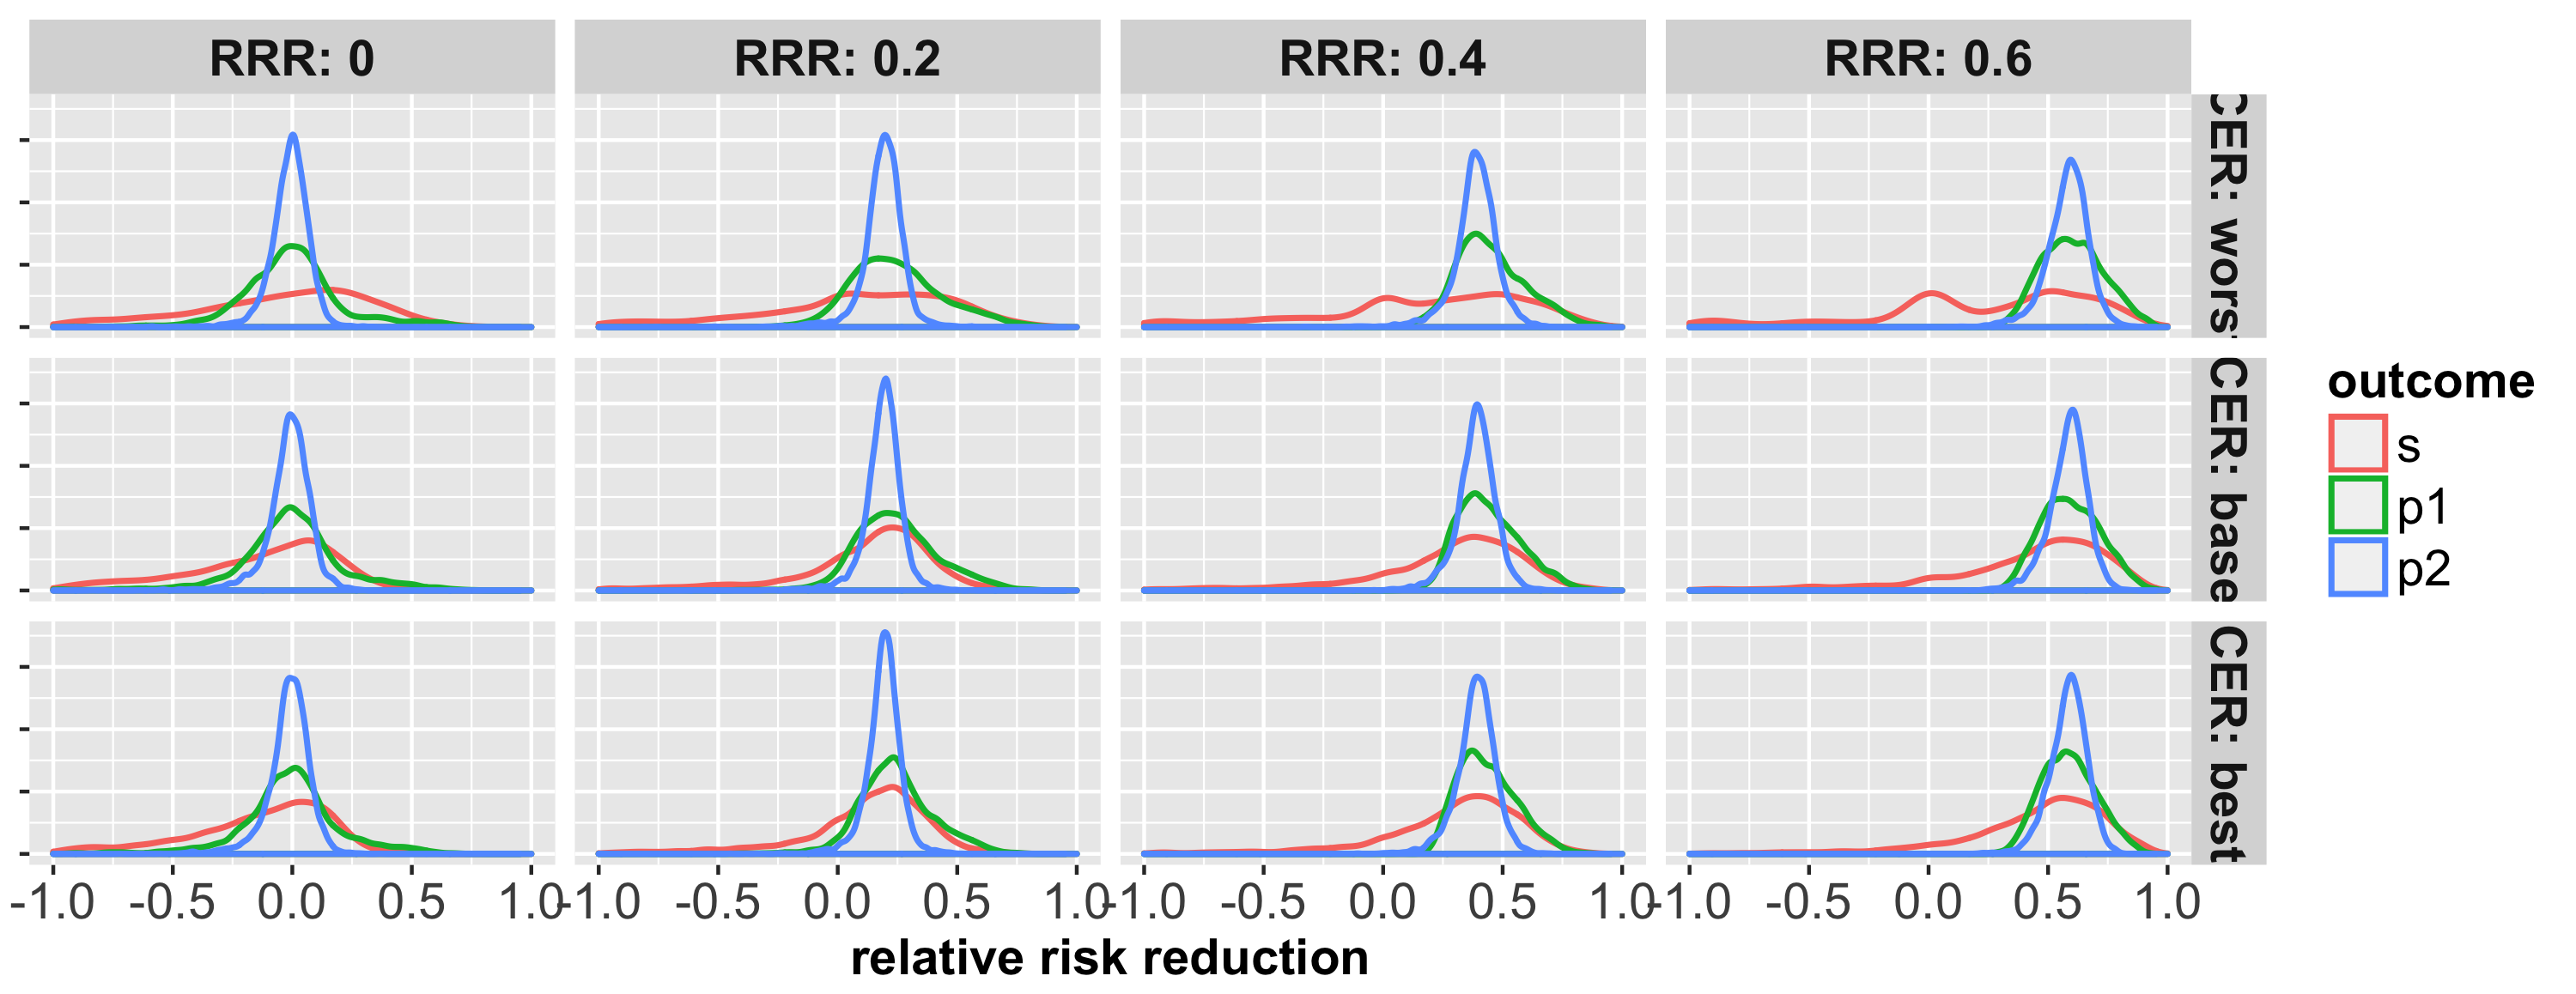
\includegraphics{../plots/stop_p1_new/RRRhat_sim_05_stopp1_new.png}
\end{figure}

When stopping for futility, outcome s incurs small to moderate downward
bias for all scenarios. For true RRR=0 and 20\% and across all CER
scenarios, both outcomes p1 and p2 show negligible bias, though p2 shows
greater precision. For RRR=40\%, outcome p1 shows less downward bias
than p2 though both are imprecise with multiple peaks. When stopping for
superiority, outcome s is very diffuse in the worst case CER scenario,
but sees its precision improve with the CER. It has marginal upward bias
when the true RRR=0 and 20\%, but shows little bias for true RRR=40\%
and 60\% for the base and best case CER scenarios. Outcome p2 has
greatest precision across all scenarios and has negligible bias. Outcome
p1 has moderate to good precision across all scenarios but has moderate
upward bias for true RRR=0 and 20\%.

\begin{figure}
\centering
  \caption{Distribution of relative risk reduction estimates after stopping early for (a) futility; (b) superiority.
  Results are presented for the three control event rates by rows, four relative risk reductions (by columns) and the
  three outcomes (legend).}
  \begin{subfigure}{0.8\textwidth}
    \centering
    \caption{}
    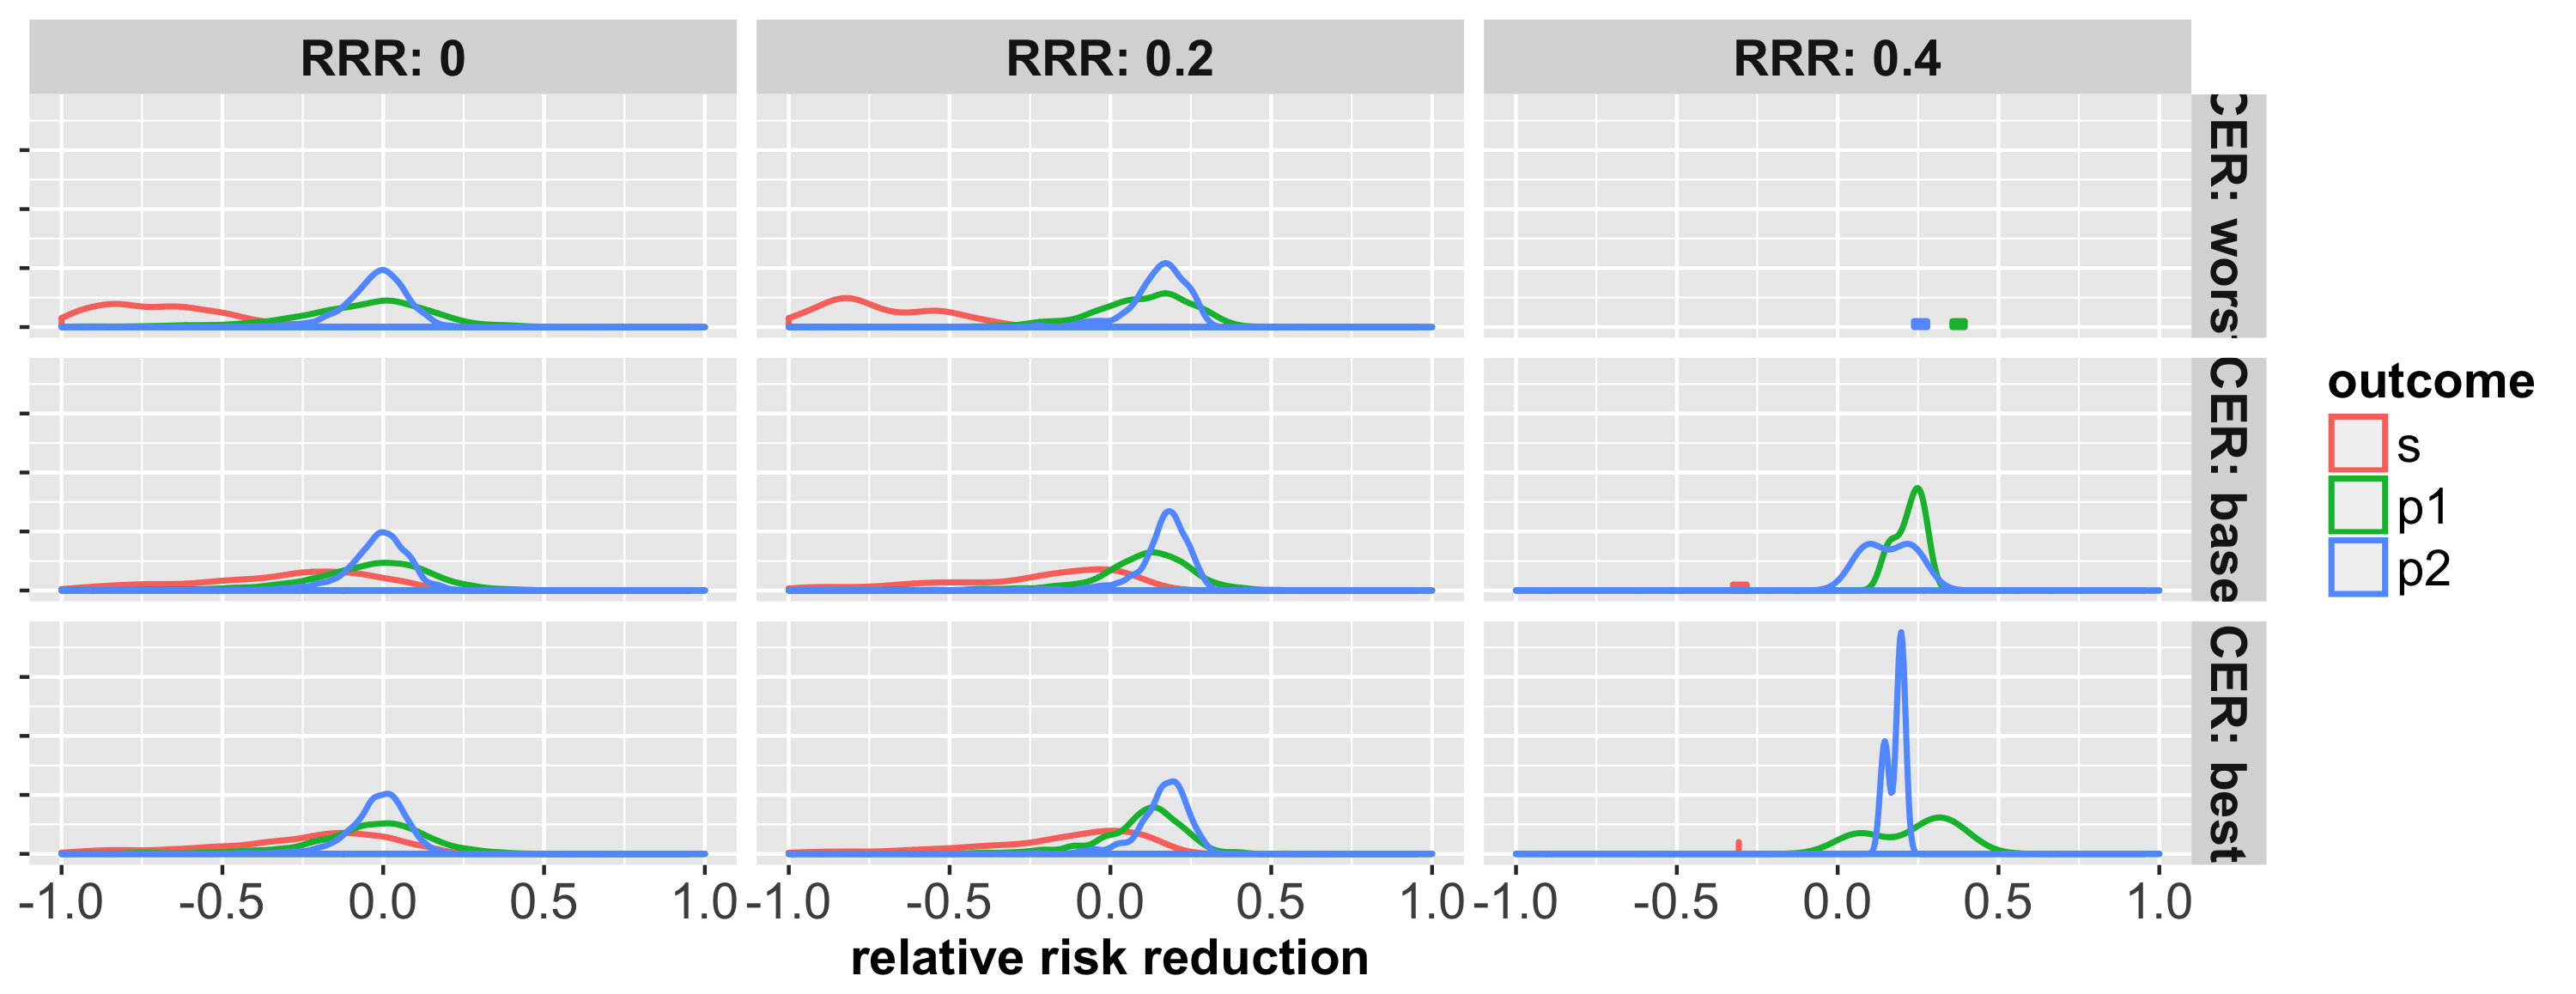
\includegraphics{../plots/stop_p1_new/RRRhat_fut_sim_05_stopp1_new.png}
  \end{subfigure}
  \bigbreak
  \begin{subfigure}{0.8\textwidth}
    \centering
    \caption{}
    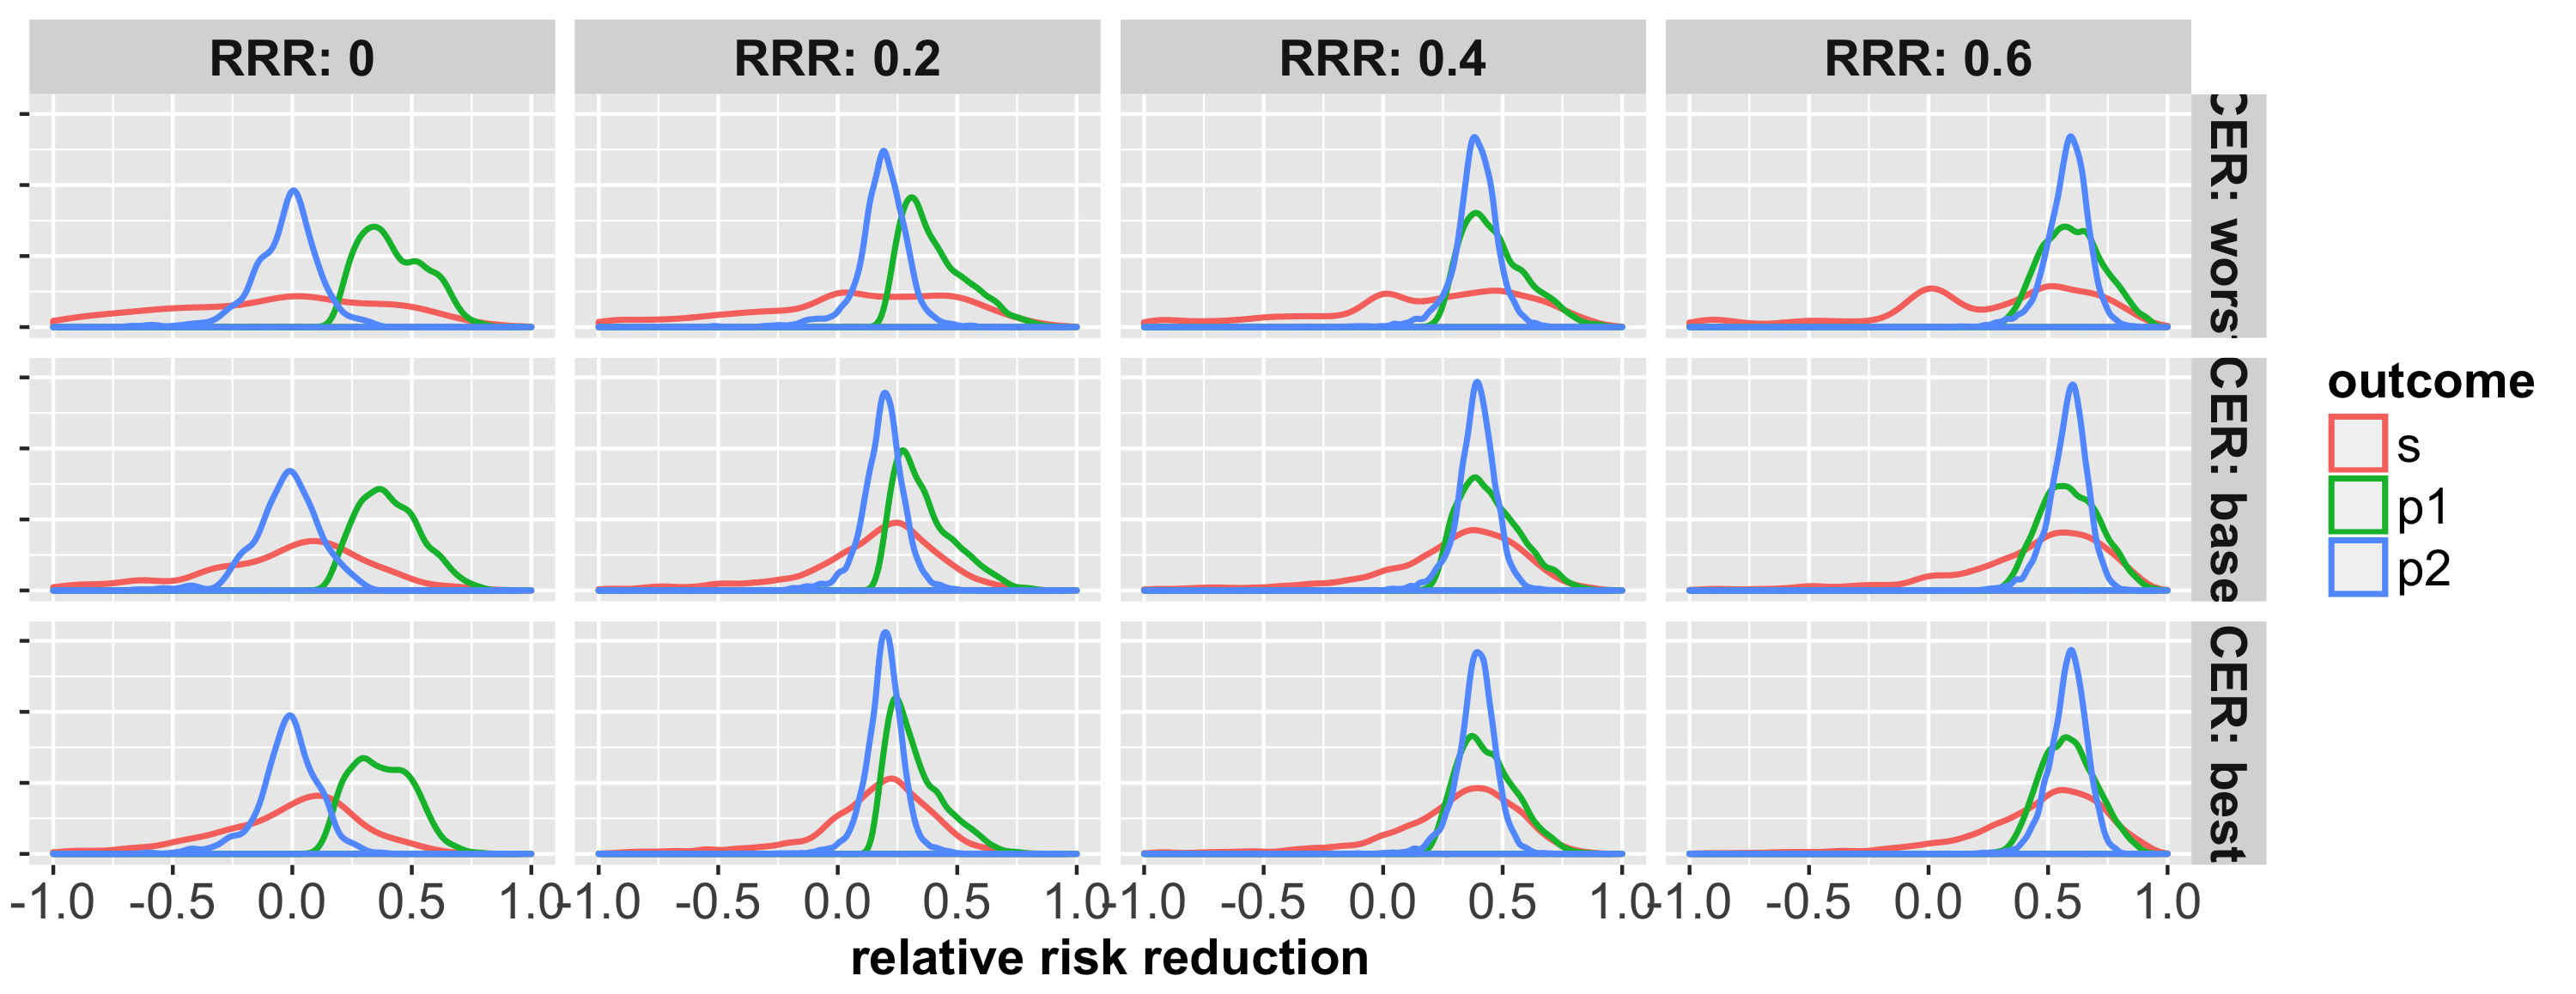
\includegraphics{../plots/stop_p1_new/RRRhat_sup_sim_05_stopp1_new.png}
  \end{subfigure}
\end{figure}

\hypertarget{multi-arm-trial-b.i.-l.p.-and-control}{%
\subsection{Multi-arm trial: B.I., L.P., and
Control}\label{multi-arm-trial-b.i.-l.p.-and-control}}

Note that pairwise comparison with control is employed and that the
three arms are not compared simultaneously. The superiority threshold
for L.P. is kept fixed at 0.99 and results are reported for the
superiority thresholds of 0.995 and 0.999 for B.I. The futility bound
was kept fixed at 0.2 and a probability threshold of 0.99 was required
to stop for futility. Both superiority and futility decisions were made
with respect to the moderately permissive outcome (p1).

\hypertarget{expected-sample-size-1}{%
\paragraph{Expected Sample Size}\label{expected-sample-size-1}}

Figure 12 presents the expected (mean) sample size at trial termination.
For true RRR=0 and RRR=20\%, expected sample sizes were consistently
high. For true of RRR=40\% and RRR=60\%, expected sample sizes were
lower and decreased as the CER improved (worst to best). Within these
RRR, the greater superiority threshold for B.I. only marginally
increased expected sample size.

\begin{figure}
  \caption{Expected sample size at trial termination. Results by control event scenarios are presented by rows. Results
  by relative risk reductions are presented by columns. Results by superiority thresholds for B.I. are presented by the
  color of the bars (see legend).}
  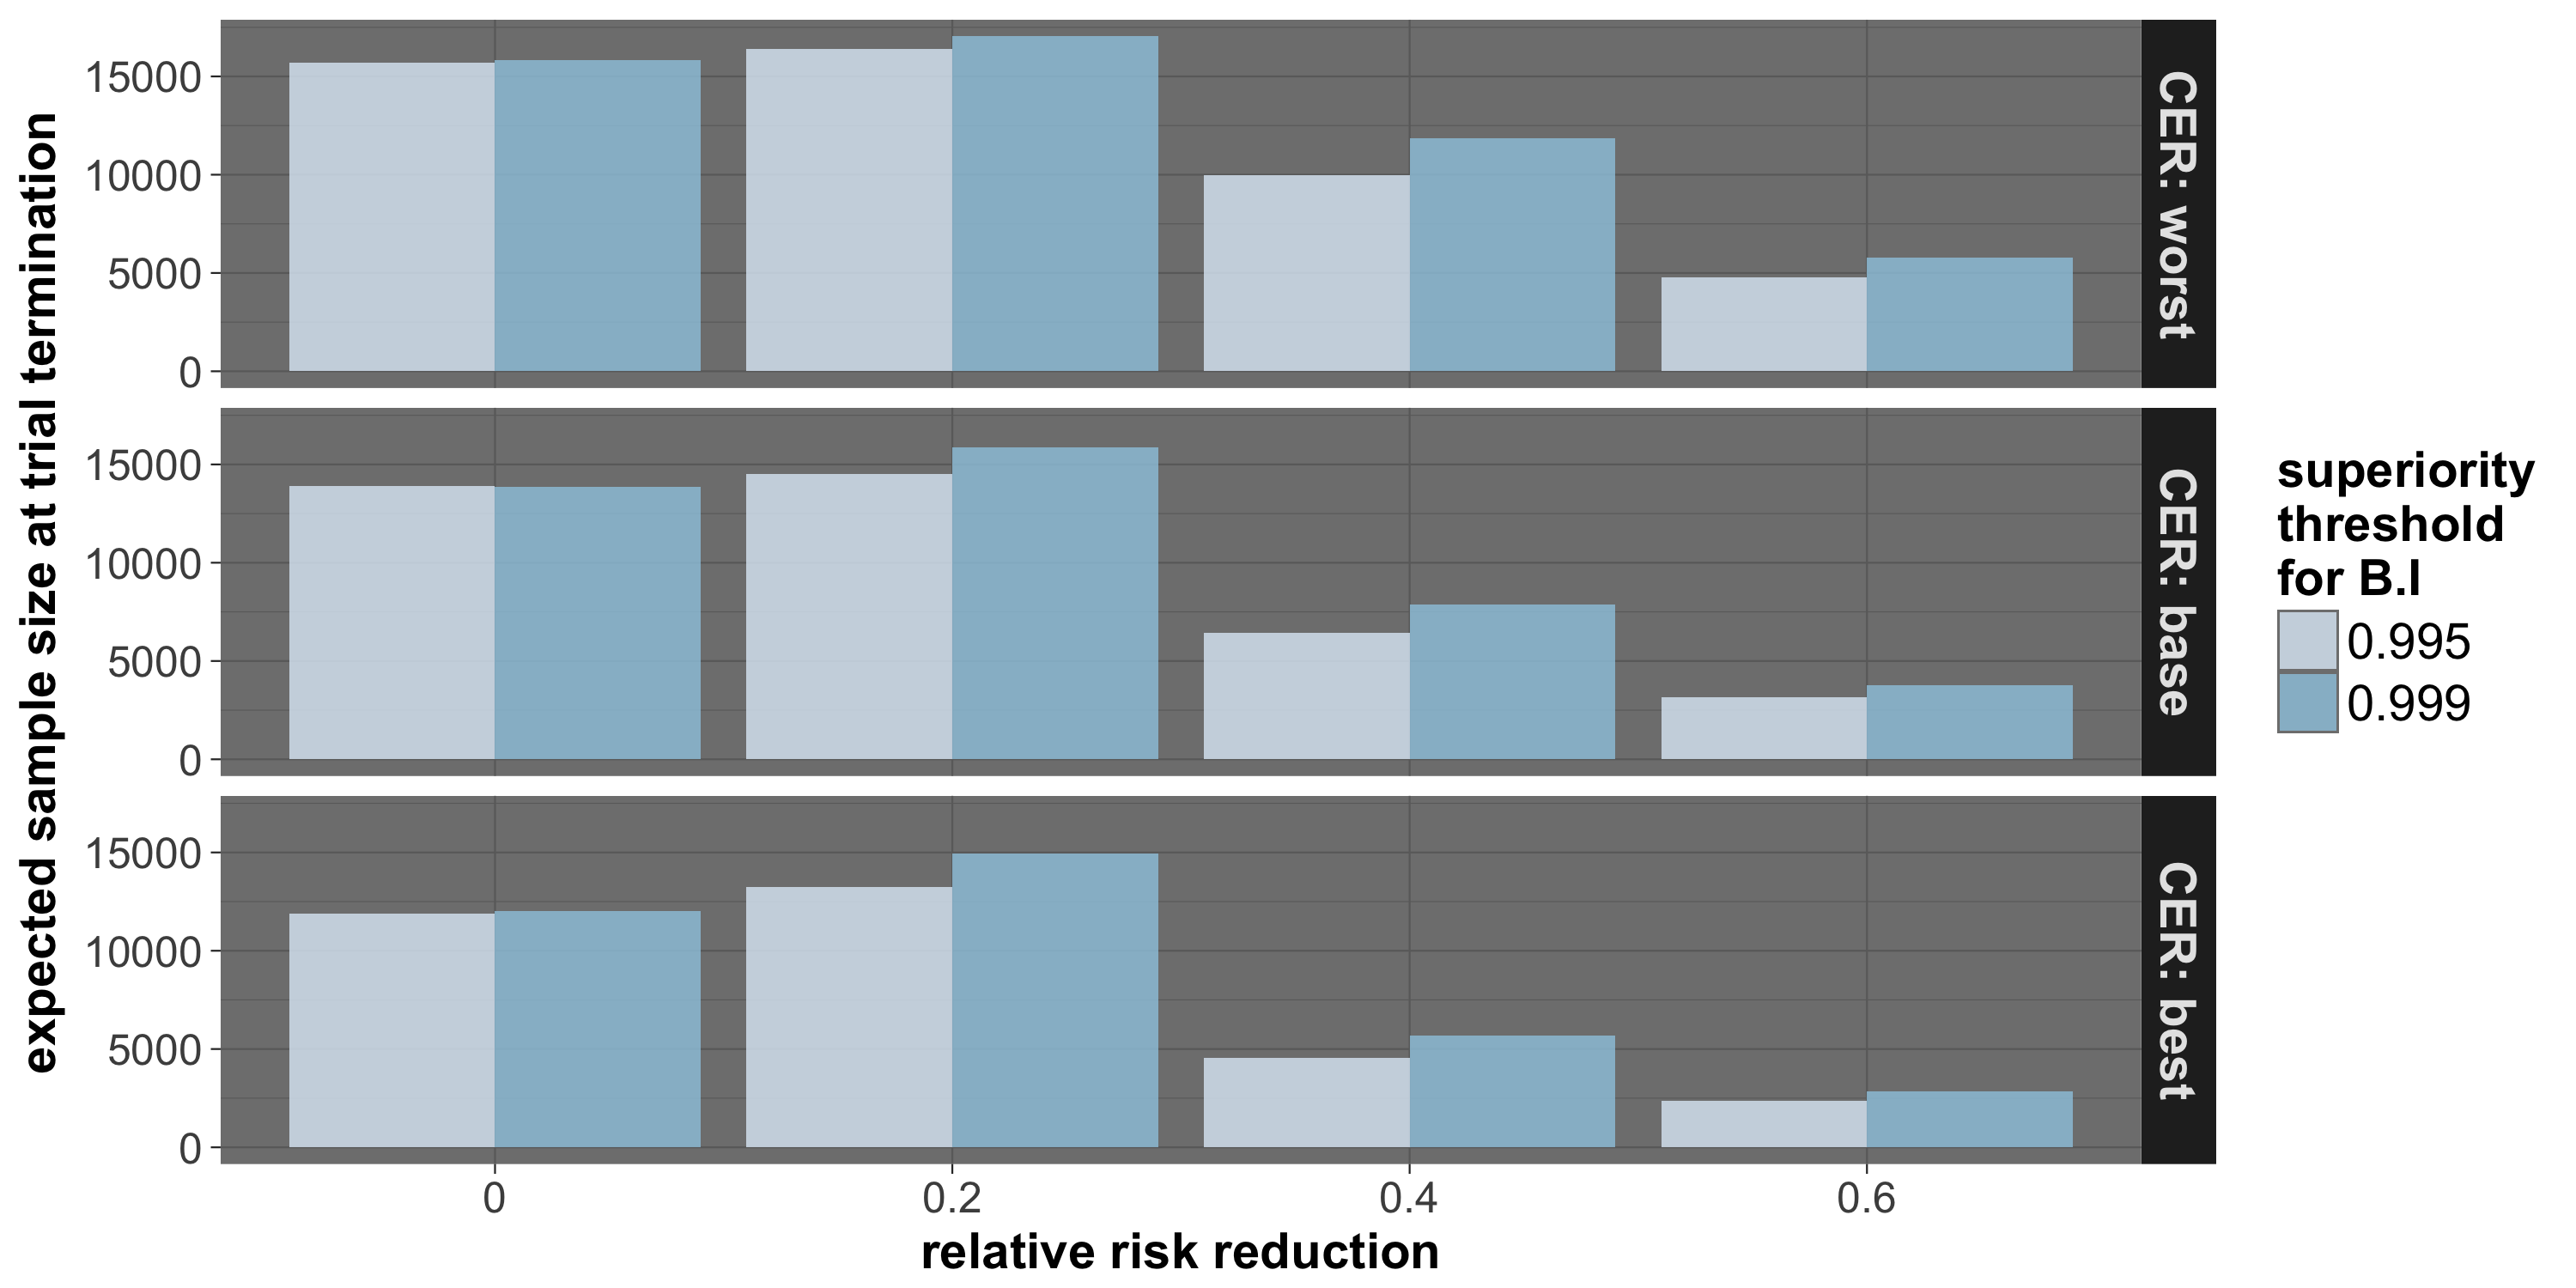
\includegraphics{../plots/3arm/ESS_3arm.png}
\end{figure}

Figure 13 shows the probability of reaching the maximum allowed sample
size of the trial. This probability was moderate to high for the true
RRR=0 and RRR=20\%, but decreased for the best case CER scenario. For
RRR=40\% and RRR=60\%, this probability was negligible for all cases
except RRR=40\% and the worst case CER scenario, where it was roughly
25\% for the highest superiority threshold.

\begin{figure}
  \caption{Probability of reaching maximum sample size for the three control event rates (CER – rows), four relative
  risk reductions (RRR – columns), and two superiority thresholds for B.I. (legend). Note that the legend and x axis labels should reflect the description given above, not as labeled on the graphic.}
  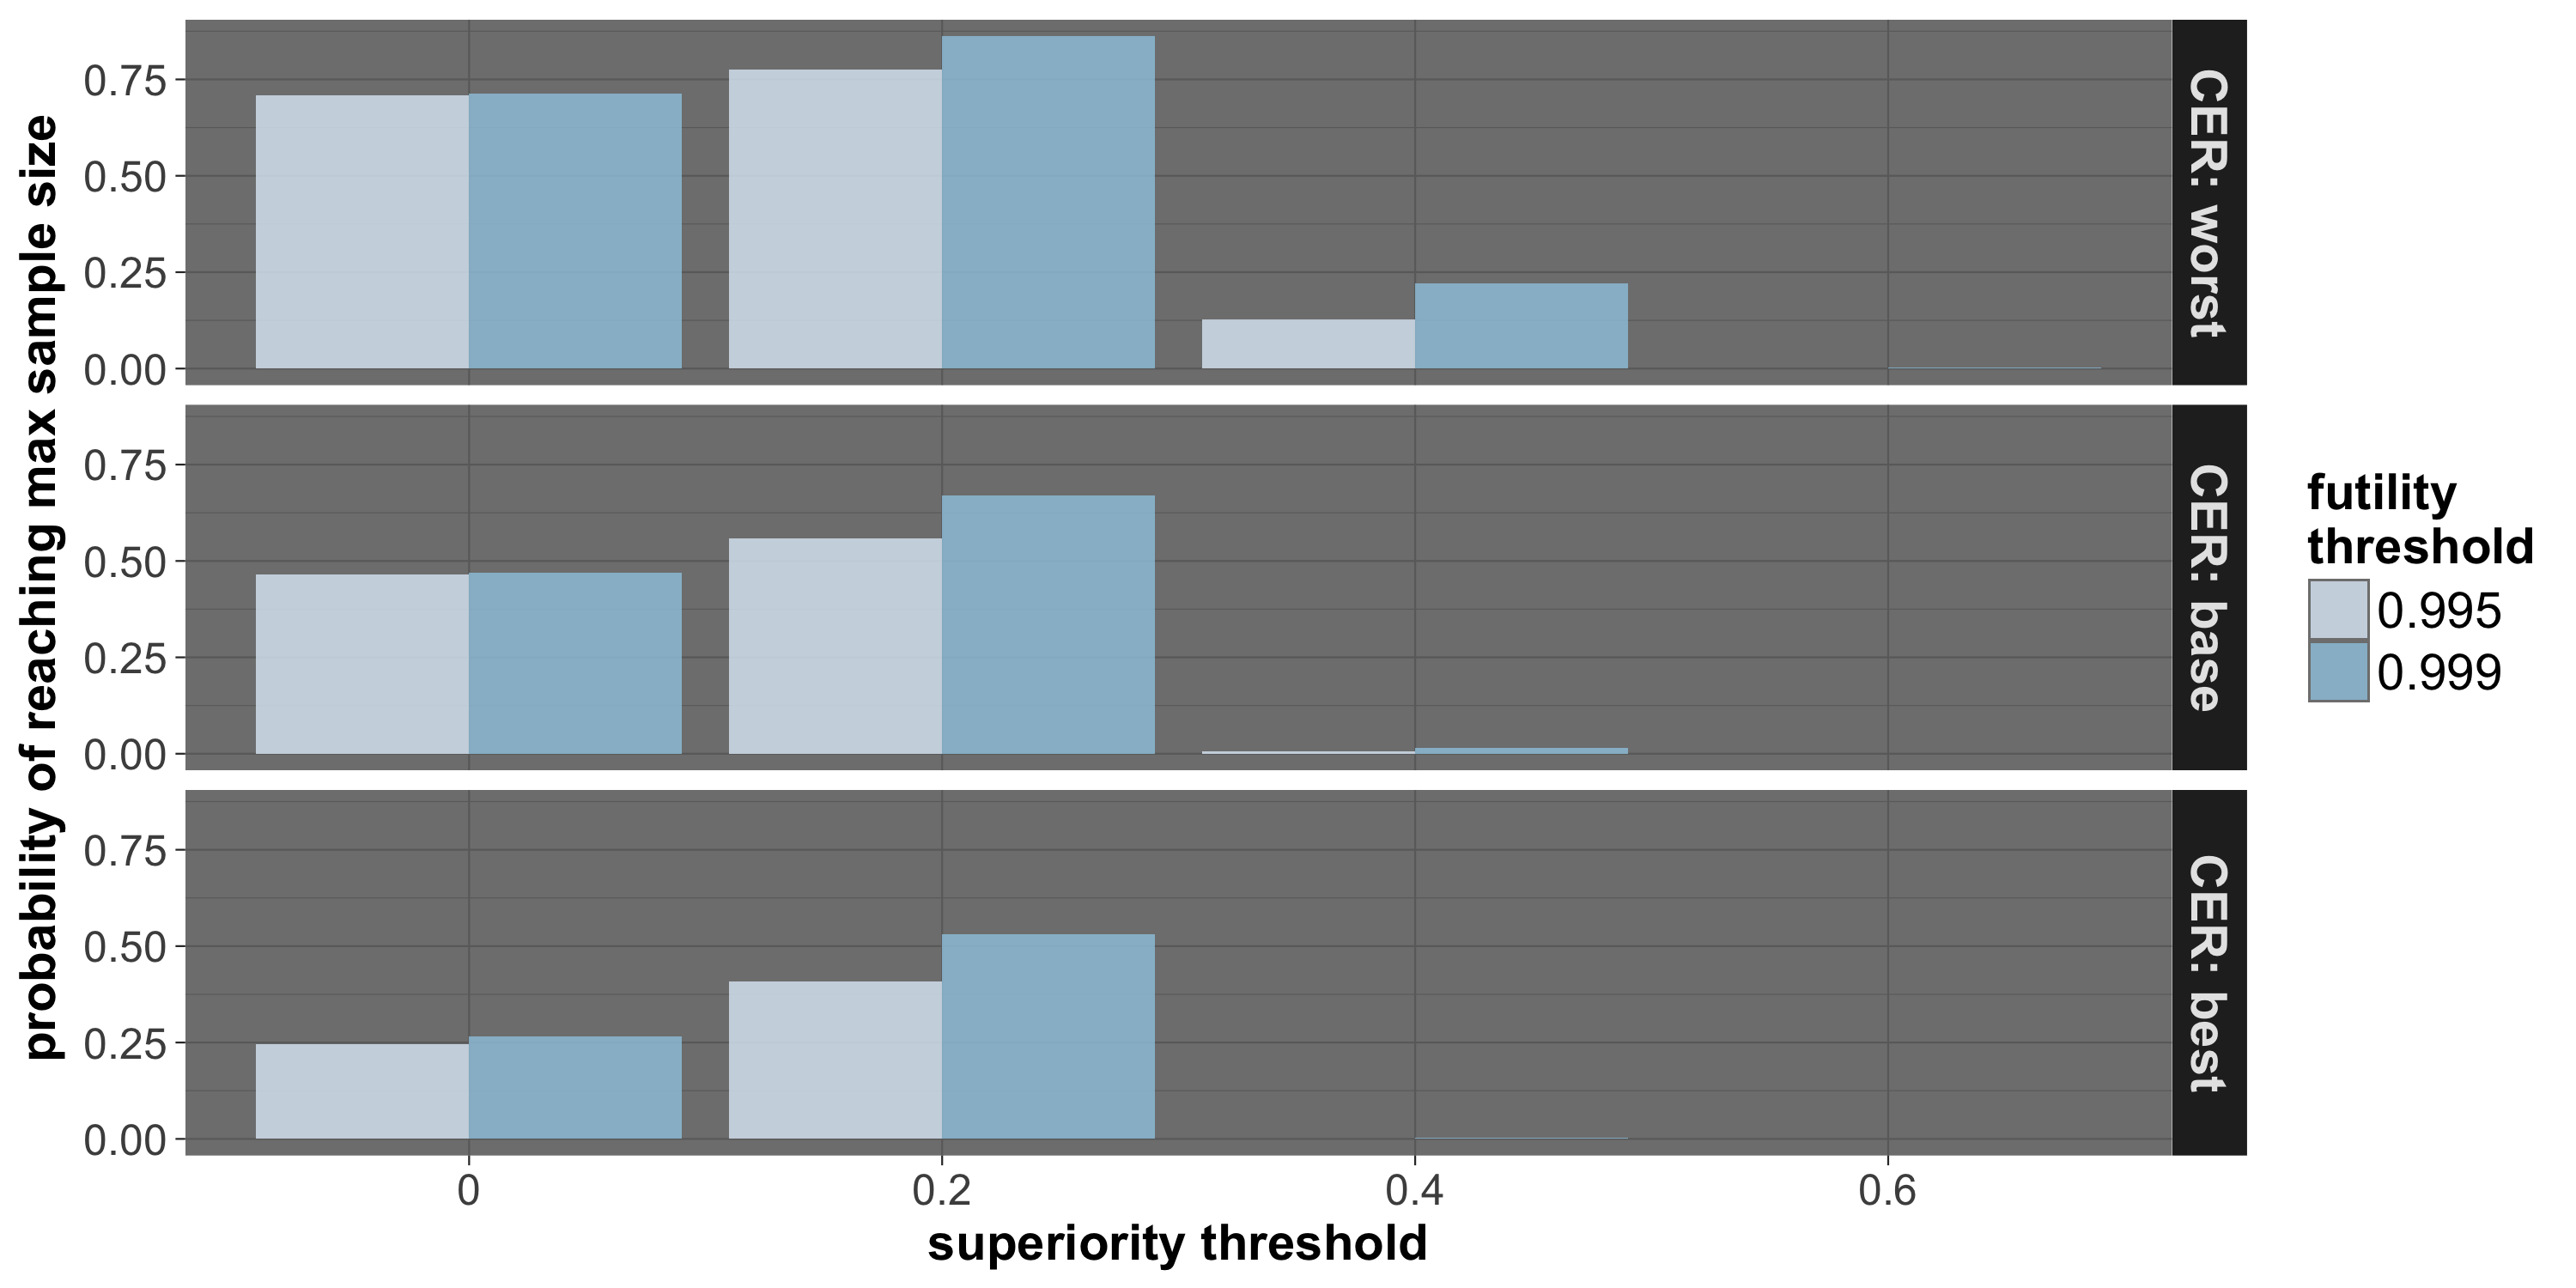
\includegraphics{../plots/3arm/reachmax_3arm.png}
\end{figure}

\hypertarget{probability-of-stopping-early-1}{%
\paragraph{Probability of Stopping
Early}\label{probability-of-stopping-early-1}}

The probability of stopping early was obtained overall, for superiority
and for futility. Figure 14 displays the overall probability of stopping
early, Figure 15 displays the probability of stopping early for futility
((a) B.I., (b) L.P.) and figure 16 displays the probability of stopping
early for superiority ((a) B.I., (b) L.P.). The overall probability of
stopping early is strongly positively correlated with the CER and RRR,
being nearly certain for RRR=40\% and RRR=60\%.

\begin{figure}
  \caption{Probability of stopping early for the three control event rates (CER – rows), four relative risk reductions
  (RRR – columns), and two superiority thresholds for B.I. (legend).}
  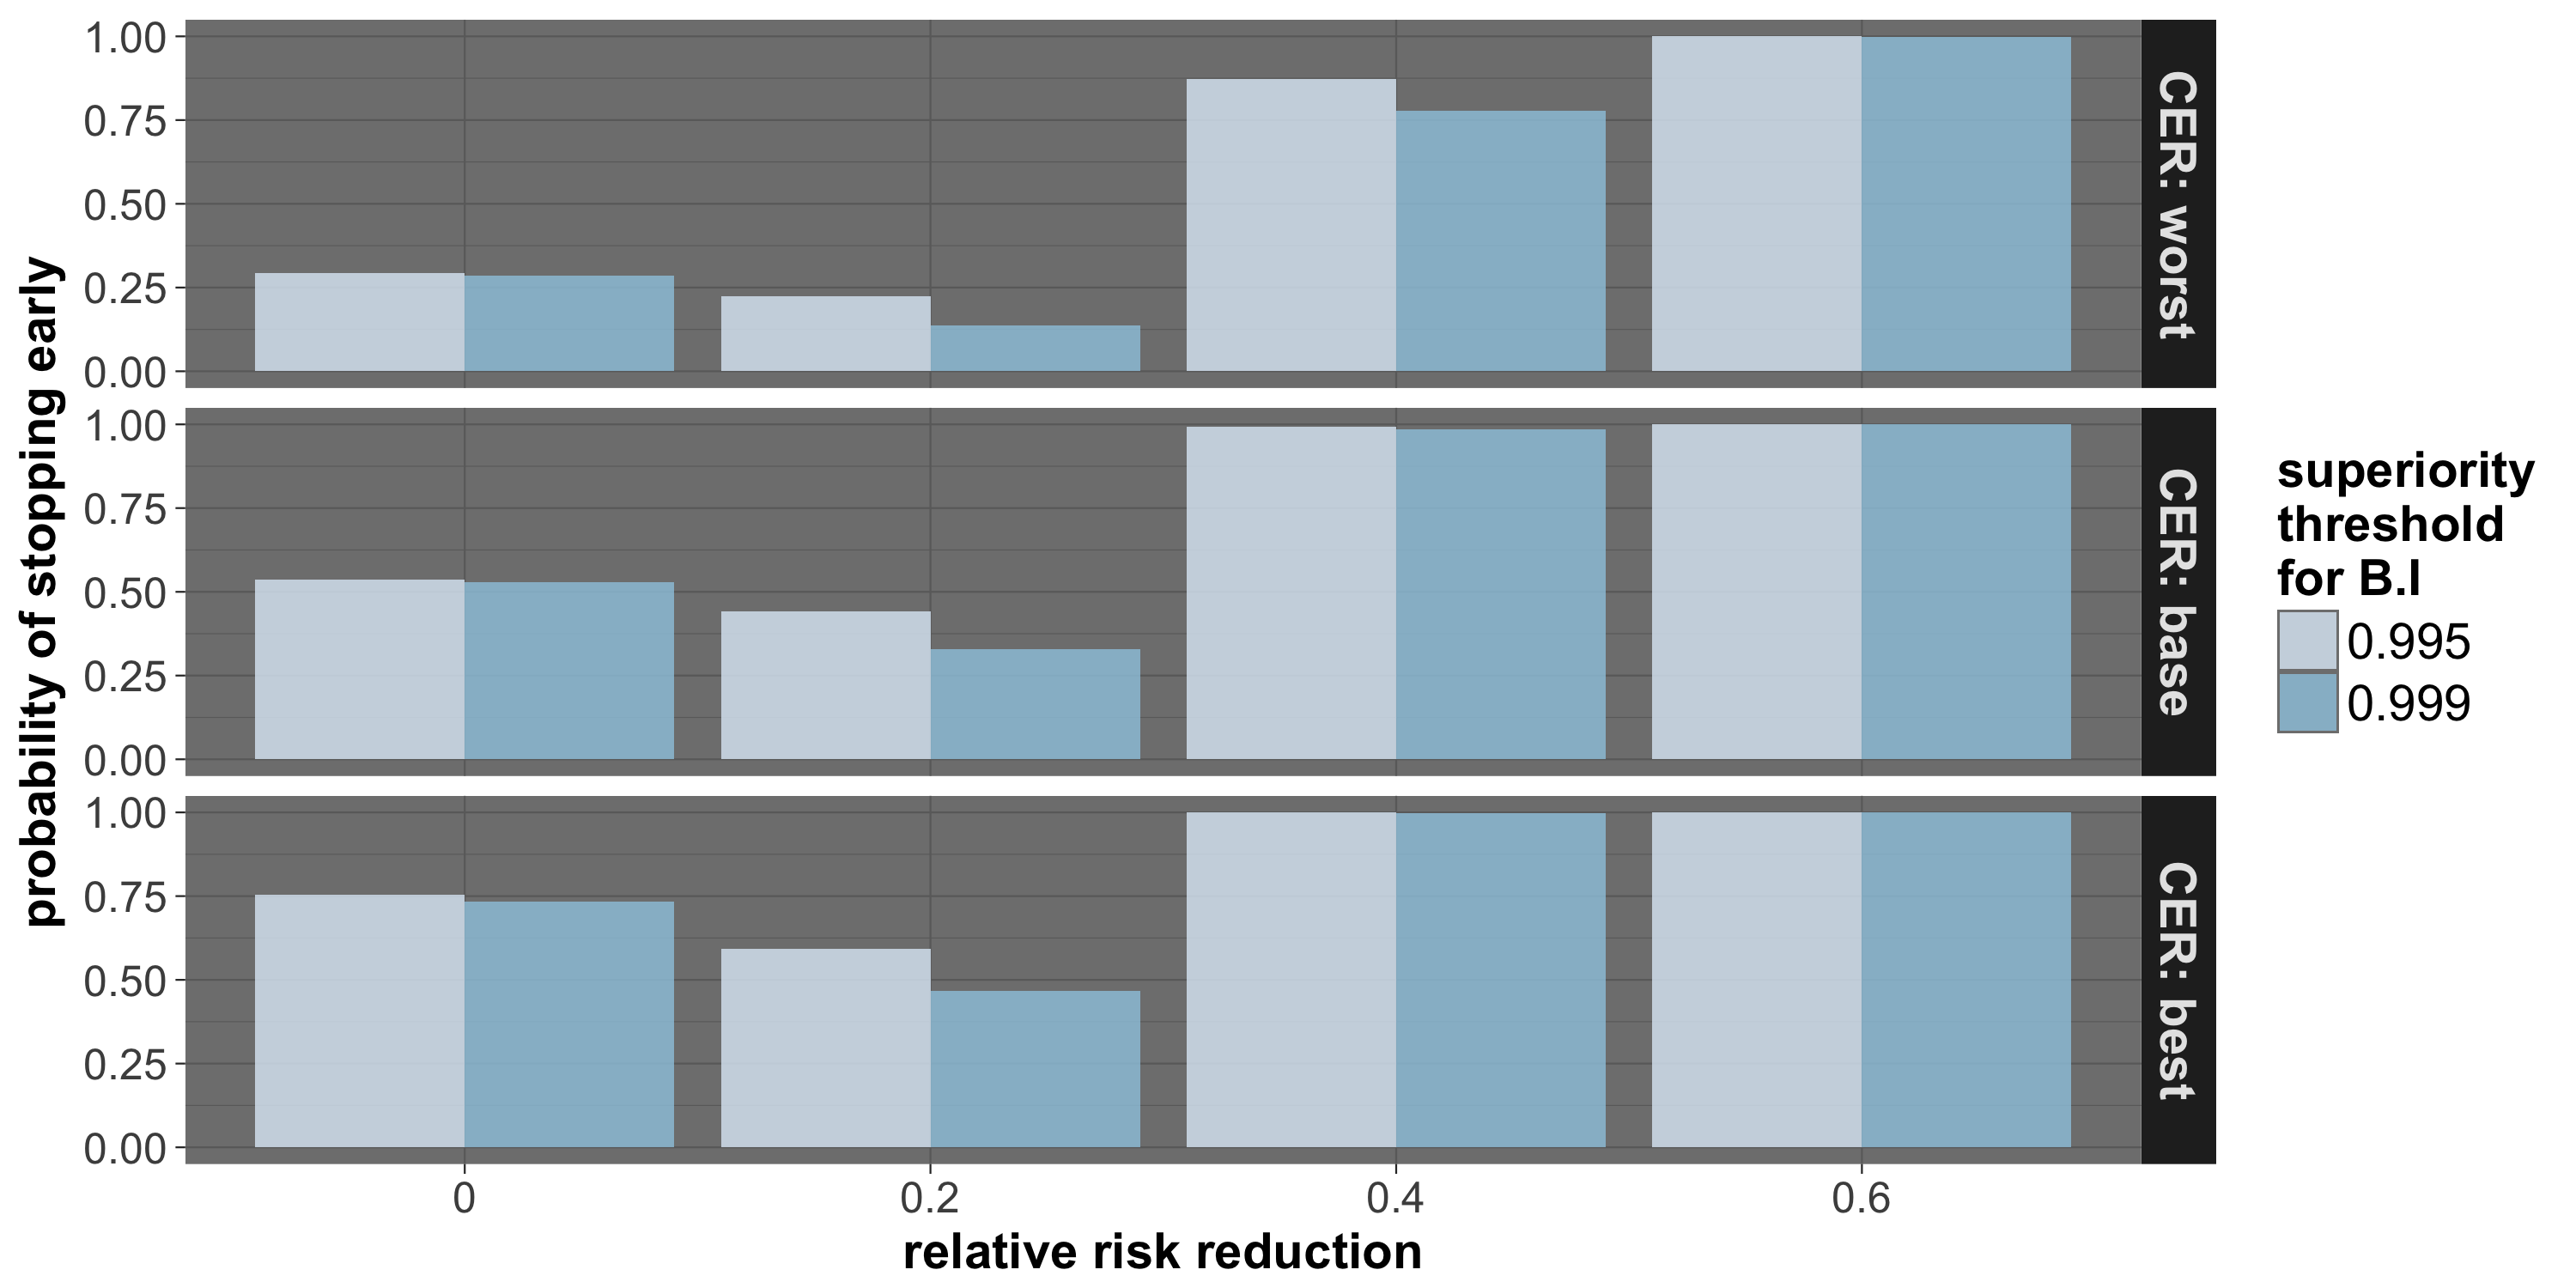
\includegraphics{../plots/3arm/early.png}
\end{figure}

Under the true RRR=0, there is a moderate to high chance of stopping for
futility for B.I. or L.P. (the chance increases as the CER improves).
There is negligible chance under all other scenarios. For B.I., there is
a high chance of stopping for superiority for true RRR=40\% and 60\% and
under all CER scenarios. There is negligible chance of stopping for
superiority for RRR=0\%, but a small to moderate chance (25-50\%) under
RRR=20\%. Stopping for L.P. follows a similar trend for stopping for
futility but shows a slight improvement over B.I. in stopping for
superiority under the true RRR=20\%.

\begin{figure}
\centering
  \caption{Probability of stopping (a) B.I. or (b) L.P. due to futility.  Stopping probabilities are presented for the
  three control event rates (CER – rows), four relative risk reductions (RRR – columns), and two superiority thresholds for B.I. (legend). Note that the legend and x axis labels should reflect the description given above, not as labeled on the graphic.}
  \begin{subfigure}{0.8\textwidth}
    \centering
    \caption{}
    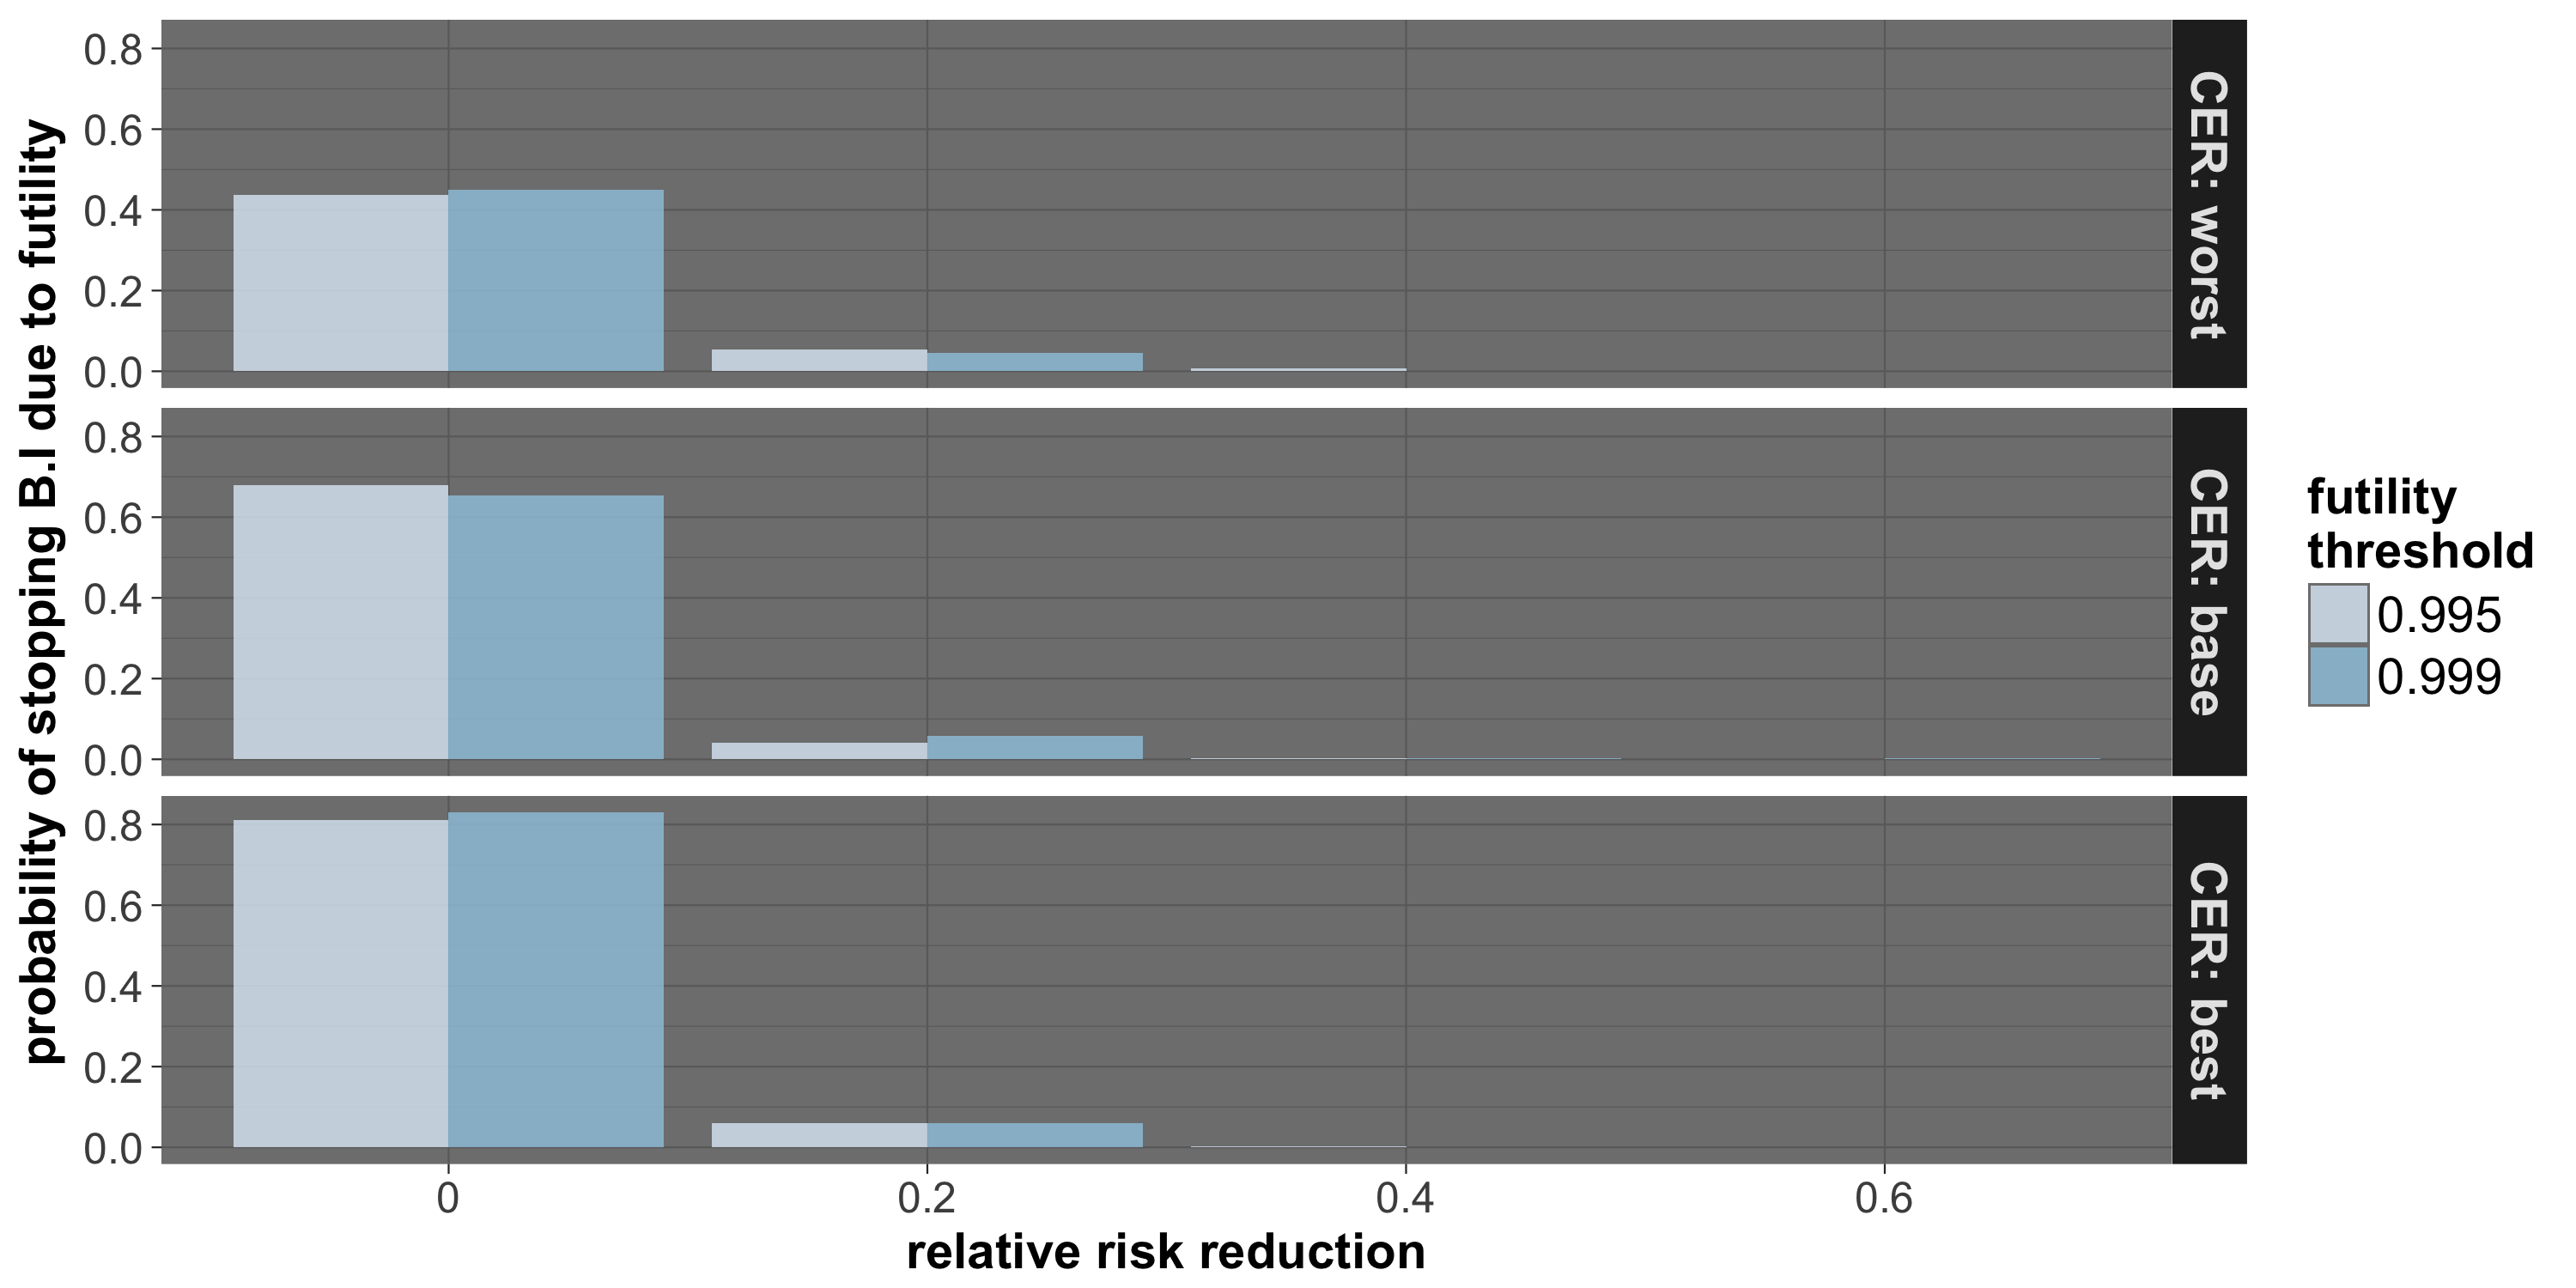
\includegraphics{../plots/3arm/futbi_3arm.png}
  \end{subfigure}
  \bigbreak
  \begin{subfigure}{0.8\textwidth}
    \centering
    \caption{}
    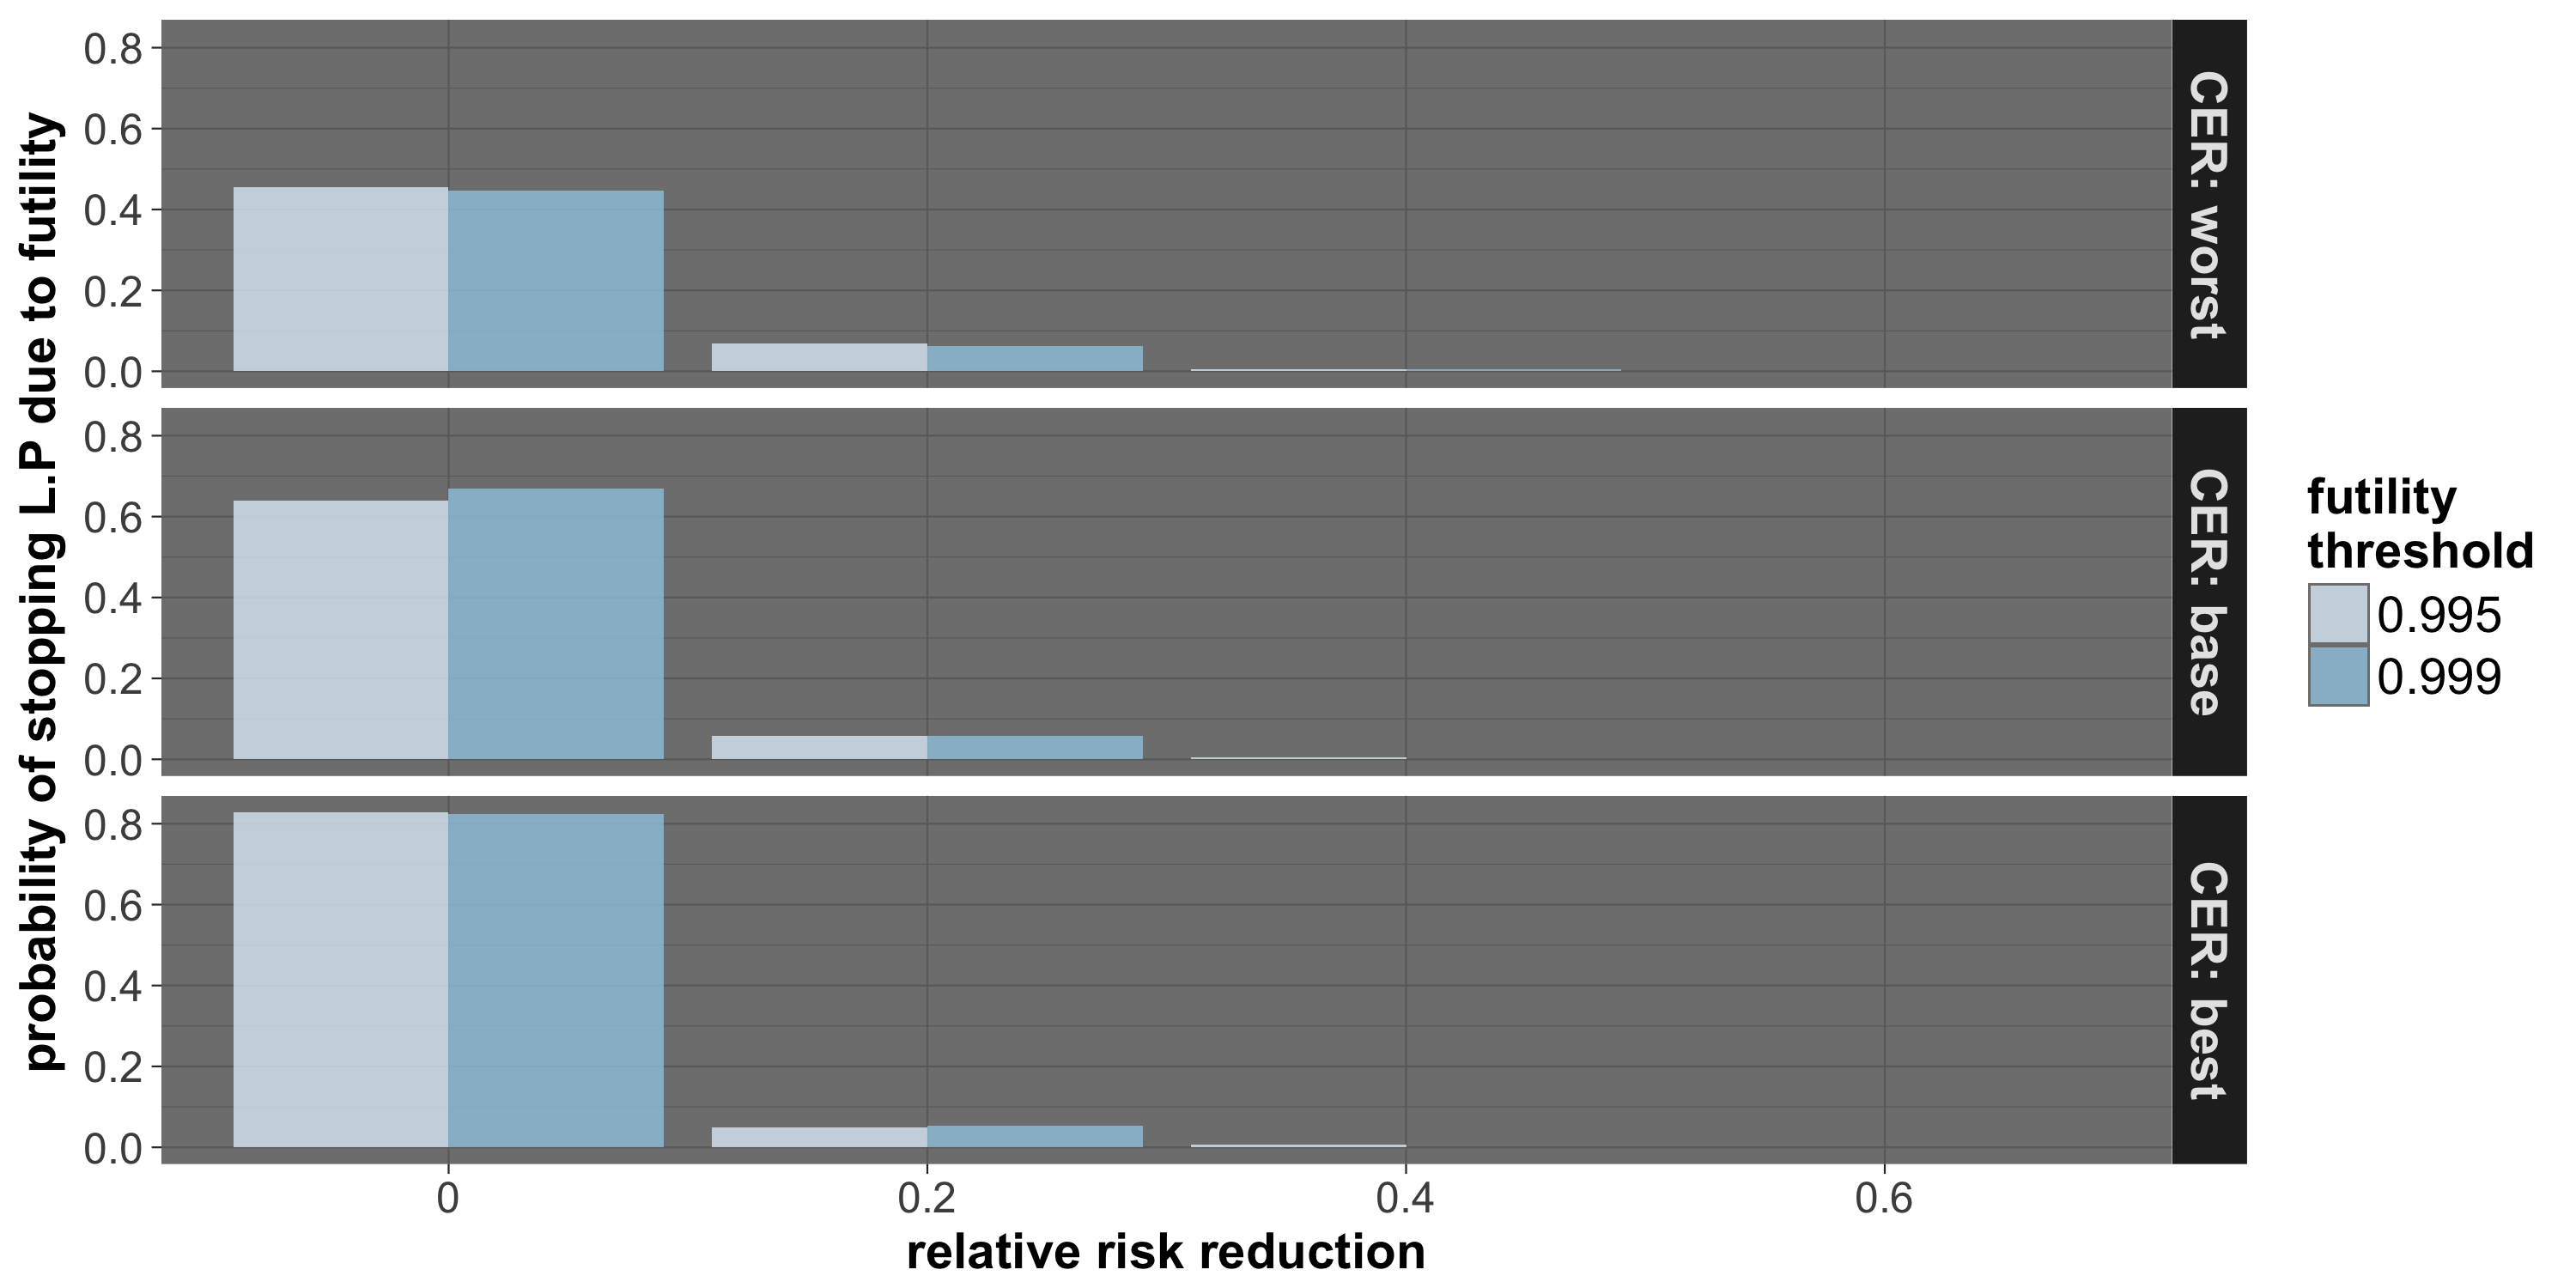
\includegraphics{../plots/3arm/futlp_3arm.png}
  \end{subfigure}
\end{figure}

\begin{figure}
\centering
  \caption{Probability of stopping (a) B.I. or (b) L.P. for superiority.  Stopping probabilities are presented for the
  three control event rates (CER – rows), four relative risk reductions (RRR – columns), and two superiority thresholds for B.I. (legend). Note that the legend and x axis labels should reflect the description given above, not as labeled on the graphic.}
  \begin{subfigure}{0.8\textwidth}
    \centering
    \caption{}
    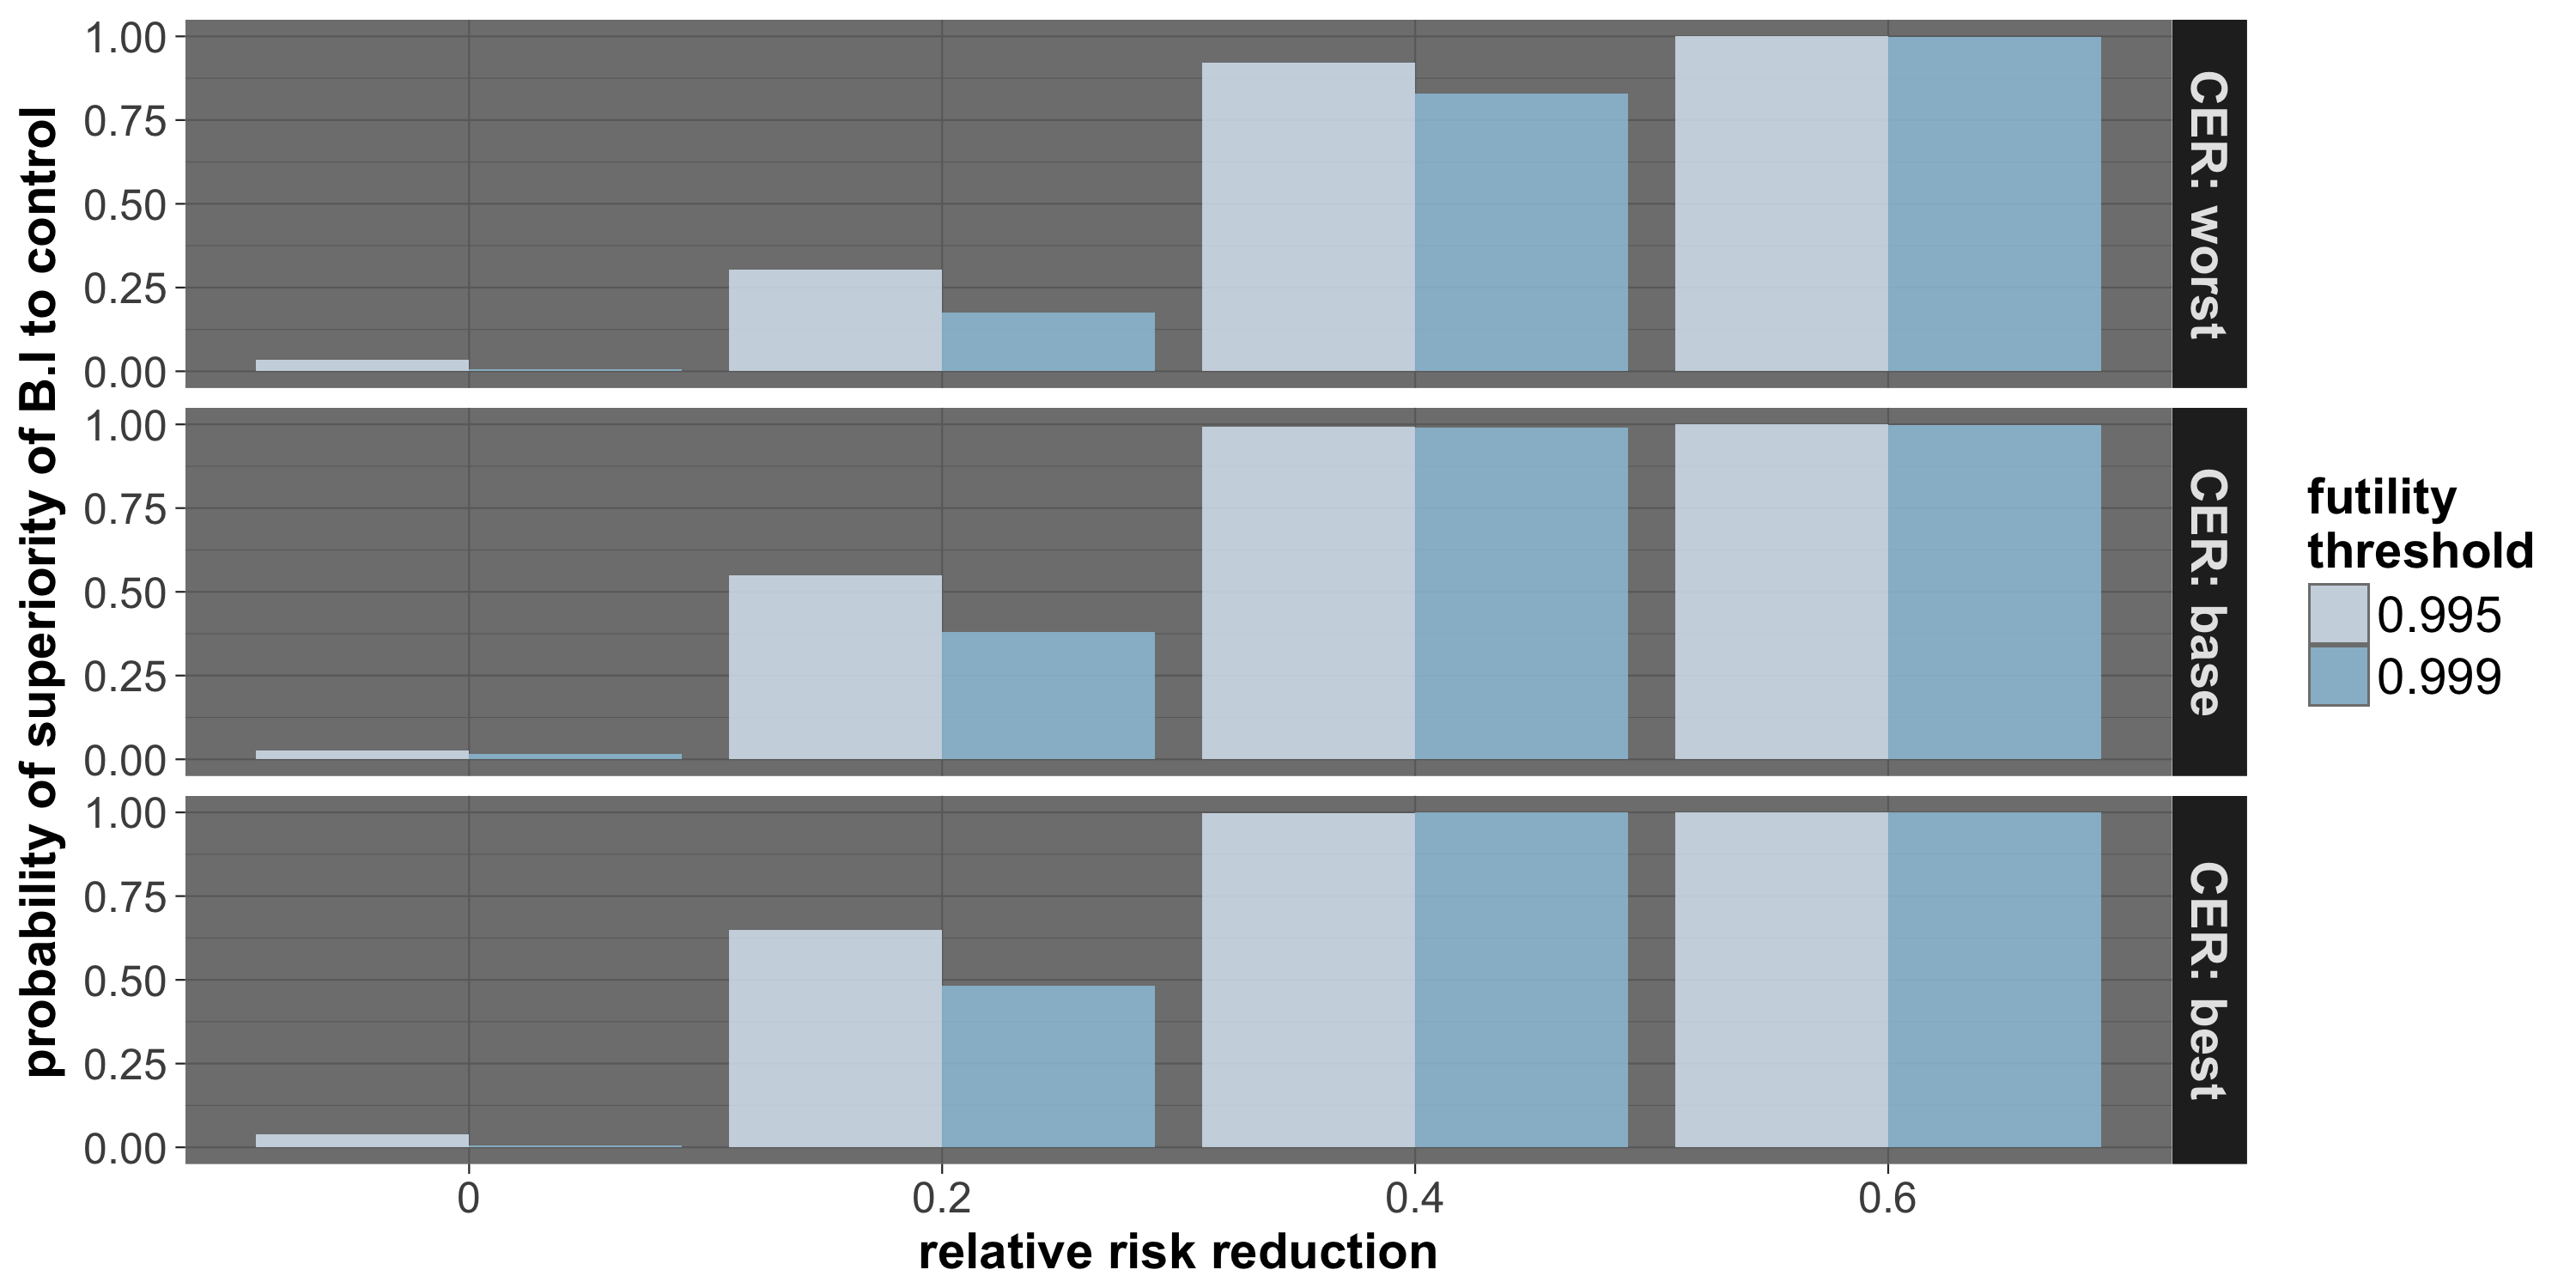
\includegraphics{../plots/3arm/supbi_3arm.png}
  \end{subfigure}
  \bigbreak
  \begin{subfigure}{0.8\textwidth}
    \centering
    \caption{}
    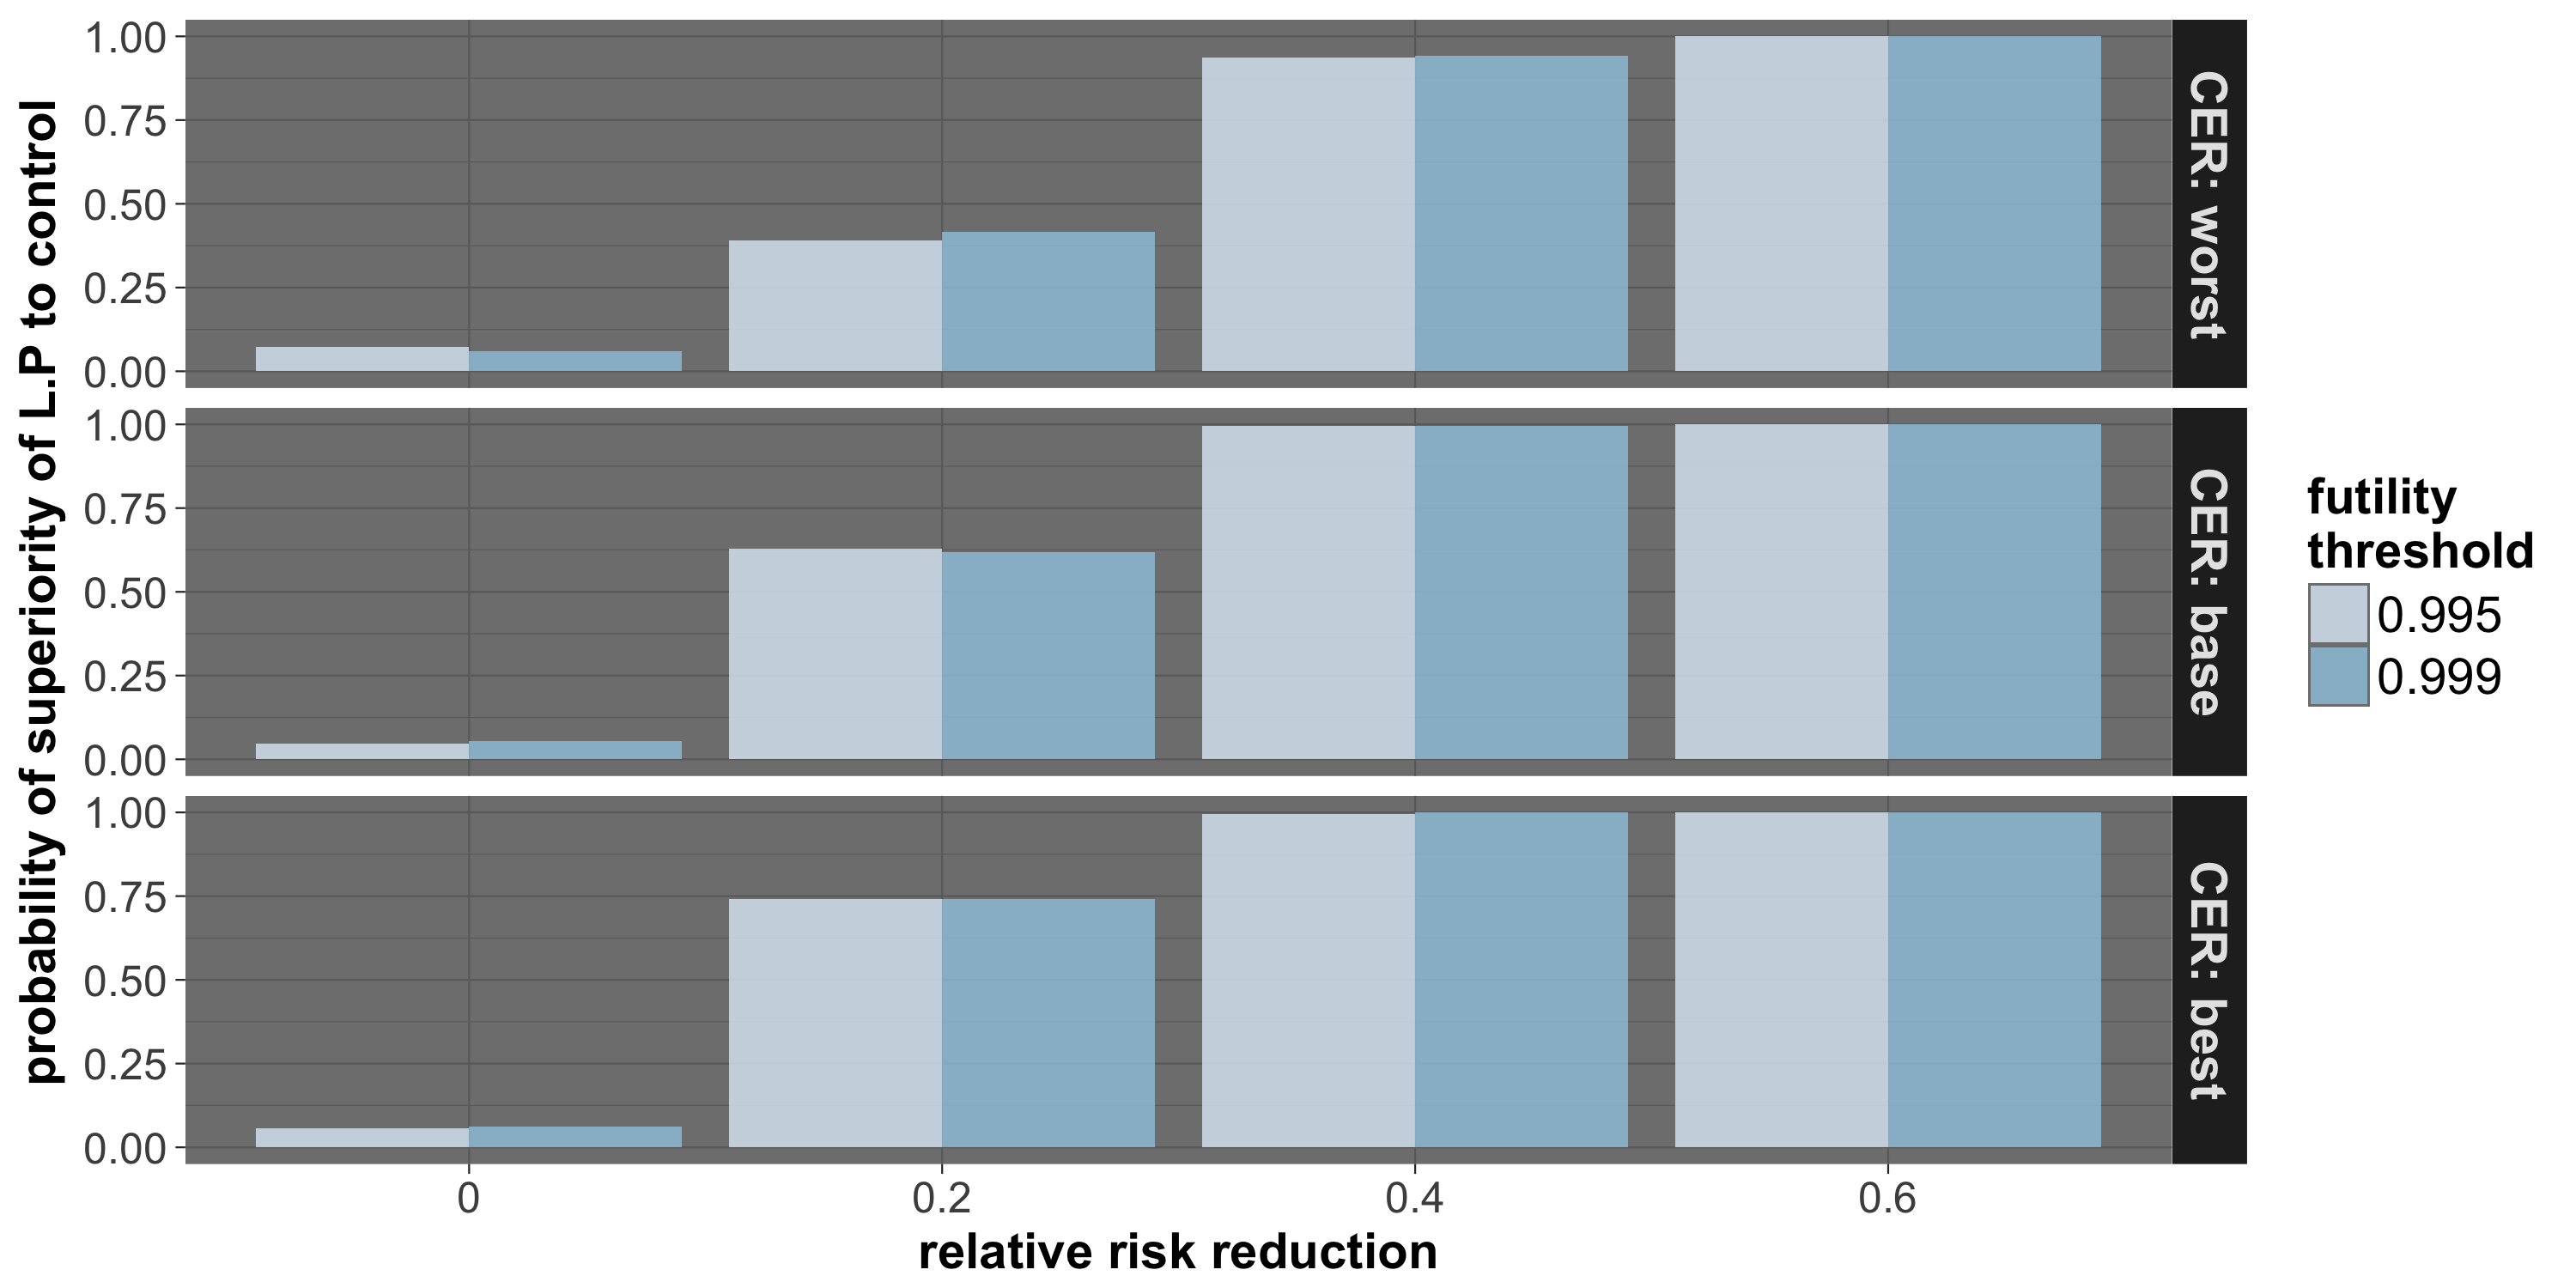
\includegraphics{../plots/3arm/suplp_3arm.png}
  \end{subfigure}
\end{figure}

\hypertarget{p-values-at-trial-termination-when-a-true-effect-exists-1}{%
\paragraph{P-values at trial termination when a true effect
exists}\label{p-values-at-trial-termination-when-a-true-effect-exists-1}}

Figure 17 presents the categorical distribution of p-values
(\textless{}5\%, 5-10\%, or \textgreater{}10\%) upon trial termination
(stopping early or reaching max. allowed sample size). Figure 18
presents the divide of p-values when stopping for futility ((a) B.I.,
(b) L.P.) and Figure 19 for and superiority ((a) B.I., (b) L.P.). The
overall probability of observing a p-value less than 5\% (i.e., a
conventionally statistically significant difference) is high or close to
100\% in scenarios when RRR=40\% or 60\% across all CER scenarios for
outcomes p1 and p2. Outcome s has a greater proportion of p-values being
\textgreater{}10\% in these scenarios. As the true RRR decreases, a
higher proportion of p-values are \textgreater{}10\% across all
scenarios and outcomes.

\begin{figure}
  \caption{Overall probability at trial termination that the p-value (from Fisher’s exact test) at termination of the
  trial is below 5\%, between 5\% and 10\% and greater than 10\%. The rows represent the three control even rate
  scenarios and the four columns present the four relative risk reduction scenarios.}
  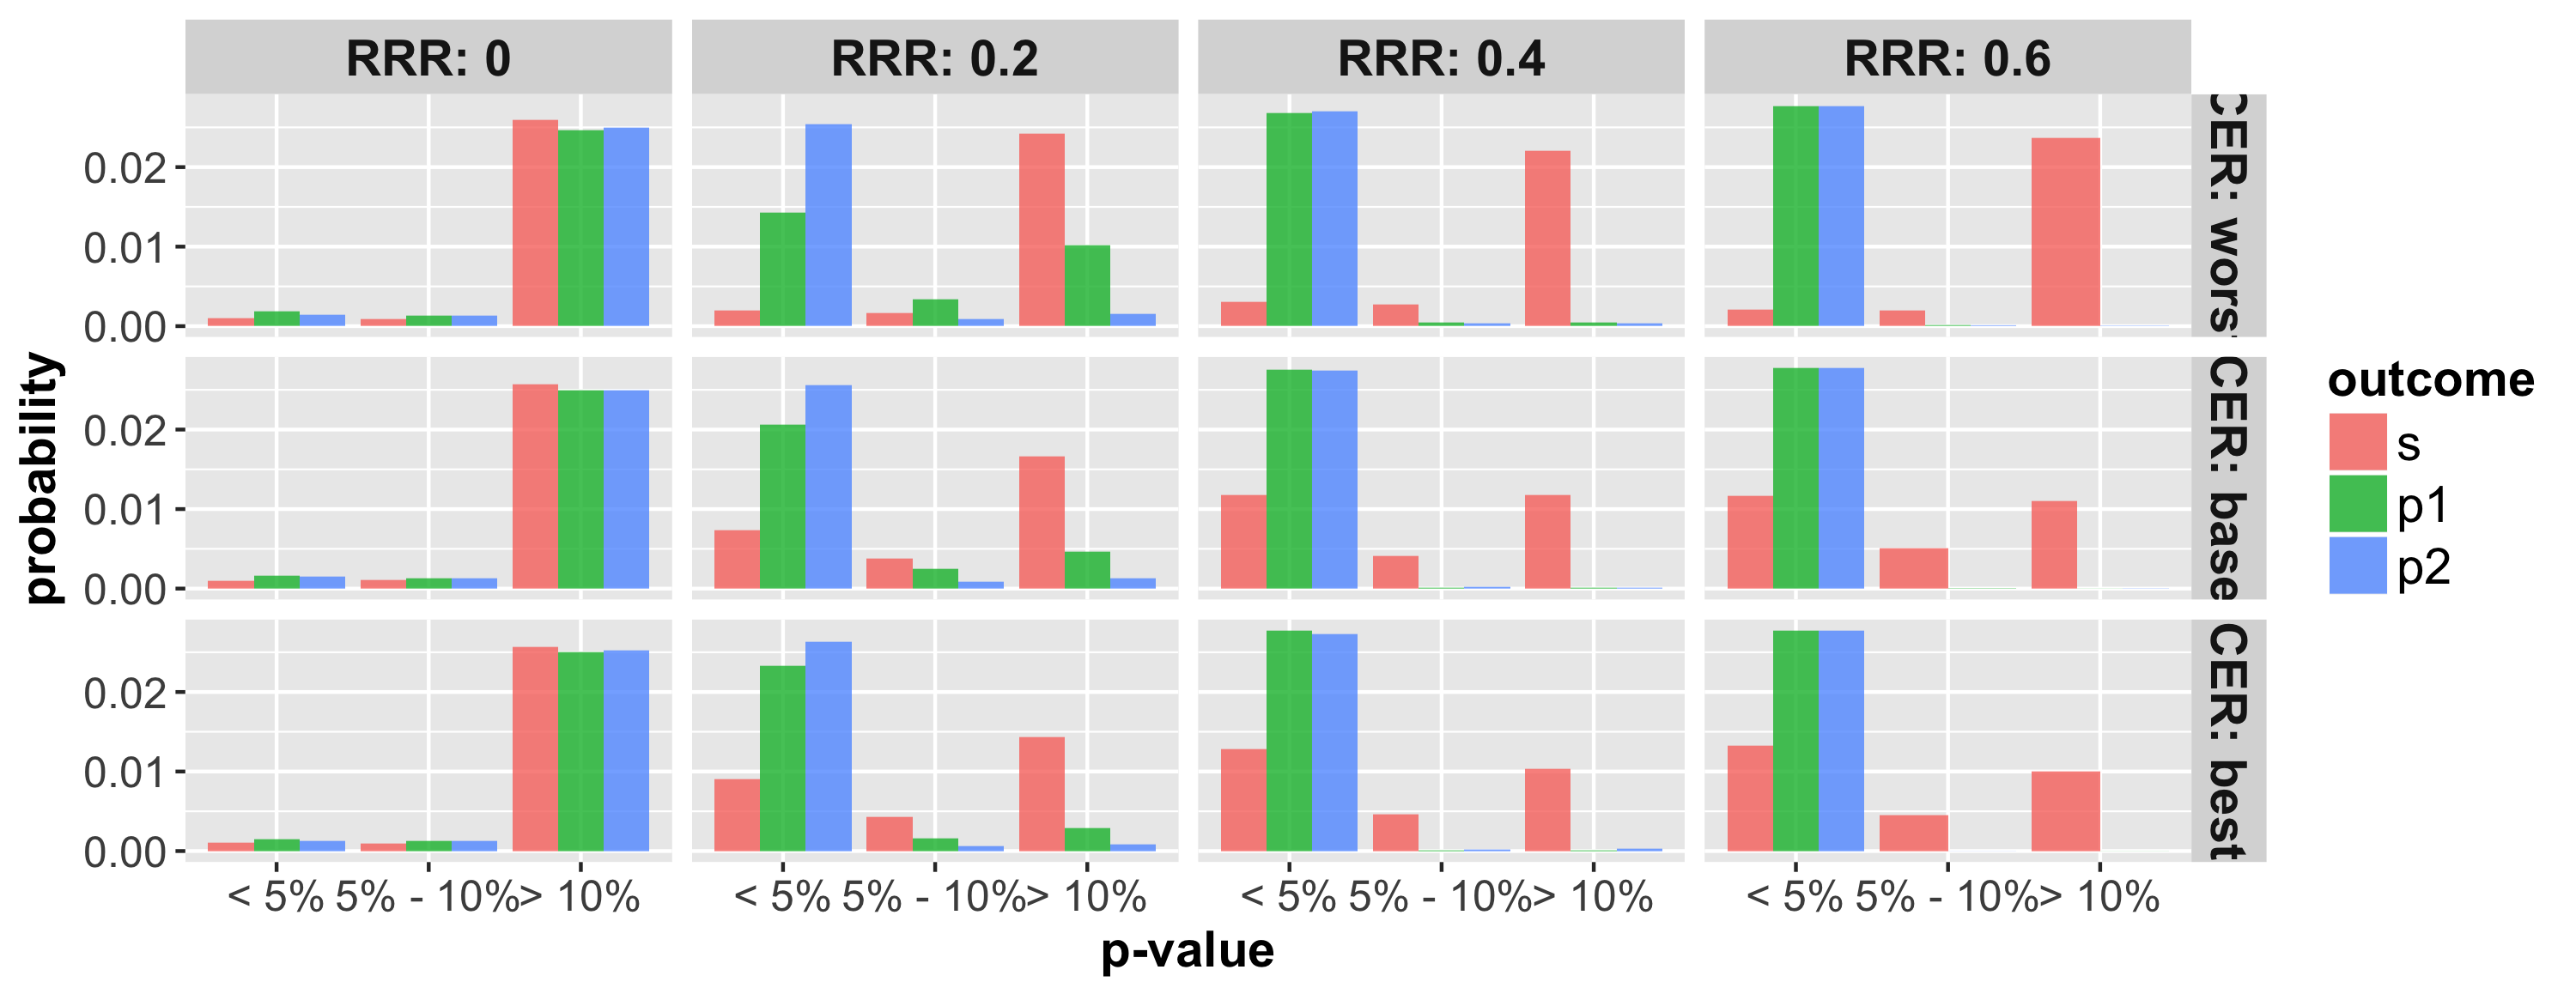
\includegraphics{../plots/3arm/p_value_3arm.png}
\end{figure}

In the situations where the trial is stopped early for futility (Figure
18) under the true RRR=0, the majority of p-values for all outcomes are
greater than 10\%. Reflecting that stopping for futility is less likely
under the other scenarios, only a small number of p-values are found for
these cases. When stopping for superiority (Figure 19) for both B.I. and
L.P., a high proportion of p-values for outcomes p1 and p2 are less than
5\% under true RRR=40\% and 60\%. A high proportion of p-values for
outcome s are greater than 10\% for all scenarios.

\begin{figure}
\centering
  \caption{Probability that the p-value (from Fisher’s exact test) at termination of the trial is below 5\%, between 5\%
  and 10\% and greater than 10\% for cases where trial was stopped for futility of (a) B.I or (b) L.P.  The rows
  represent the three control even rate scenarios and the four columns present four relative risk reduction scenarios.
  Note: In the figures below, the denominator in each figure is the number of simulations (not the number of trials
  stopped for futility or superiority, and thus, the proportions do not add up to 100\% within one figure. Further, the
  figures do not include simulations where the trial went to the maximum allowed sample size. The bars should be
  interpreted with respect to the relative proportion that fit in each category.}
  \begin{subfigure}{0.8\textwidth}
    \centering
    \caption{}
    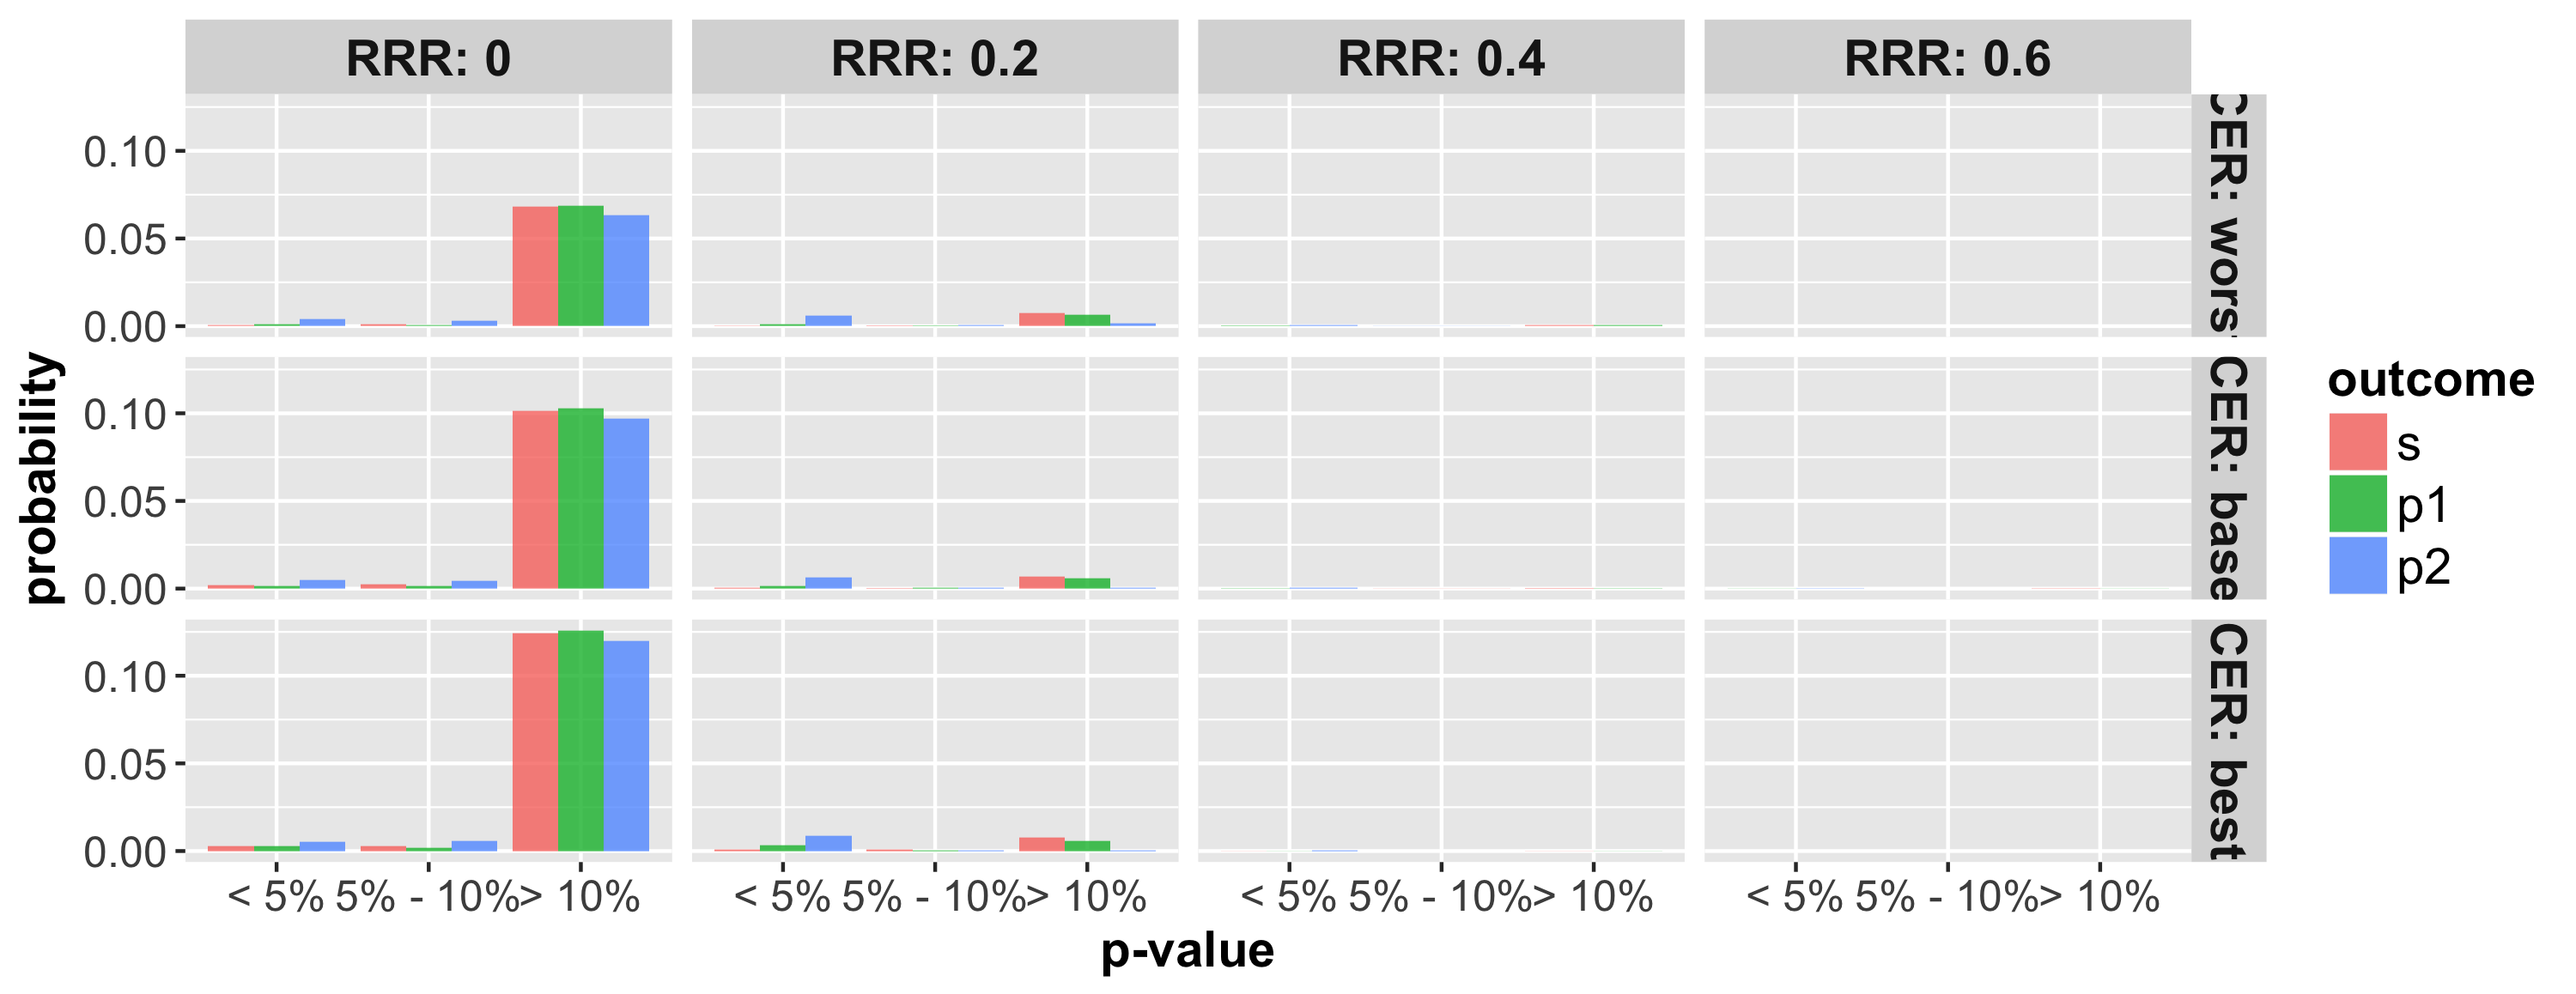
\includegraphics{../plots/3arm/p_value_futbi_3arm.png}
  \end{subfigure}
  \bigbreak
  \begin{subfigure}{0.8\textwidth}
    \centering
    \caption{}
    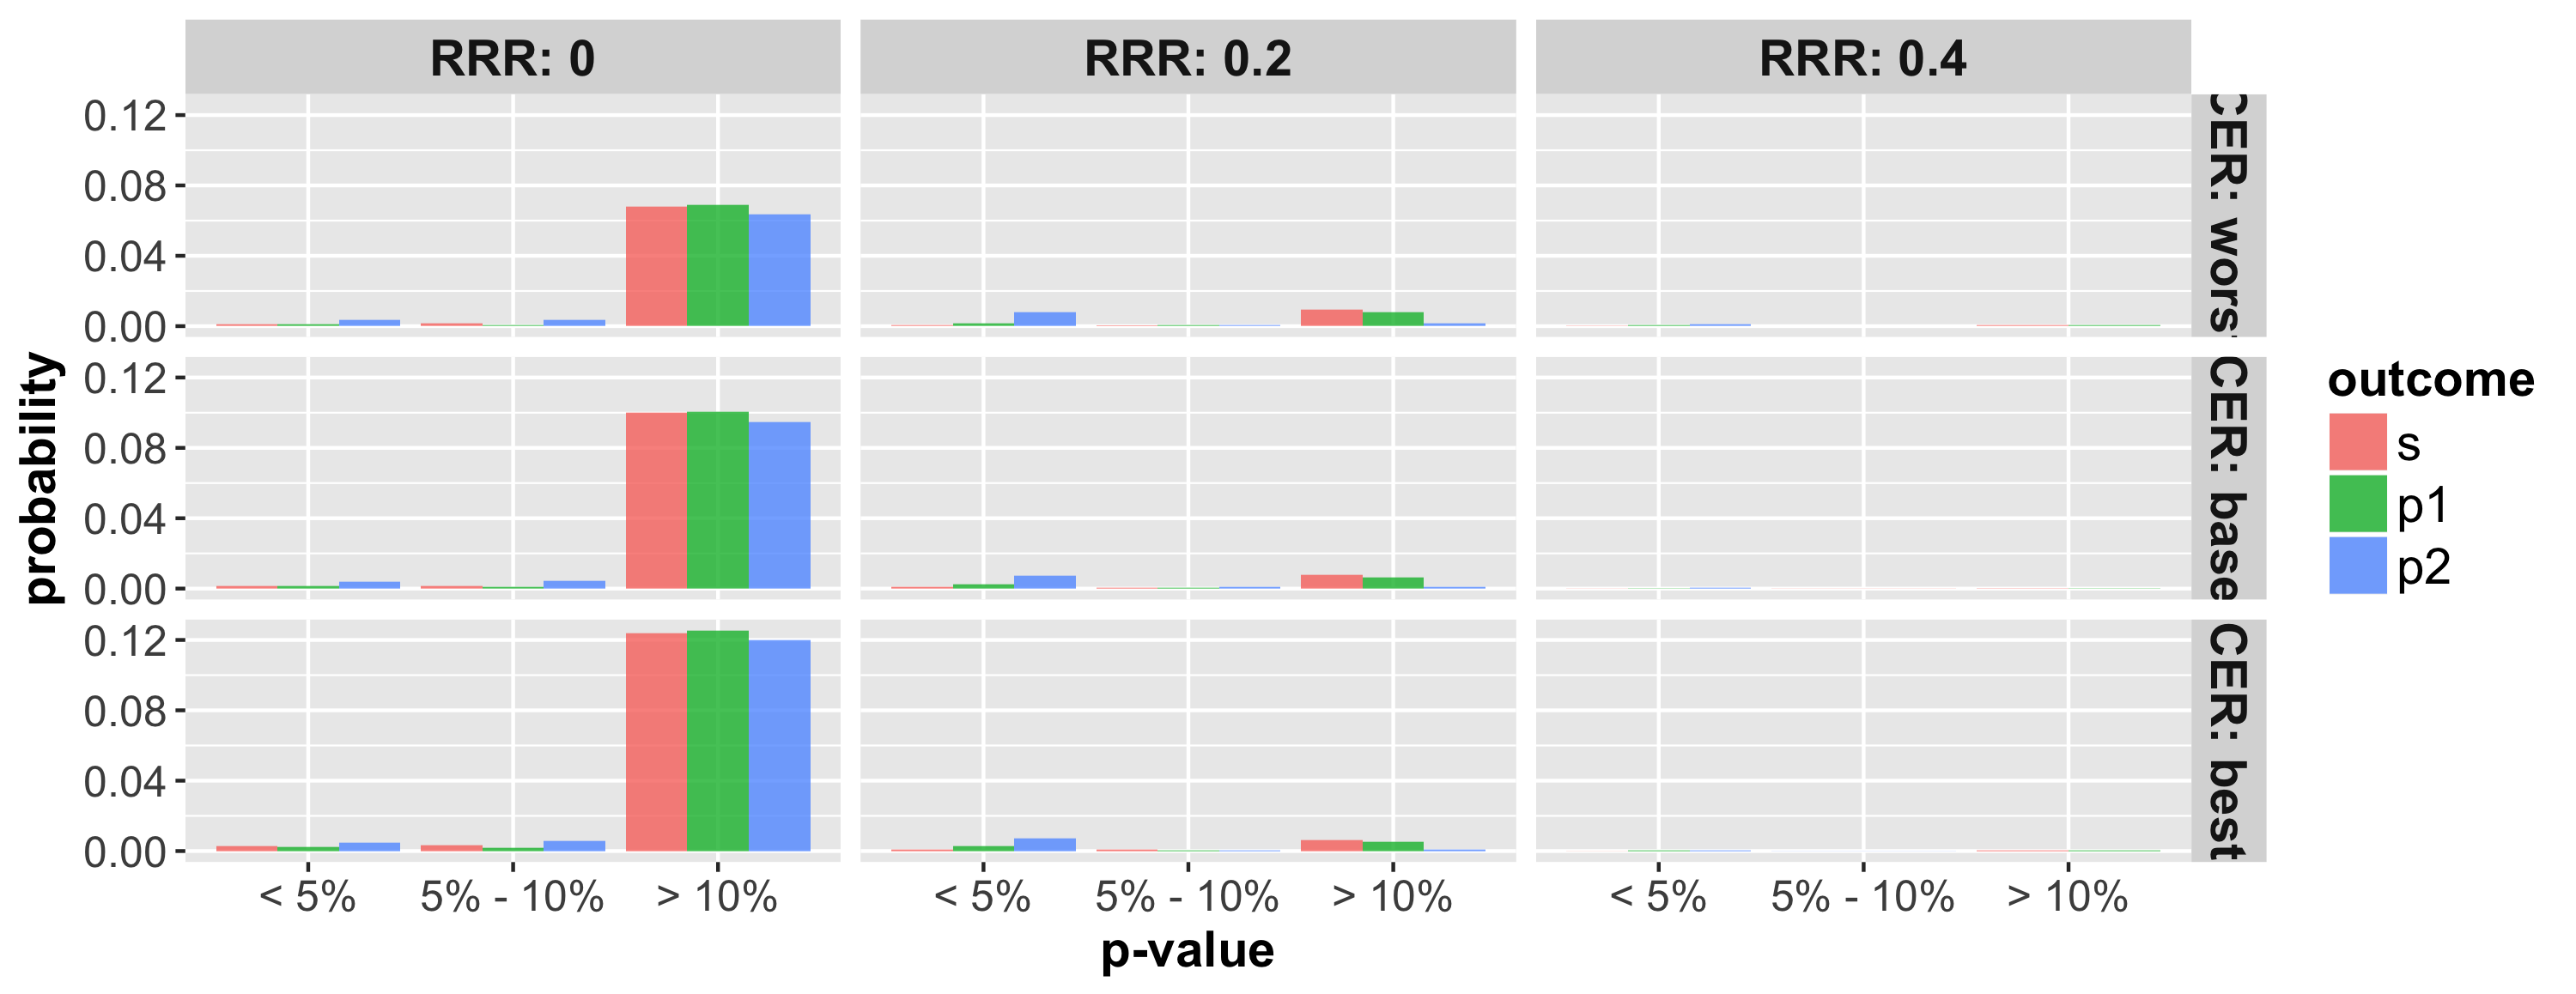
\includegraphics{../plots/3arm/p_value_futlp_3arm.png}
  \end{subfigure}
\end{figure}

\begin{figure}
\centering
  \caption{Probability that the p-value (from Fisher’s exact test) at termination of the trial is below 5\%, between 5\%
  and 10\% and greater than 10\% for cases where trial was stopped for superiority of (a) B.I or (b) L.P. The rows
  represent the three control even rate scenarios and the four columns present four relative risk reduction scenarios.
  Note: In the figures below, the denominator in each figure is the number of simulations (not the number of trials
  stopped for futility or superiority, and thus, the proportions do not add up to 100% within one figure. Further, the
  figures do not include simulations where the trial went to the maximum allowed sample size. The bars should be
  interpreted with respect to the relative proportion that fit in each category.}
  \begin{subfigure}{0.8\textwidth}
    \centering
    \caption{}
    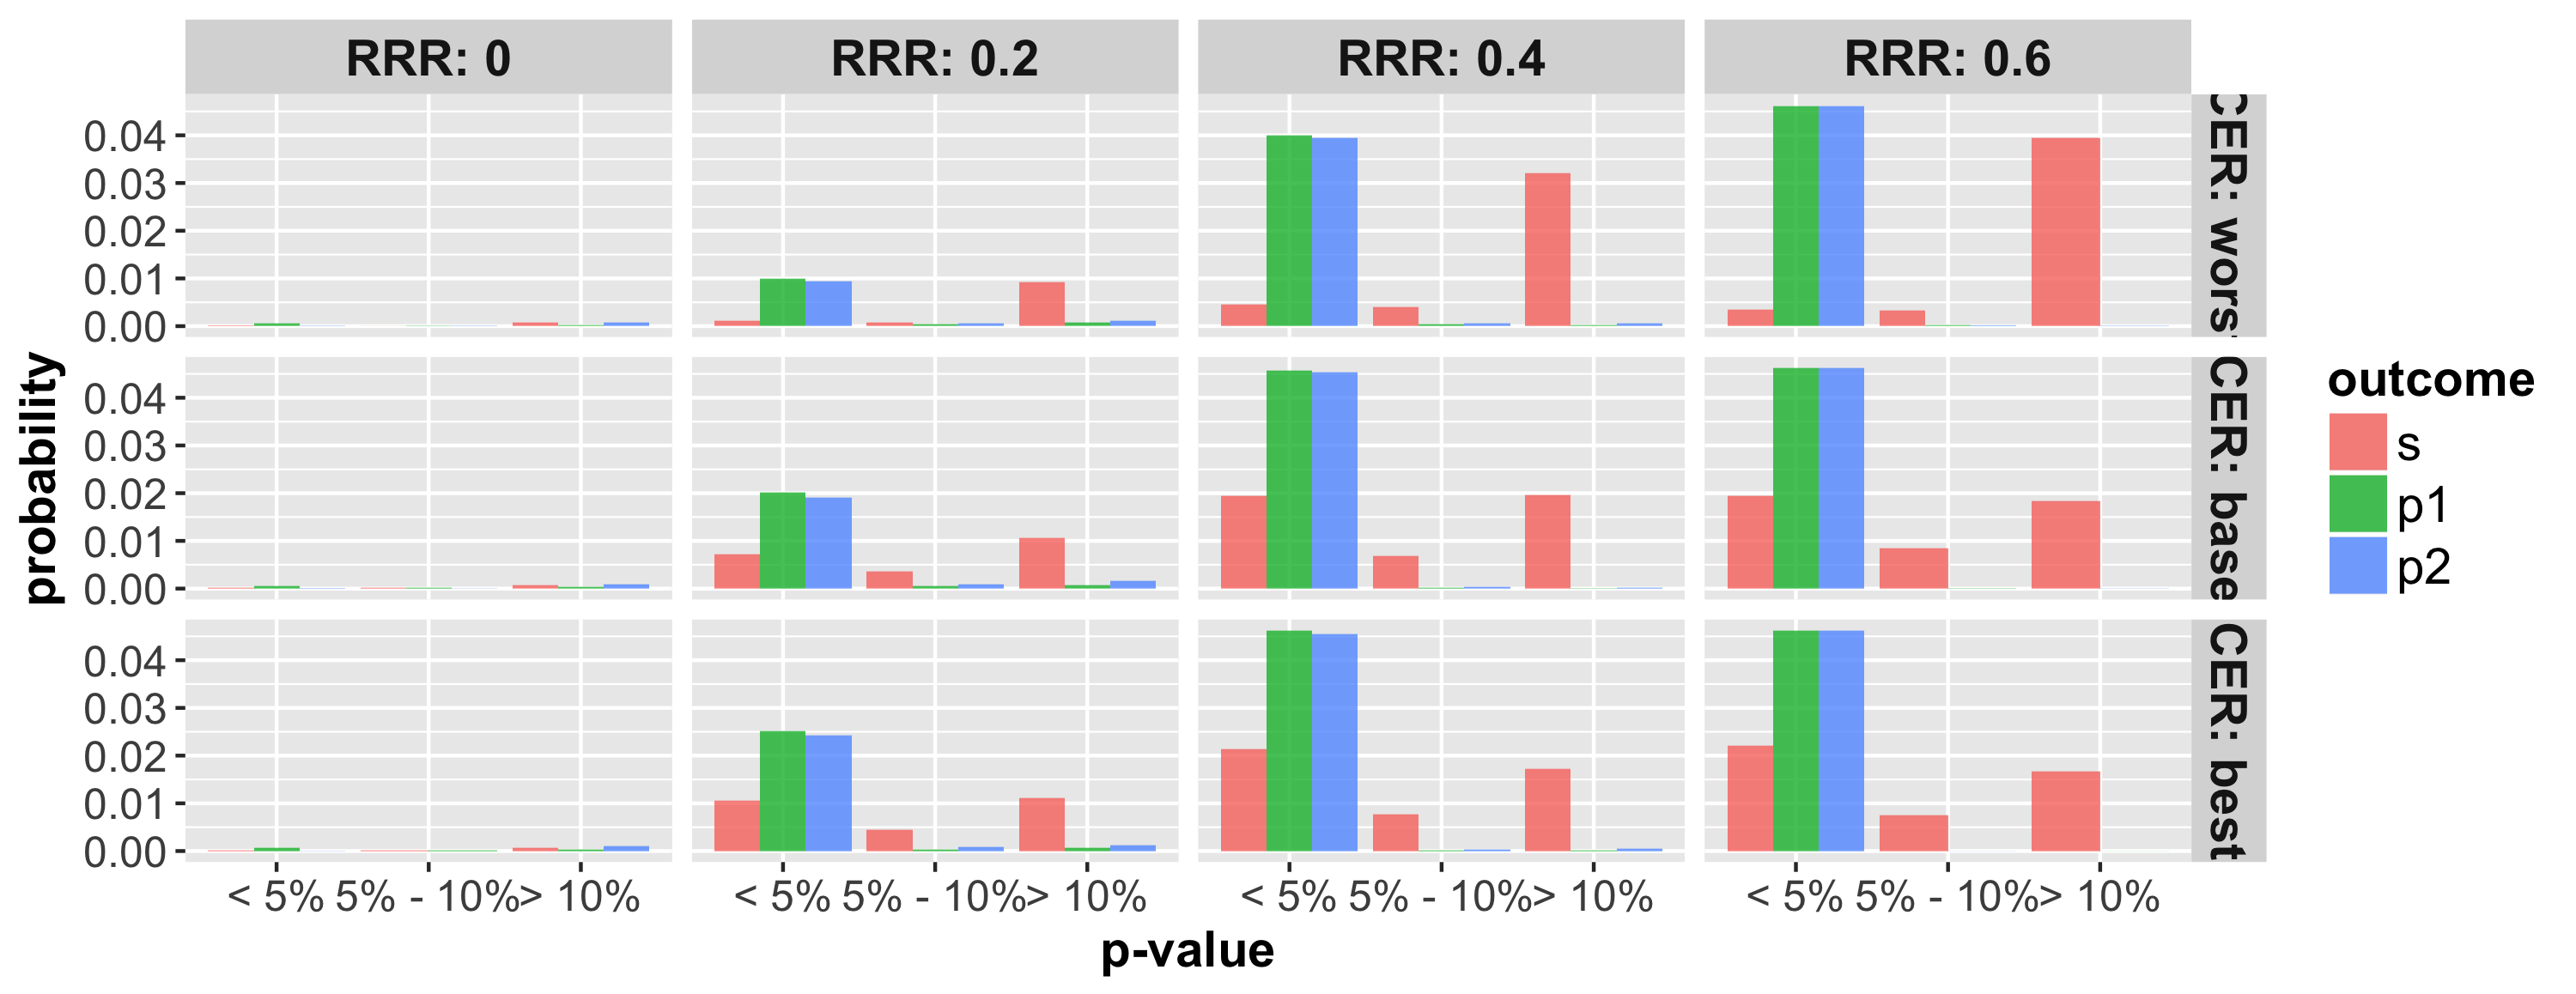
\includegraphics{../plots/3arm/p_value_supbi_3arm.png}
  \end{subfigure}
  \bigbreak
  \begin{subfigure}{0.8\textwidth}
    \centering
    \caption{}
    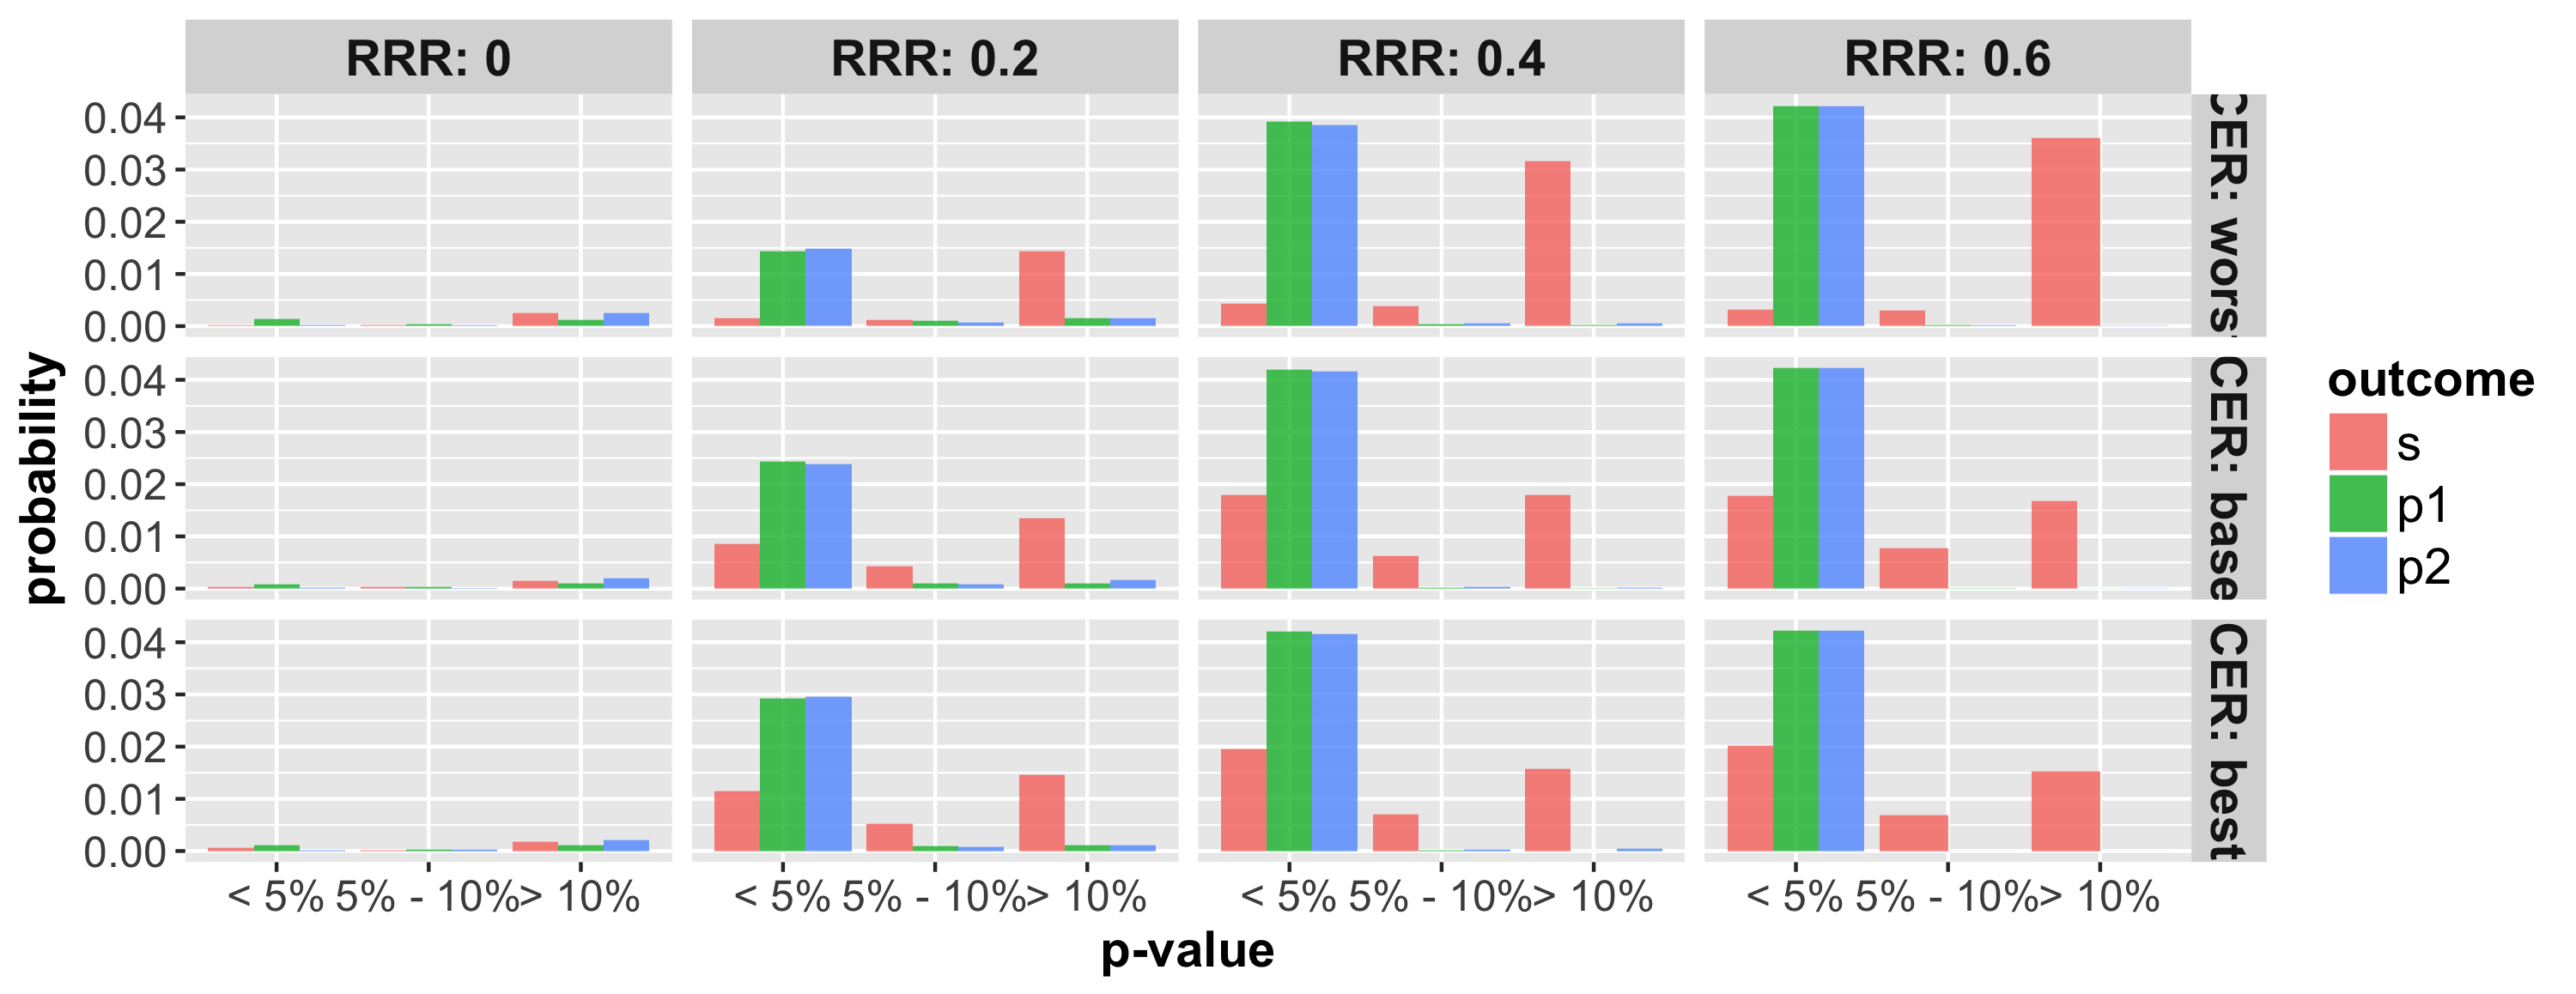
\includegraphics{../plots/3arm/p_value_suplp_3arm.png}
  \end{subfigure}
\end{figure}

\hypertarget{relative-risk-reduction-estimates-at-trial-termination-1}{%
\paragraph{Relative risk reduction estimates at trial
termination}\label{relative-risk-reduction-estimates-at-trial-termination-1}}

Figure 20 presents the distribution of relative risk reduction estimates
upon trial termination. Figure 21 ((a) B.I., (b) L.P.) and Figure 22
((a) B.I., (b) L.P.) present the distribution of relative risk reduction
estimates from trials stopped early for futility and superiority,
respectively. In general, the estimates of p1 and p2 exhibit much larger
precision.

\begin{figure}
  \caption{Distribution of relative risk reduction estimates (smoothed by a kernel density estimator) for the three
  control event rates (CER – rows), four relative risk reductions (RRR – columns) and the three outcomes (legend).}
  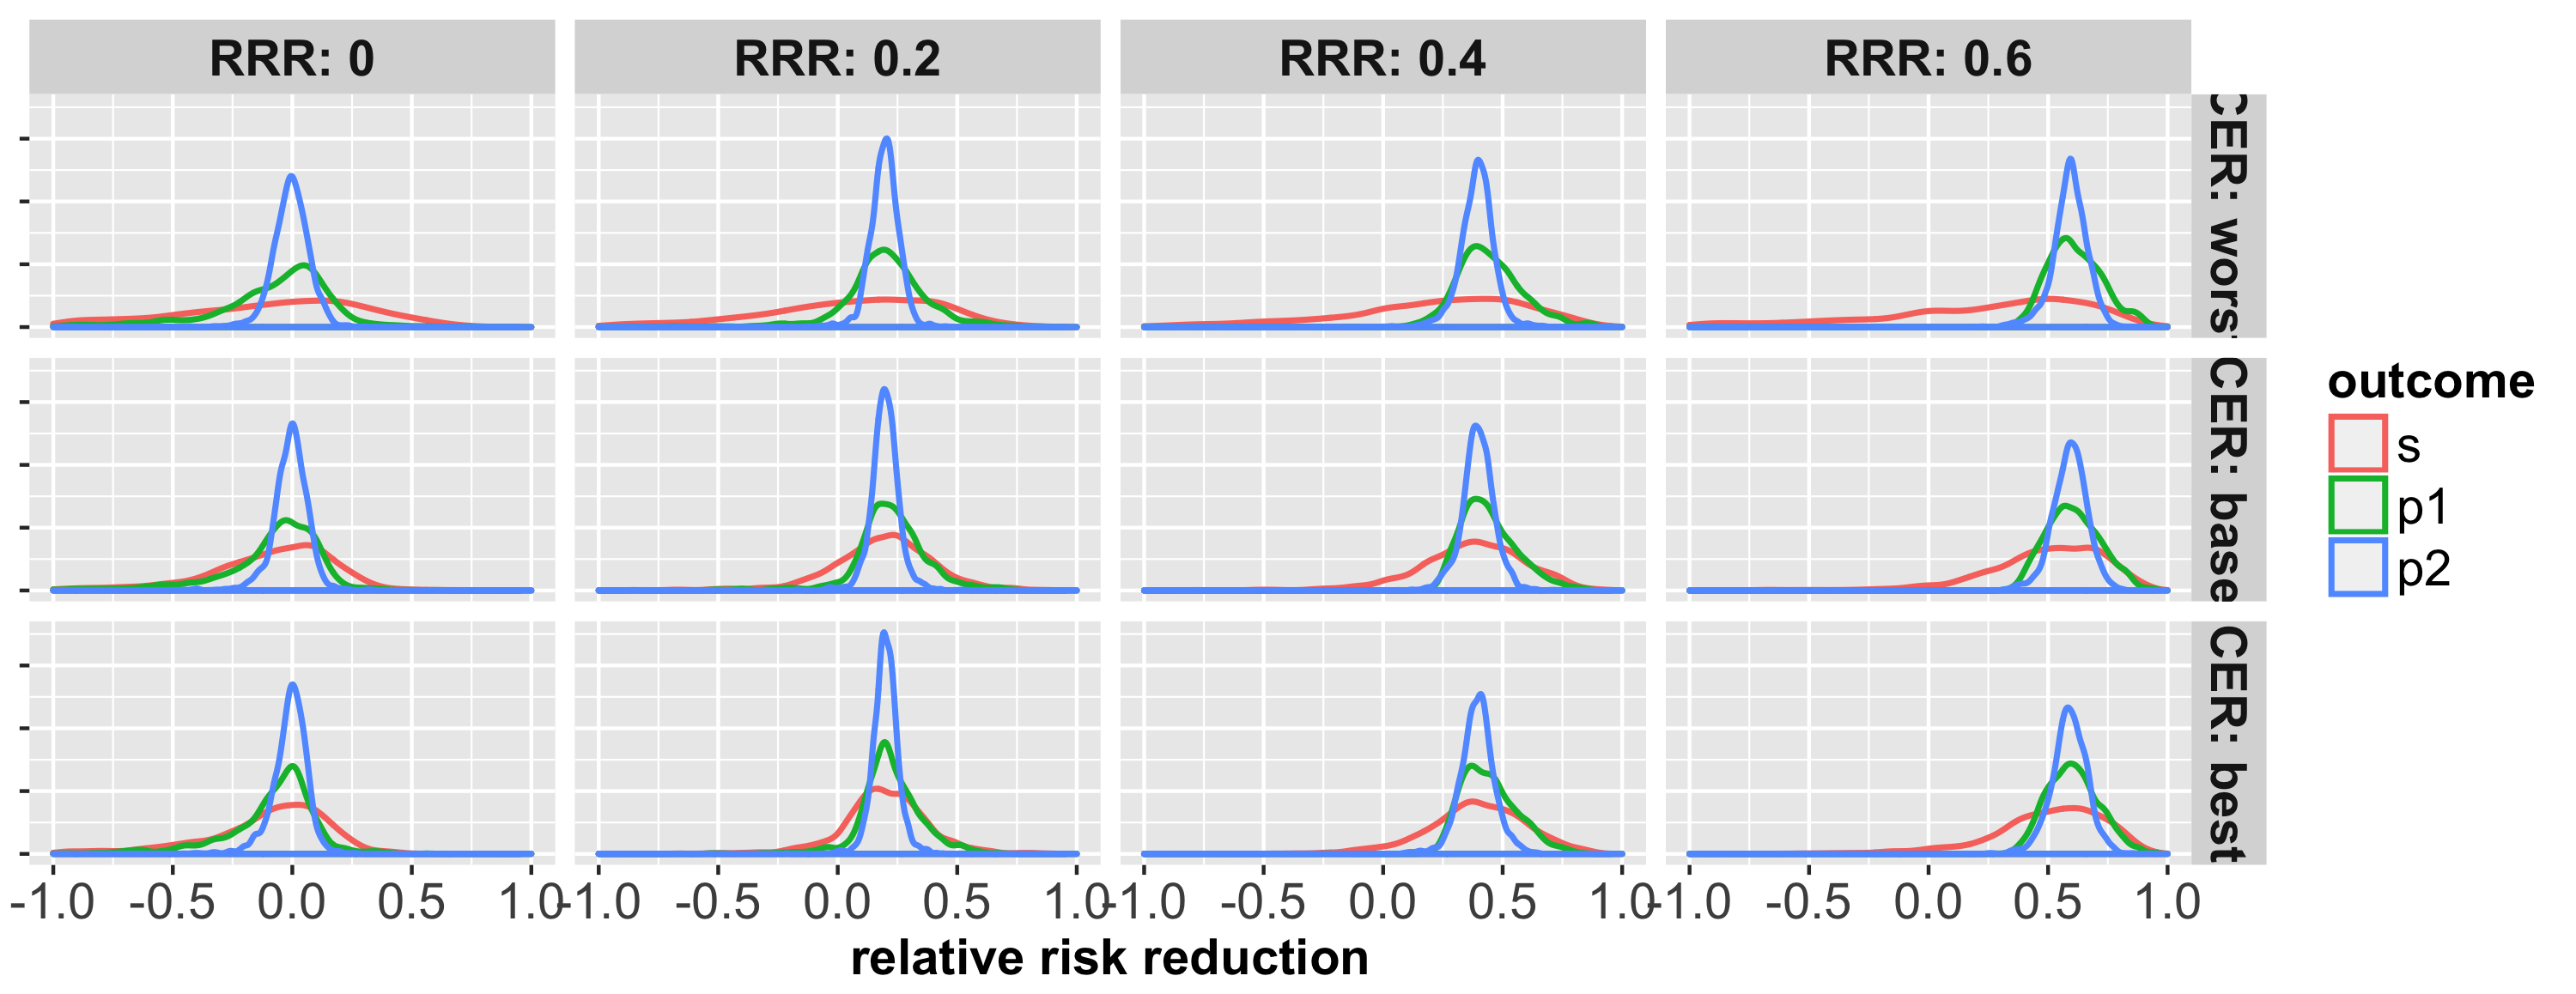
\includegraphics{../plots/3arm/RRRhat_3arm.png}
\end{figure}

When stopping for futility (Figure 21), outcome p2 is generally precise
and shows little bias. Outcomes p1 and s exhibit either small downward
bias for lower RRR or become overly diffuse for higher RRR. When
stopping for superiority, outcome p2 show little evidence of bias and
has good precision across all scenarios. Outcomes p1 and s have small
upward bias for lower RRR and show improvement in precision for higher
RRR.

\begin{figure}
\centering
  \caption{Distribution of relative risk reduction estimates after stopping early for futility of (a) B.I. or (b) L.P.
  Results are presented for the three control event rates by rows, four relative risk reductions (by columns) and the
  three outcomes (legend).}
  \begin{subfigure}{0.8\textwidth}
    \centering
    \caption{}
    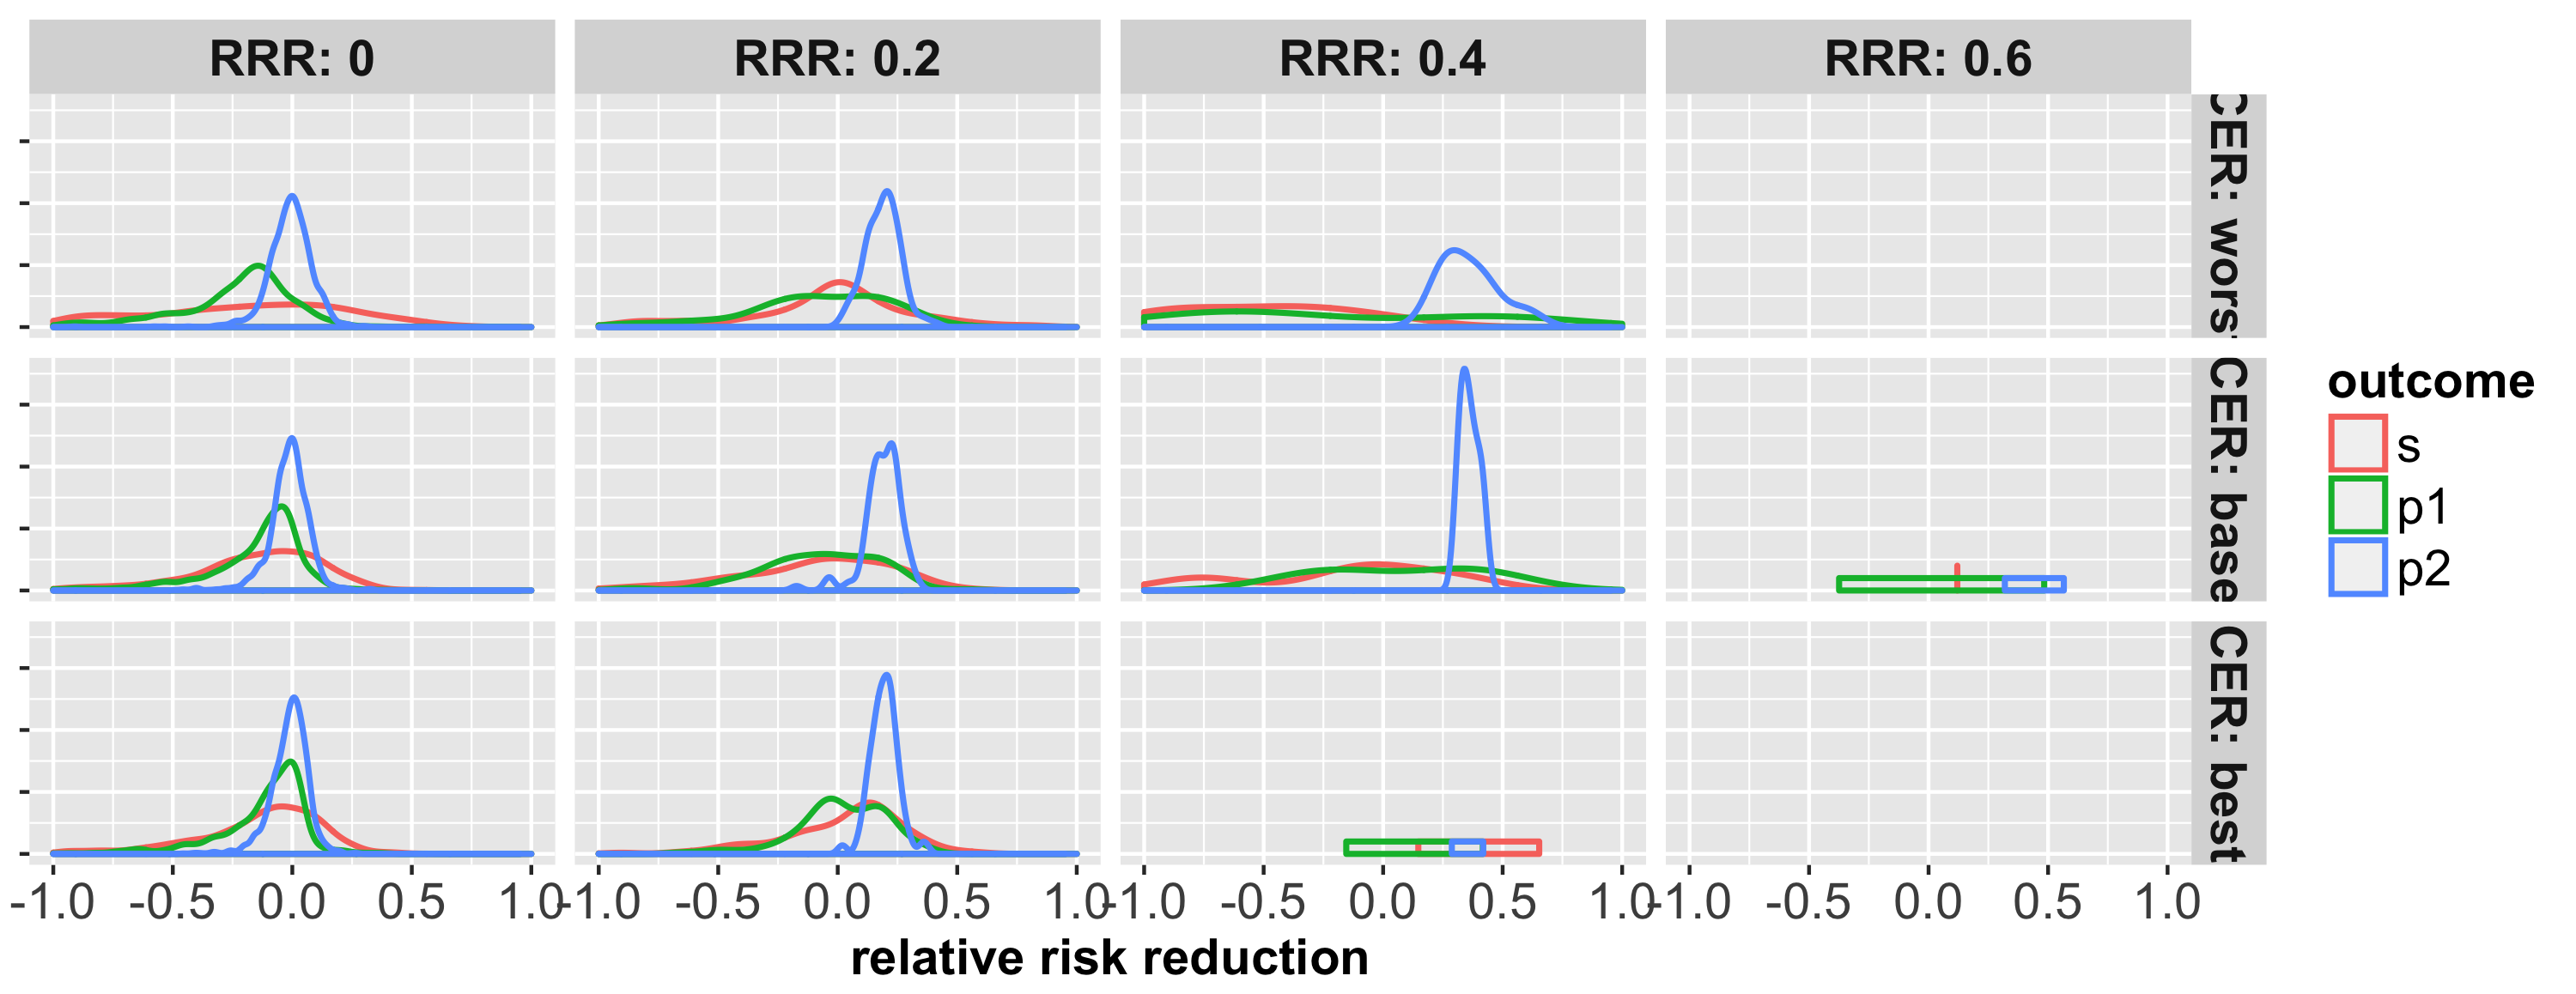
\includegraphics{../plots/3arm/RRRhat_futbi_3arm.png}
  \end{subfigure}
  \bigbreak
  \begin{subfigure}{0.8\textwidth}
    \centering
    \caption{}
    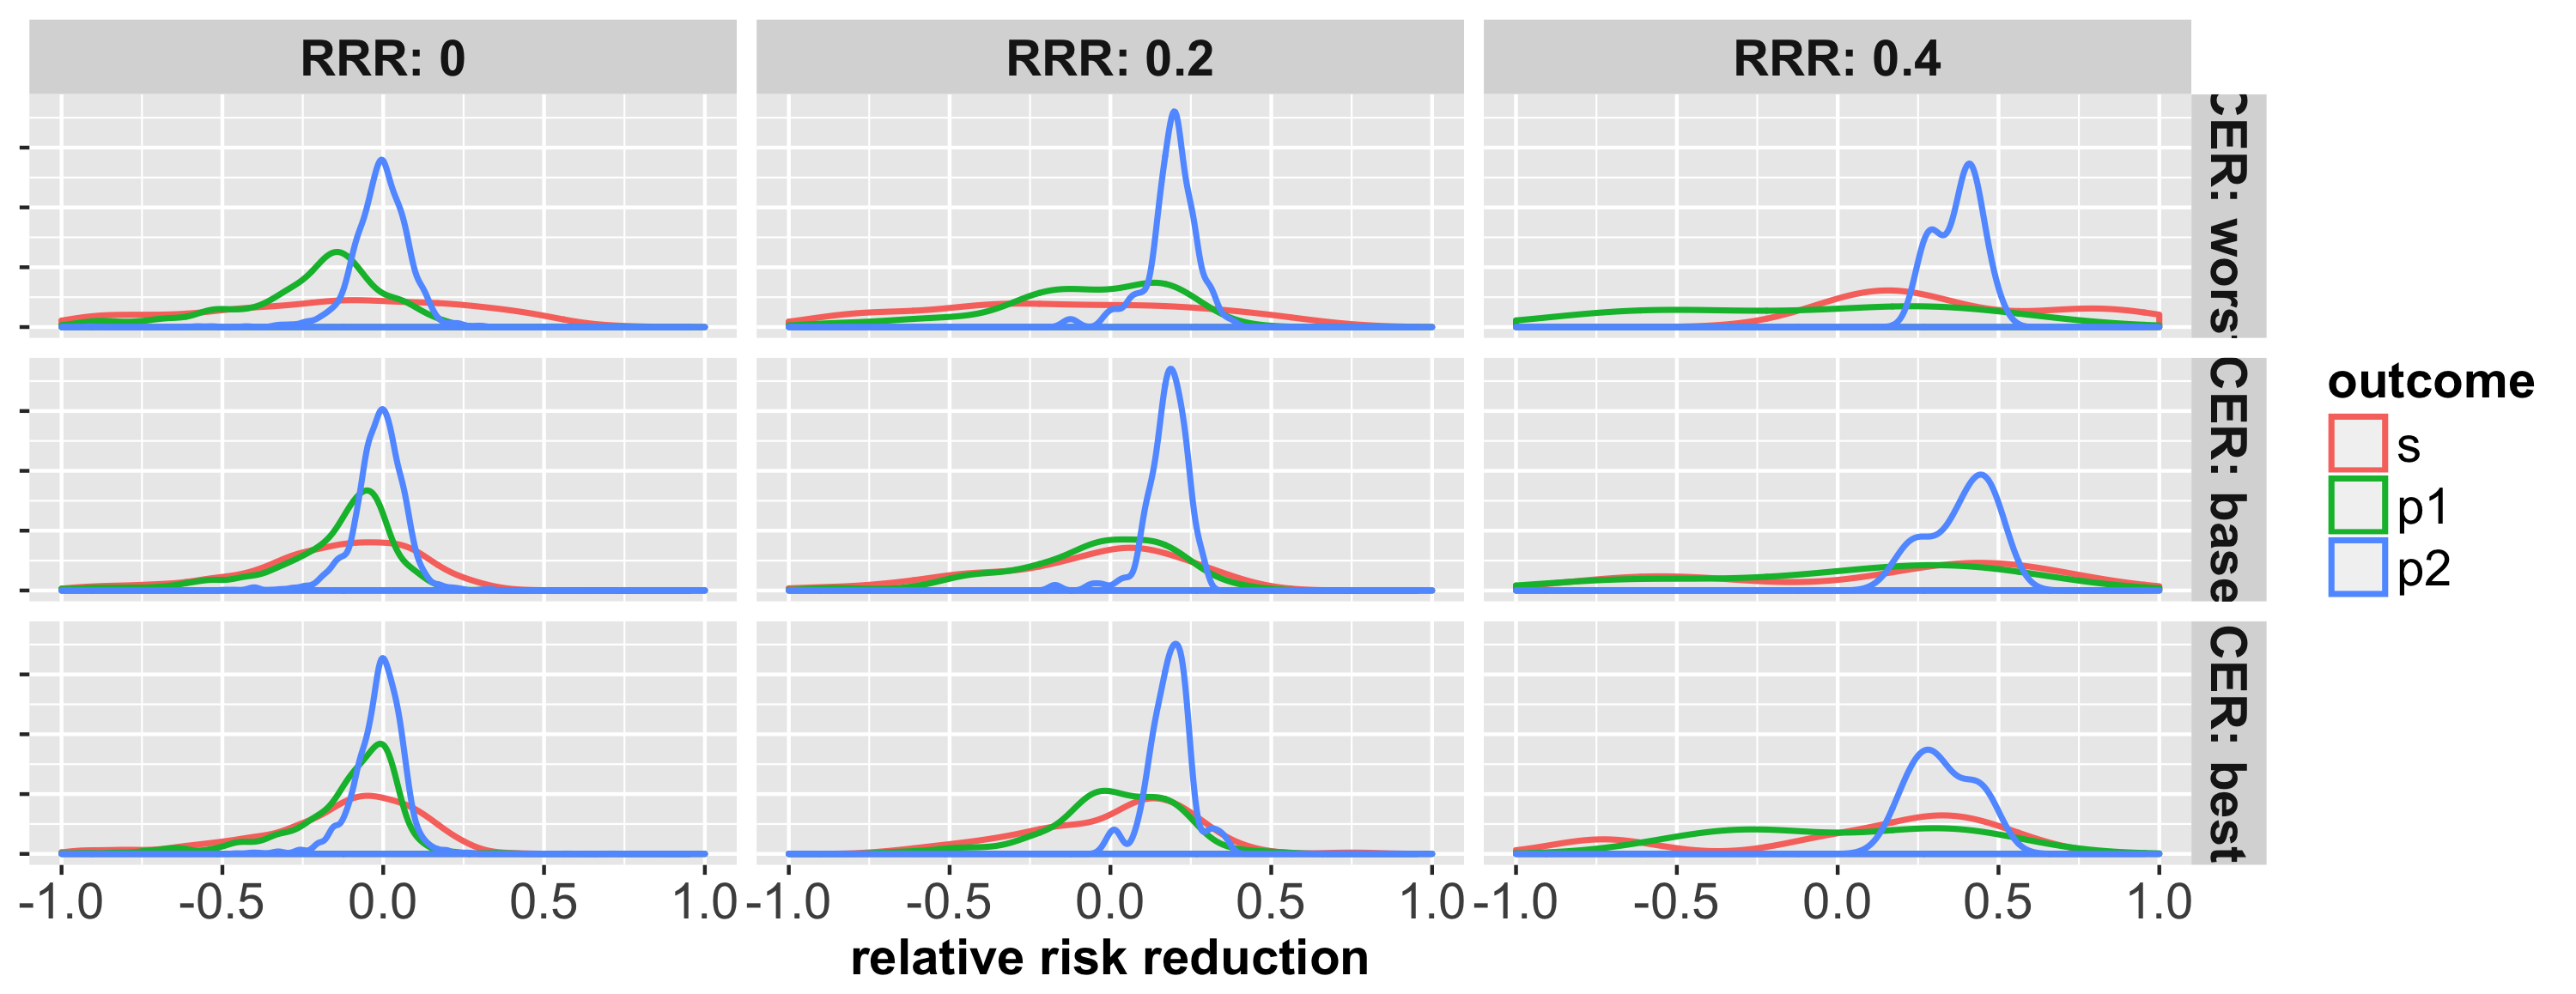
\includegraphics{../plots/3arm/RRRhat_futlp_3arm.png}
  \end{subfigure}
\end{figure}

\begin{figure}
\centering
  \caption{Distribution of relative risk reduction estimates after stopping early for superiority of (a) B.I. or (b)
  L.P. Results are presented for the control event rate (rows, BEST CASE ONLY for B.I?), four relative risk reductions (by columns) and the three outcomes (legend).}
  \begin{subfigure}{0.8\textwidth}
    \centering
    \caption{}
    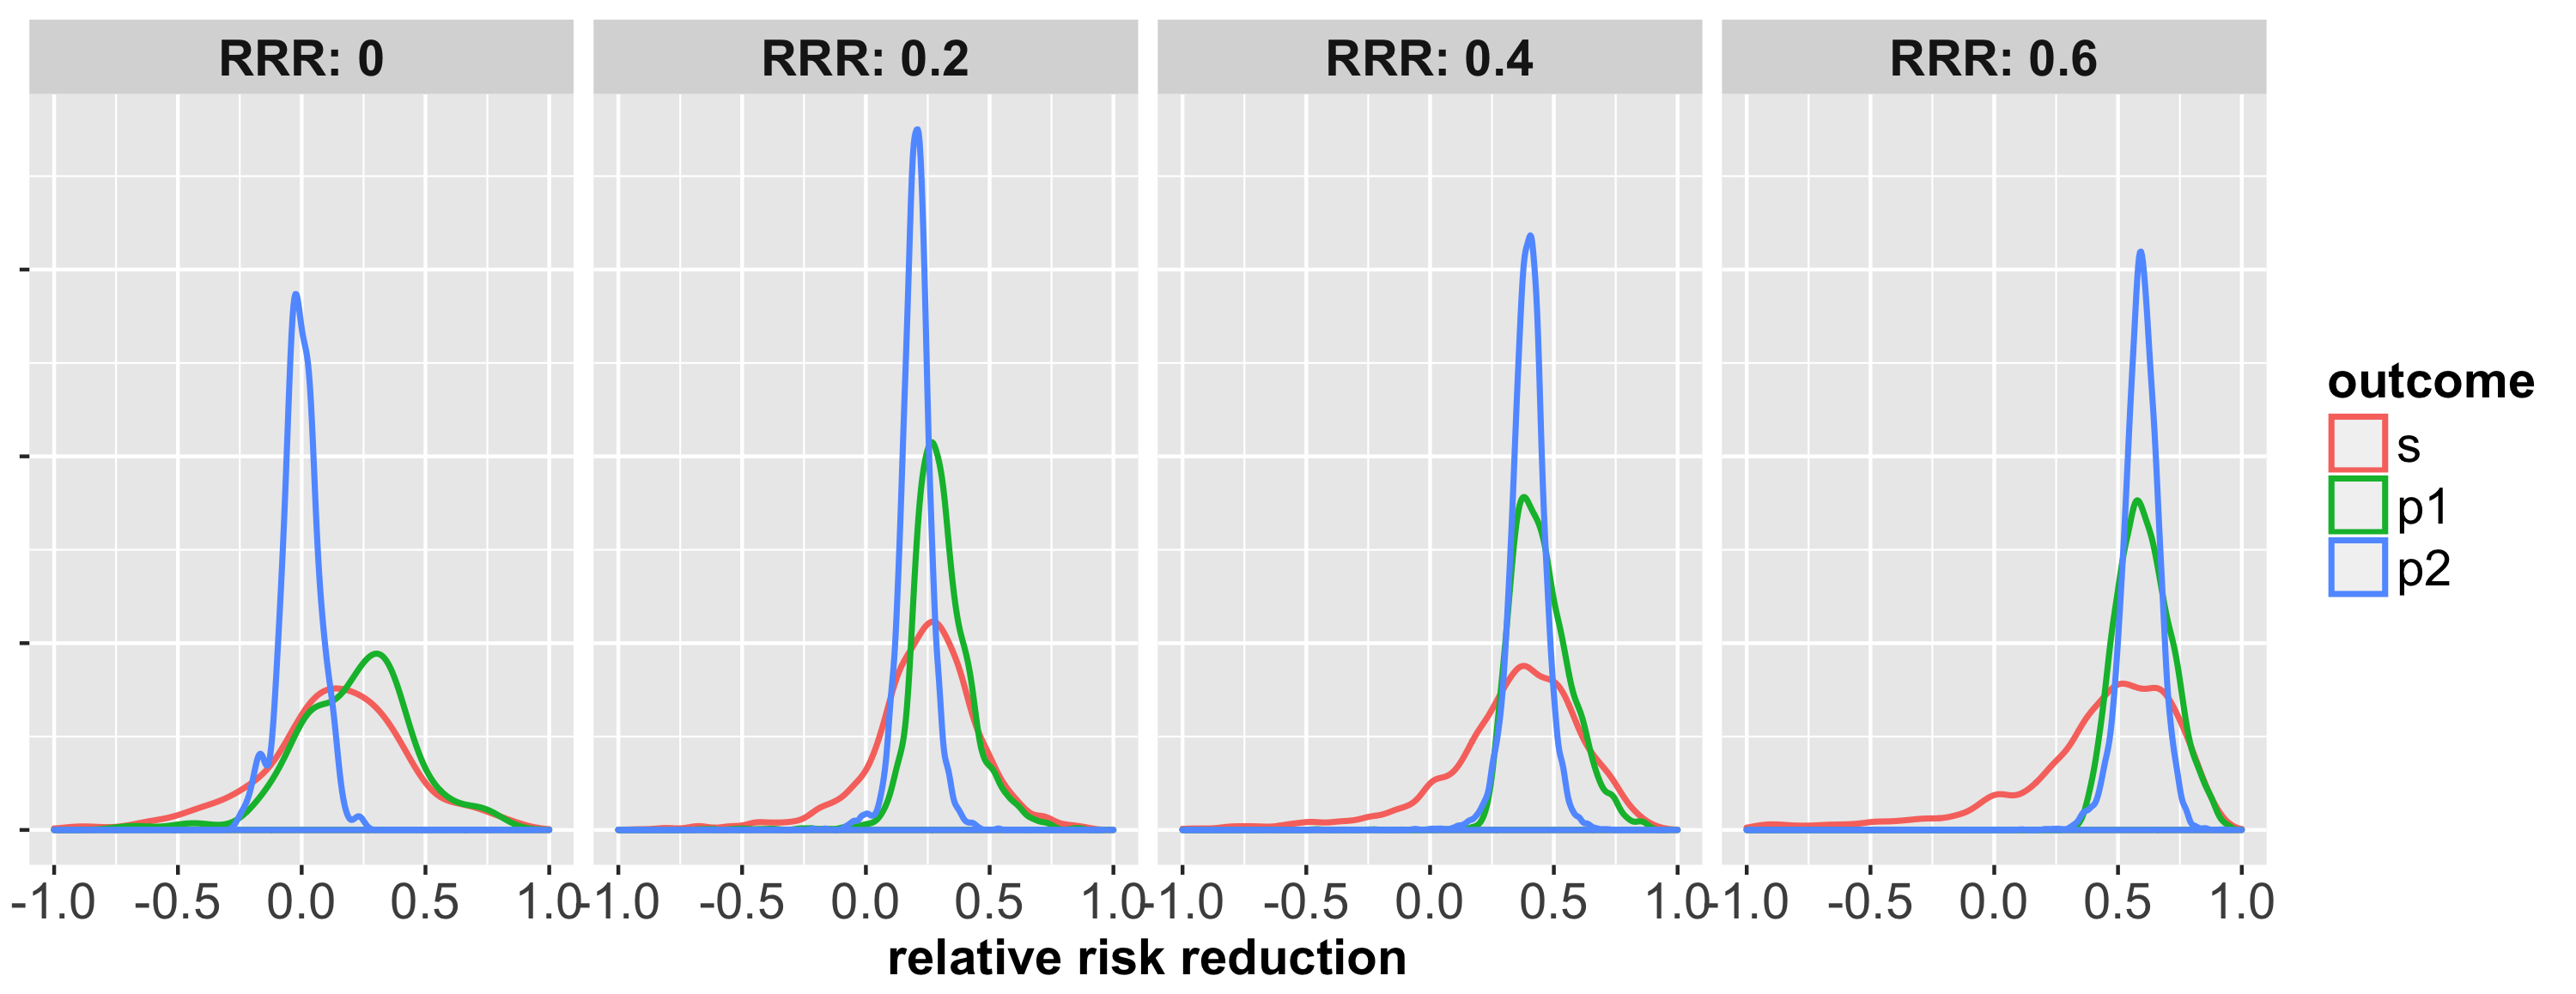
\includegraphics{../plots/3arm/RRRhat_supbi_3arm.png}
  \end{subfigure}
  \bigbreak
  \begin{subfigure}{0.8\textwidth}
    \centering
    \caption{}
    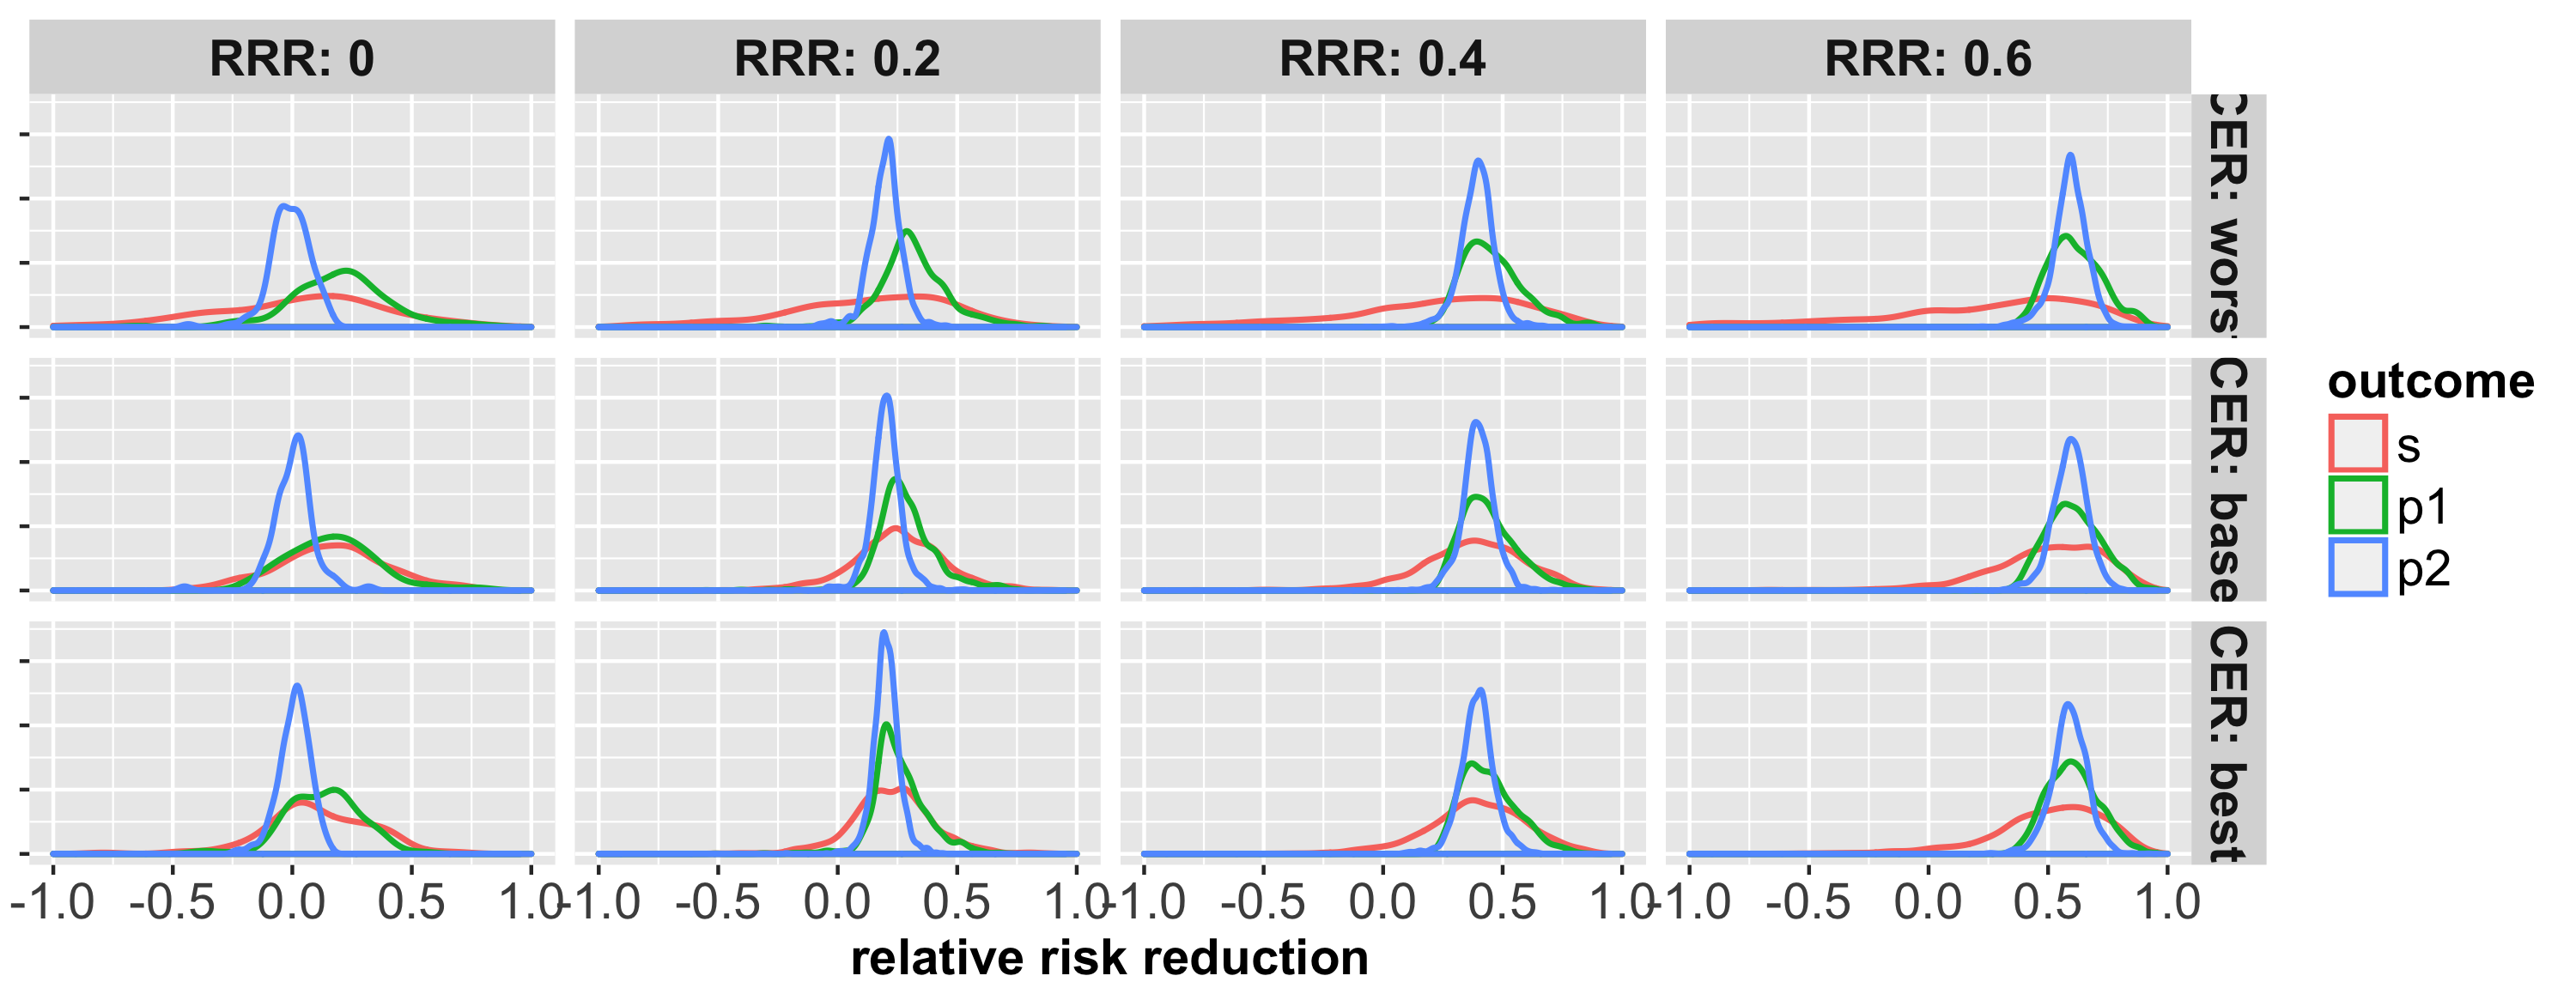
\includegraphics{../plots/3arm/RRRhat_suplp_3arm.png}
  \end{subfigure}
\end{figure}

\hypertarget{summary}{%
\subsubsection{Summary}\label{summary}}

For the two arm trial with stopping rules for the moderately permissive
outcome (p1), a superiority threshold of 0.99 should be employed to
ensure good control of Type 1 error (false positive rate less than 5\%).
Under this design, there is good power to detect outcomes p1 and p2
across most scenarios and a high proportion of p-values expected to be
less than 5\%. Additionally, there is little bias and good precision in
the RRR estimates of outcomes p1 and p2.

The multi-arm trial comparing B.I., L.P. and Control had higher expected
sample size at trial termination and a high proportion of significant
p-values is expected for RRR=20\%, 40\%, and 60\% for outcomes p1 and
p2. There is good precision in the RRR estimates of outcomes p1 and p2
when stopping for superiority, though this degrades when stopping for
futility.

\end{document}
